\part{Apéndices}



%%%%%%%%%%%%%%%%%%%%%%%%%%%%%%%%%%%%%%%%%%%%%%%%%%%%%%
\chapter{El mejor teorema: el teorema de \emph{Noether}}

	
\begin{tikzpicture}
	\fill [left color=red!50, right color=teal!50] (0,0) rectangle (6.5,.1);
	\fill [left color=teal!50, right color=blue!50] (6.5,0) rectangle (11.5,.1);
	\end{tikzpicture}



Reproduzco el artículo de 	\textbf{\textcolor{blue}{zientzia.eus}}



\textbf{El mejor teorema de Noether}. 2019/12/01. Urizar Lanz, Iñigo - Fisikan doktorea Iturria: Elhuyar aldizkaria

\textcolor{blue}{https://zientzia.eus/artikuluak/noetherren-teoremarik-politena/es/}



	\begin{figure}[H]
	\centering
	\includegraphics[width=.4\textwidth]{imagenes/apendices-01-01.png}
\end{figure}





\newpage
\includepdf[pages=-]{imagenes/MejorTeoremaNoether-ZientziaEus.pdf}



%%%%%%%%%%%%%%%%%%%%%%%%%%%%%%%%%%%%%%%%%%%%%%%%%%%%%%

\chapter{\emph{Emmy Noether}: alma, corazón y vida}

\section [\emph{Emmy Noether}, la matemática judía que se sobrepuso al machismo académico y al nazismo]{\emph{Emmy Noether}, la matemática judía que se sobrepuso al machismo académico y al nazismo\sectionmark{\emph{Emmy Noether}: biografía}}
\sectionmark{\emph{Emmy Noether}: biografía}

\begin{small} 
En una época en la que las mujeres no podían acceder a la universidad, ella acabó superando a sus coetáneos y siendo reverenciada por grandes figuras como Einstein o David Hilbert 
\footnote{\emph{``Emmy Noether, la matemática judía que se sobrepuso al machismo académico y al nazismo''.} Por E. Zamorano, 02/09/2021, artículo publicado en ``El confidencial''}


A Noether se le pusieron muchas cosas en contra cuando decidió dedicarse a la vocación de su vida: el álgebra y la física teórica. En primer lugar, el hecho de ser mujer en una época en la que estaba prohibido su acceso a la universidad y, segundo, provenir de una familia judía ubicada en la ciudad bávara de Erlangen, por lo que tuvo que dejar atrás su Alemania natal para partir a Estados Unidos.


Cuando Noether ya descubrió su verdadera vocación, las mujeres estaban apartadas de la academia. No fue hasta 1903, año en el que la joven ya alcanzaba los 21 años de edad, cuando la Universidad de Erlangen comenzó a permitir que las mujeres se matricularan en sus distintas carreras. Entonces, decidió hacer un doctorado que no le serviría para dar clase, pues aunque podían estudiar, todavía no se les permitía llegar a la docencia. Ello no le desanimó ni le hizo desistir de su empeño de enseñar, pues comenzó a dar clases extraoficiales a los alumnos del doctorado sin poder cobrar. 

\textbf{Una universidad nada femenina} 

``Creo que el cerebro femenino no es adecuado para la producción matemática''. Esta fue la frase del entonces decano de la Universidad de Gotinga cuando Noether solicitó una plaza de profesorado en 1915, sin embargo, se mostró favorable a acogerle en el claustro como si fuera una excepción. Desafortunadamente, el Ministerio de Educación de Prusia no le concedió el permiso para tener plaza en la facultad y, de nuevo, Noether se las apañó para seguir en la vida académica por sus propios medios, enseñando bajo un seudónimo masculino. 

Cuatro años después, y tras muchos infructuosos esfuerzos por intentar dedicarse profesionalmente a la investigación matemática, la joven entusiasta seguía sin plaza en la universidad, pero lo que sí que había conseguido era haberse hecho un nombre entre sus coetáneos, como David Hilbert y Felix Klein, quienes intentaron por todos los medios conseguirle un puesto como Privatdozent, los tutores privados de aquellos alumnos a los que ningún profesor quería dar clase. 

El gran talento de Noether y su incipiente fama dentro de los cenáculos matemáticos (siempre masculinos) le encumbraron a postularse como profesora y miembro del Consejo de la Universidad de Gotinga. "Caballeros, el Consejo no es una casa de baños, así es que no veo por qué una mujer no puede formar parte de él", adujo Hilbert cuando comenzó a sonar su nombre como próxima admisión en dicho órgano universitario. No fue hasta 1919 cuando finalmente consiguió su derecho a enseñar en las aulas, pero el éxito y lo bueno estaba aún por llegar. 
 
Aunque por fin parecía estar establecida en Gotinga, la vida de Noether estaba a punto de volver a cambiar. Con la llegada de Hitler al poder se aprobó una ley que prohibía a los judíos impartir clase en las universidades alemanas, por lo que tuvo que huir a Estados Unidos. Así es como Gotinga recibió un telegrama en el que se solicitaba que seis profesores debían abandonar la docencia de forma inmediata. Esto no fue un problema para la académica. A pesar de que toda su vida había luchado por conseguir un puesto en la universidad y de la noche a la mañana se quedó sin él, estaba acostumbrada a bregar entre la incertidumbre y el desprecio de sus iguales. Antes por ser mujer, y para entonces por ser judía. 


Entonces, partió rumbo a Estados Unidos gracias a una cátedra ofrecida por la universidad para mujeres Bryn Marw, localizada en Pensilvania, donde también impartían clase más académicos alemanes exiliados. Así, fue mentora de cuatro mujeres más jóvenes que aspiraban a ser un día como ella y dedicarse al estudio de las matemáticas. En aquel momento, Albert Einstein enseñaba en el Instituto de Estudios Avanzados de Pricenton junto a otros intelectuales como Abraham Flexner o Oswald Weblen, quienes le invitaron a dar clases allí en 1934. 

\textbf{Una muerte repentina}

Desgraciadamente, su trayectoria académica se truncó cuando en abril de 1935 los médicos le detectaron un tumor pélvico muy avanzado que debía ser extirpado cuanto antes. Apenas cuatro días después de la intervención quirúrgica, murió de forma inesperada a raíz de una fiebre muy alta que le entró.  


En su funeral, el también matemático Hermann Weyl dedicó unas emocionadas palabras de despedida a su admirada profesora y compañera, que sin duda sirven de colofón perfecto para este breve repaso a su vida y legado: "En su corta vida, Noether revolucionó las matemáticas. Siguió enseñando y aprendiendo incluso cuando ni las mujeres ni los judíos eran bienvenidos en las universidades. Nos dejaste en tu mejor momento creativo como el eco de un trueno. Adiós, Emmy Noether, gran matemática y gran mujer. Aunque tus restos mortales se descompongan, siempre apreciaremos el legado que nos dejaste". 



``Si se hubiera de juzgar la labor de los matemáticos vivos más competentes, la señorita Noether ha sido de lejos el genio matemático más significativo producido desde que comenzó la educación superior de las mujeres''. Con esta frase, el mismísimo Albert Einstein repasaba la vida y el legado de la que es una de las mayores revolucionarias en el mundo de las matemáticas, cuyos hallazgos se siguen estudiando hoy en día. Emny Noether, nacida en 1882 en el estado alemán de Baviera, es sin duda uno de los iconos feministas más relevantes de la historia y de la ciencia, pues luchó incansablemente para hacerse un hueco en el siempre masculino mundo de las matemáticas, siendo además adulada y reconocida por su labor a posteriori por nombres tan importantes como David Hilbert (padre del formalismo) o por el algebrista holandés B. L. van der Waerden, quien dijo también de ella que su originalidad matemática ``estaba absolutamente más allá de cualquier comparación''.

\end{small}



%%%%%%%%%%%%%%%%%%%%%%%%%%%%%%%%%%%%%%%%%%%%%%%%%%%%%%%%
\chapter{Elementos de cálculo en varias variables: jacobianos y hesisanos.}
\chaptermark{Jacobianos y Hesianos}
\label{ap-CVV}

\textcolor{gris}{\emph{Aunque este apéndice no es necesario, se supone que el curso está dedicado a personas con conocimientos previos de física (haber cursados 2 o 3 años del grado de física), lo incluyo para aprovecharlo en posibles futuras versiones de otros cursos.}}

Los conceptos que veremos en este apéndice de jacobianos (generalización de la primera derivada) y hesianos (generalización de la derivada segunda) son importantes para el cálculo de extremos de funciones multivariadas.



\section{Derivada parcial}

\begin{itemize}
\item La derivada parcial de una expresión respecto de una variable se hace como la derivada tradicional pero considerando a las otras variables como constantes.
\item La derivada parcial de un vector es el vector formado por las derivadas parciales.	
\end{itemize}

\begin{example}
. $f:\, \mathbb R^3 \ \to \ \mathbb R^2 \ / \ (x,y,z) \ \rightsquigarrow  (f_1,f_2)=(x^2yz^3\, , \, e^x \sin y \ln z)$

\vspace{3mm} Calcular: $\quad \displaystyle \pdv{f}{x}	\, ; \quad 	\pdv{f}{y}	\, ; \quad \pdv{f}{z}$
\end{example}

$\displaystyle  \pdv{f}{x}=\left( \pdv{f_1}{x}\, , \, \pdv{f_2}{x} \right) = (2xyz^3\, , \, e^x\sin y \ln z )\, ;$
$\qquad  \displaystyle \pdv{f}{y}=\left( x^2z^3 \, , \, e^x\cos y \ln z \right)\, ;$
$\quad  \displaystyle \pdv{f}{z}=\left( 3x^2yz^2 \, , \, \dfrac{e^x \sin y}{z} \right)$

En un punto determinado, solo hay que sustituir. Por ejemplo,  $\quad \displaystyle \eval{\pdv{f}{z}}_{(0,\pi/2,1)}=(0,1)$


\section{Jacobiano}

Es la generalización del concepto de derivada para funciones de varas variables. Se escribe como la matriz de las derivadas parciales de la función y se le llama así en honor a \emph{Carl Gustav Jacobi}y se representa por la letra $\boldsymbol J$.

$f: \, \mathbb R^n \, \to \, \mathbb R^m \, / \ \ f(x_1,x_2,\cdots, x_n)\, = \, (f_1, f_2, \cdots , f_m)$

\begin{equation}
\label{ap.jacobiano}
\subrayado{ \  \boldsymbol{ 
J \ = \ \mqty(
 \displaystyle \pdv{f_1}{x_1} & \displaystyle \pdv{f_1}{x_2} & \cdots & \displaystyle \pdv{f_1}{x_n} \\ \\
 \vdots & \vdots & \ddots & \vdots \\ \\
 \displaystyle \pdv{f_m}{x_1} & \displaystyle \pdv{f_m}{x_2} & \cdots & \displaystyle \pdv{f_m}{x_n} 
 )_{m\times n}
\ } }	
\end{equation}

\begin{example}
.	$f:\mathbb R^2 \to \mathbb R^2 \; / \, f(x,y)=(x^2+y^2,x-y)\, , \ $	 calcula $\, J_f$
\end{example}


$f_1=x^2+y^2;\quad f_2=x-y \quad \to \qquad J_f=\mqty( \displaystyle \pdv{f_1}{x} &  \displaystyle \pdv{f_1}{y} \\  \displaystyle \pdv{f_2}{x} &  \displaystyle \pdv{f_2}{y} )= \mqty( 2x & 1 \\ 2y & -1 )$

\section{Derivadas parciales de segundo orden}

Se definen las derivadas segundas como $\quad \displaystyle \pdv[2]{f_i}{x_j}=\pdv{x_j} \left( \pdv{f_i}{x_j} \right) \ $  

y las derivadas cruzadas como $\quad  \displaystyle \pdv[2]{f_i}{x_j}{x_k}=\pdv{x_j} \left( \pdv{f_i}{x_k} \right)$

\textbf{Teorema de Schwartz}. Si $f$ es de clase $\mathcal C^2$, continua con derivadas continuas hasta, al menos, segundo grado $\ \Rightarrow \ $ las \emph{derivadas cruzadas} conmutan: $\quad  \displaystyle \pdv[2]{f_i}{x_j}{x_k}= \pdv[2]{f_i}{x_k}{x_j}$

\begin{example}
.	$f(x,y,z)=(xy^2,yz^2)\ $	calcula todas las derivadas de orden 2.
\end{example}

$\displaystyle \pdv[2]{f}{x}=\pdv{x}\left(\pdv{f}{x}\right)=\pdv{x}(y^2,0)=(0,0);\quad \pdv[2]{f}{y}=\pdv{y}(2xy,z^2)=(2x,0); \quad \pdv[2]{f}{z}=\pdv{z}(0,2zy)=(0,2y)$

$\displaystyle \pdv[2]{f}{x}{y}=\pdv{x} \left( \pdv{f}{y} \right) = \pdv{x} (2xy,z^2)=(2y,0) \quad  \mqty{ = \\ \text{\tiny{Th.Schwartz}} } \quad \pdv[2]{f}{y}{x}=\pdv{y} \left( \pdv{f}{x} \right) = \pdv{y} (y^2,0)=(2y,0)$

$\displaystyle \pdv[2]{f}{x}{z}=\pdv{x}(0,2zy)=(0,0)=\pdv[2]{f}{z}{x}\, ;  \qquad  \qquad \qquad \pdv[2]{f}{z}{y}= \pdv[2]{f}{y}{z}=\pdv{y}(0,2yz)=(0,2z)$

\section{Derivada total y diferencial}

$f:\mathbb R^n \to \mathbb R^m \ / \ x_i=x_i(t)\, , \ \forall i=1,\cdots, n \quad \to \quad f=f(t)$


\begin{equation}
\label{app.derivada-total}
\boldsymbol{
\displaystyle \dv{f}{t} \ = \ 	\pdv{f}{x_1} \dv{x_1}{t} \ + \ \pdv{f}{x_2} \dv{x_2}{t} \ + \ \cdots \ + \ \pdv{f}{x_n} \dv{x_n}{t} \ = \ \sum_{i=1}^n \, \pdv{f}{x_i} \dv{x_i}{t}    
}
\end{equation}


\begin{equation}
\label{app.diferencial}
\boldsymbol{ \dd f \ = \ \pdv{f}{x_1} \dd x_1 \ + \ \pdv{f}{x_2} \dd x_2 \ + \ \cdots \ + \ \pdv{f}{x_n} \dd x_n \ = \ \sum_{i=1}^n \, \pdv{f}{x_i} \dd x_i
\displaystyle  
}
\end{equation}

\begin{example}
.	$f: \mathbb R^2 \to \mathbb R \ / \ f(x,y)=x^2-y^2 \qquad  \text{donde } \quad x=t\cos t \, ; \ \ y=\cos t + \sin t $ 	

\vspace{3mm} Calcula $\quad \displaystyle \dv{f}{t} \ \text{ y } \ \dd f$
\end{example}


$\displaystyle \dv{f}{t}= 2x \dv{x}{t} - 2y \dv{y}{t} = 2(t\cos t) [\cos t - t\sin t] -2(\cos t + \sin t) [-\sin t + \cos t]$

Previamente, de las expresiones de $x$ e $y$ calculamos: $\quad \dd x=(\cos t - t \sin t )\, \dd t \ $ y $\ \displaystyle \dd y=(-\sin t+\cos t)º, \dd t$

$\displaystyle \dd f = 2x \, \dd x -2y \, \dd y =\ \textcolor{gris}{ 2(t\cos t) [\cos t - t\sin t] \, \dd t  -2(\cos t + \sin t) [-\sin t + \cos t]\, \dd t }$


\section{Derivada direccional y gradiente}

$f:\mathbb R^n \to \mathbb R^m\, ; \ \ \hat v \ \text{vector unitario. } \  $ Se llama \emph{derivada direccional} de $f$ en la dirección $\hat v$ a $\quad \boldsymbol{J_f\, \hat v}$

\textcolor{gris}{Dimensionalmente es una matriz $m \times 1$, ya que $\ (J_f)_{m \times n} \,  ( \hat v )_{n \times 1}$ }


El \emph{gradiente} es un caso particular del jacobiano para funciones $f:\mathbb R^n \to \mathbb R$, \emph{funciones escalares}, se representa como $\nabla f$

\begin{equation}
\label{app.gradiente}
\boldsymbol{
\nabla f \ = \ \left( \, \pdv{f}{x_1}\, , \  \pdv{f}{x_2}\, , \ \cdots \, , \  \pdv{f}{x_n} \, \right) \, 
}	\in \mathbb R^n \ (\text{vector } \mathbb R^n )
\end{equation}


\begin{example}
.	$f(x,y)=x^2-xy+y^2 \, . \ \  $ Calcular el gradiente de $f$	
\end{example}

$\displaystyle \nabla f = \left( \pdv{f}{x}, \pdv{f}{y} \right) = (2x-y,-x+2y)$


\section{Hesiano}

Para una función escalar, se llama \emph{hesiano} al \emph{jacobiano del gradiente}. Es la matriz de las derivadas segundas.


$f:\mathbb R^n \to \mathbb R \quad \to \quad \nabla f: \mathbb R^n \to \mathbb R^n \quad \Rightarrow \quad \boldsymbol{ H_f \ = \ J_{\nabla f} }$

\begin{equation}
\label{app.hesiano}
\boldsymbol{ \subrayado{ \ 
H_f \ = \ \mqty(
\displaystyle \pdv[2]{f}{x_1} & \displaystyle \pdv[2]{f}{x_1}{x_2} & \displaystyle \pdv[2]{f}{x_1}{x_3} & \cdots & \displaystyle \pdv[2]{f}{x_1}{x_n} \\ \\
\displaystyle \pdv[2]{f}{x_2}{x_1} &  \displaystyle \pdv[2]{f}{x_2} & \displaystyle \pdv[2]{f}{x_2}{x_3} & \cdots  & \displaystyle \pdv[2]{f}{x_2}{x_n} \\ \\
\vdots & \vdots & \vdots & \ddots & \vdots \\ \\
\displaystyle \pdv[2]{f}{x_n}{x_1} &  \displaystyle \pdv[2]{f}{x_n}{x_2} & \displaystyle \pdv[2]{f}{x_n}{x_3} & \cdots & \displaystyle \pdv[2]{f}{x_n}
)	
\ } }
\end{equation}


\begin{example}
.	$f(x,y)=x^2-x^2y+y^3	 \, , \ \ \text{ calcula } \ H_f$
\end{example}

Claramente (polinómica) $f$ es de clase $\mathcal C^2$ y se cumple el teorema de Schwartz, las derivadas cruzadas conmutan.

$ \displaystyle \pdv{f}{x}=2x-2xy \qquad \qquad \pdv{f}{y}=-x^2+3y^2$

$\begin{cases}
\ \ \displaystyle \pdv[2]{f}{x}=\pdv{x}(2x-2xy)=2-2y \\ \\
\ \ \displaystyle \pdv[2]{f}{y}=\pdv{y}(-x^2+3y^2)=6y \\ \\
\ \ \displaystyle \pdv[2]{f}{x}{y}=\pdv[2]{f}{y}{x}=\pdv{y}(2x-2xy)=-2x 
\end{cases} \qquad \rightarrow \qquad H_h=\mqty(2-2y&-2x\\-2x&6y)$


\section{Derivada de la función compuesta}

$f:\mathbb R^n \to \mathbb R^m\, , \quad g:\mathbb R^m \to \mathbb R^p \quad \Rightarrow \qquad g \circ f :\mathbb R^n \to \mathbb R^p \ / \ (g\circ f)(x)=g(f(x))$

\begin{equation}
\label{app-deriv-cmpta}
\exists (J_f)_{m\times n}\, , \ \ \exists (J_g)_{p\times m} \quad \Rightarrow \quad \exists \, \  \boldsymbol{(J_{g\circ f})_{p\times n} \ = \ J_g(f(x))\cdot J_f(x)}
\end{equation}


\begin{example}
.	$f : \mathbb R^2 \to \mathbb R^3 \ \ / \ \ f(a,b)=(a^2-b\cos a\, , \ ab\, , \ a^3+b^3) \, ; \qquad 	g : \mathbb R^3 \to \mathbb R \ \ / \ \ f(x,y,z)=x-y^2+z$

\vspace{3mm} Calcular $\ \ J_{g\circ f}$
\end{example}

$g\circ f :\mathbb R^2 \to \mathbb R \ \ / \ \ (g\circ f)(a,b)=g(f(a,b)) \in \mathbb R$

$\triangleright \quad J_g(x,y,z)=\mqty( \displaystyle \pdv{g}{x} & \displaystyle \pdv{g}{y} & \displaystyle \pdv{g}{z})_{1\times 3}= \mqty(1&-2y&1) \quad \to \quad J_g(f(a,b))=\mqty(1& -2ab&1)$

$\triangleright \quad J_f= \mqty( \displaystyle \pdv{f_1}{a} & \displaystyle \pdv{f_1}{b} \\ \displaystyle \pdv{f_2}{a} & \displaystyle \pdv{f_2}{b} \\ \displaystyle \pdv{f_3}{a} & \displaystyle \pdv{f_3}{b})_{3\times 2}=\mqty(2ab\sin a & -\cos a \\ b&a\\3a^2&3b^2)$

$\triangleright \triangleright \quad J_{g\circ f} =\mqty(1& -2ab&1) \cdot \mqty(2ab\sin a & -\cos a \\ b&a\\3a^2&3b^2) = (2a+b\sin a-2ab^2+3a^2\, , \ -\cos a -2a^2b+3b^2)$

\rule{200pt}{0.1pt}

Si primero calculamos $J_{g\circ f}$ y luego su jacobiano hemos de obtener, obviamente,  el mismo resultado:


$(g\circ f)(a,b)=g(f(a,b))=g(a^2-b\cos a\, , \ ab\, , \, a^3+b^3) = (a^2-b\cos a)- (a^2b^2)+(a^3+b^3)= $

$=a^3+b^3+a^2-a^2b^2-b\cos a$


$J_{g\circ f}  = \mqty( \displaystyle \pdv{g\circ f}{a} \, , \,  \displaystyle \pdv{g\circ f}{b} )_{1\times 2} = (2a+b\sin a-2ab^2+3a^2\, , \ -\cos a -2a^2b+3b^2)$ \hspace{3cm} $\Box$



\section{Aplicaciones de la jacobiana (jacobiano)}

Se llama \textbf{\emph{jacobiano}} al determinante de la matriz jacobiana.

\begin{itemize}
\item $\textbf{Teorema de la función inversa:} \quad \textbf{si } \ \boldsymbol{ \det(J_f) \neq 0 \ \Rightarrow \ \exists \, f^{-1} } $
\item \textbf{Determinación de puntos críticos} . Hay que encontrar los puntos que hacen $\ \boldsymbol {J_f=0} \, , \  $  el que sean máximos, mínimos, puntos de silla lo determinará la matriz hesiana $\ H_f$
\item \textbf{Aproximación lineal de una función}: $\quad \boldsymbol{ f(x) \approx f(p) + J_f(p)(x-p) }$
\item \textbf{Cambio de variable en integrales múltiples} $\quad \boldsymbol{\displaystyle \int f(x) \, \dd x \ = \ \int f(g(y) \, |\det J_g|\, \dd y}$

Cuando se hace un cambio de variable en una integral múltiple, por ejemplo $x=g(y)$ hay que multiplicar por el valor absoluto del jacobiano del cambio, $|\det(J_g)|$
\item \textbf{Cambio de coordenadas}
	\begin{itemize}
	\item \textbf{Coordenadas cilíndricas} $\quad x,y,z \ \to \ r,\theta, z \quad \text{con } \ \ \begin{cases} \ x=r\cos \theta \\ \ y=r\sin \theta \\ \ z=z \end{cases}$
	
	$J= \mqty(
	\displaystyle \pdv{x}{r} & \displaystyle \pdv{x}{\theta} & \displaystyle \pdv{x}{z} \\ 
	\displaystyle \pdv{y}{r} & \displaystyle \pdv{y}{\theta} & \displaystyle \pdv{y}{z} \\ 
	\displaystyle \pdv{z}{r} & \displaystyle \pdv{z}{\theta} & \displaystyle \pdv{z}{z} \\ 
	)= \mqty( \cos \theta & -r\sin \theta & 0 \\ \sin \theta & r\cos \theta & 0 \\ 0 & 0 & 1 ) \qquad \to \quad \det(J)=r>0$ 
	
	\hspace{5cm} $\dd V \ = \  \dd x \, \dd y\, \dd z \ = \  \boldsymbol r  \, \dd r \, \dd \theta \, \dd z$
	\item \textbf{Coordenadas esféricas} $\quad x,y,z \ \to \ \rho,\theta, \phi \quad \text{con } \ \ \begin{cases} \ x=\rho \sin \phi \cos \theta \\ \ y=\rho \sin \phi \sin \theta \\ \ z=\rho \cos \phi \end{cases}$
	
	$J= \mqty(
	\displaystyle \pdv{x}{\rho} & \displaystyle \pdv{x}{\theta} & \displaystyle \pdv{x}{\phi} \\ 
	\displaystyle \pdv{y}{\rho} & \displaystyle \pdv{y}{\theta} & \displaystyle \pdv{y}{\phi} \\ 
	\displaystyle \pdv{z}{\rho} & \displaystyle \pdv{z}{\theta} & \displaystyle \pdv{z}{\phi} \\ 
	)= \mqty( 
	\sin \phi \cos \theta & \rho \cos \phi \cos \theta & -\rho \sin \phi \sin \theta \\
	\sin \phi \sin \theta & -\rho \cos \phi \sin \theta & \rho \sin \phi \cos \theta \\
	\cos \phi & -\rho \sin \phi & 0 
	 ) \qquad \to $
	 
	 $\to \quad \det(J)=\rho^2 \sin \phi \qquad |\det J|=|\sin \phi|$ 
	
	\hspace{5cm} $\dd V \ = \  \dd x \, \dd y\, \dd z \ = \  \boldsymbol{ \rho^2  \, |\sin \phi|} \,  r \, \dd r \, \dd \theta \, \dd \phi$
	\end{itemize}
\end{itemize}


\begin{figure}[H]
	\centering
	\includegraphics[width=.75\textwidth]{imagenes/apendices-01-11.png}
\end{figure}



%%%%%%%%%%%%%%%%%%%%%%%%%%%%%%%%%%%%%%%%%%%%%%%%%%%%%%%%%%%%%%%%
\chapter{Series de 	\emph{Fourrier}}
\label{ap-SF}

Utilizaremos la siguiente similitud con vectores:

$\vec v \in \mathbb R^n; \quad \{ e_1,e_2,\cdots , e_n \} \ $ una base de $\mathbb R^n \ \to \ \exists a_1,a_2,\cdots ,a_n \in \mathbb R \ / \ \vec v= a_1e_1+a_2e_2+ \cdots + a_ne_n$

Si $\ \{ e_1,e_2,\cdots , e_n \} \ $ es una bases ortonormal, existe una relación directa entre las componentes $ a_1,a_2,\cdots ,a_n$ del vector $\vec v$ y los vectores de la base a través del producto escalar:

Por ejemplo, $\ \ \vec v \cdot e_2 = a_1 \cancelto{0}{e_1 \cdot e_2} +a_2 \cancelto{1}{e_2 \cdot e_2}+ a_3 \cancelto{0}{e_3 \cdot e_2} \cdots + a_n \cancelto{0}{e_n \cdot e_1 }=a_2\, , \ $ luego

\vspace{-3mm}

$$\boldsymbol{ \vec v= a_1e_1+a_2e_2+ \cdots + a_ne_n=\displaystyle \sum_{i^1}^n a_i e_i \qquad \text{ con } \quad a_i=\vec v \cdot e_i }$$

 
\vspace{-3mm} Pensemos ahora en un espacio vectorial de dimensión infinita, el de las funciones reales de variable real bien comportadas, que denotaremos por la letra $\mathcal F$ \textcolor{gris}{(continuas, derivables, ...)}
Supongamos que $\ \{b_1,b_2, \cdots \} \ $ es una base de $\mathcal F$, entonces, cualquier función $f\in \mathcal F$ se podrá escribir de forma única como combinación lineal de los vectores de esa base : $\ f(x)=a_1b_1(x)+a_2b_2(x)+\cdots $

Si la base es \emph{ortogonal}, $\ b_i\cdot b_j = 0$, pero ?`qué es el producto escalar de funciones?


\begin{multicols}{2}

\underline{Discretización del problema}:

Supongamos que la variable $x$ solo toma valores en $x_1,x_2,\cdots x_5$, entonces, 

$b_1=(b_1(x_1),b_1(x_2),\cdots ) \text { y } b_2=(b_2(x_1),b_2(x_2),\cdots ) $ y definimos:

$b_1\cdot b_2=b_1=b_1(x_1)b_2(x_1) + b_1(x_2) b_2(x_2) +\cdots  = \sum_n b_1(x_n)b_2(x_n)\in \mathbb R$

En el caso continuo, para $f(x) \in [a,b]$ definimos

$b_1(x)\cdot b_2(x) =\displaystyle \int_a^b b_1(x)b_2(x) \, \dd x$
\begin{figure}[H]
	\centering
	\includegraphics[width=.45\textwidth]{imagenes/apendices-01-12.png}
\end{figure}	
\end{multicols}


\section{Serie de \emph{Fourrier}}

Fourrier demostró que $\ \{\cos x, \cos 2x, \cos 3x , \cdots , \sin x, \sin 2x, \sin 3x, \cdots , 1 \} \ $ es una base de $\mathcal F$, por ello, 

$$\boldsymbol{ f(x)} \ = \ a_0+a_1\cos x+a_2\cos 2x + \cdots +b_1\cos x + b_2 \sin 2x + \cdots \ = \  \displaystyle \boldsymbol{ \sum_{n=0} a_n \cos nx \ + \  \sum_{n=1} b_n \sin nx}$$

La descomposición de $f(x)$ en senos y cosenos de $nx$ solo es válida en $[-\pi,\pi]$.

Comprobemos que la base de Fourrier es \emph{ortogonal}:


$\cos n_1 x \cdot \cos n_1 x = \displaystyle \int_{-\pi}^{\pi} (\cos n_1x)^2\, \dd x = \int_{-\pi}^{\pi} \dfrac{1+\cos 2n_1x}{2}\, \dd x = \dfrac 1 2  \cancelto{2\pi}{\left[1\right]_{-\pi}^{\pi}} + \dfrac 1 2 \cancelto{0}{\left[ \dfrac {\sin 2n_1x}{2n_1} \right]_{-\pi}^\pi }=$

$=\dfrac 1 2 \, 2\pi = \pi$

$\displaystyle \cos n_1x \cdot \cos n_2 x = \int_{-\pi}^\pi \cos n_1 x \cos n_2 x \, \dd x = \dfrac 1 2 \int_{-\pi}^\pi [\cos(n_1+n_2)x+\cos(n_1-n_2)x] \, \dd x = $

$\displaystyle = \dfrac 1 2\cancelto{0}{\left[ \dfrac{\sin (n_1+n_2)x}{n_1+n_2} \right]_{-\pi}^\pi} +  \dfrac 1 2\cancelto{0}{\left[ \dfrac{\sin (n_1+n_2)x}{n_1-n_2} \right]_{-\pi}^\pi} =0 \quad (n_1 \neq n_2)$

Se puede comprobar que $ \quad \cos n_1\cdot \sin n_2 x = 0;\qquad \sin nx\cdot \sin n_x= 0;\qquad \sin n_1 x \cdot \sin n_2 x = \pi$

En conclusión: $\quad \boldsymbol{ \cos n_1\cdot \cos n_2 x = \pi \delta_{n_1,n_2};\quad \cos n_1 x \cdot \sin n_2 x = 0 ;\quad \cos n_1x \cdot sin n_2 x = \pi \delta_{n_1,n_2} }$

Donde $\quad \delta_{n_1,n_2}= \begin{cases} \ 0 & \text{si } \  n_1 \neq n_2 \\ \ 1 & \text{si } \ n_1=n_2 \end{cases}\, , \ $ es la \emph{delta de Kronecker}.

Lo que confirma que la base de Forurrier, $\ \{\cos x, \cos 2x, \cos 3x , \cdots , \sin x, \sin 2x, \sin 3x, \cdots , 1 \} \ $ es una base \textbf{ortogonal} $\qquad\Box$



\vspace{5mm} Para determinar los coeficientes $a_n$ y $b_n$ nos basamos en la propiedad vista al principio para vectores de $\mathbb R^n: \quad a_i=\vec v \cdot e_i\, , \ $ si la base es ortonormal y $\ a_i=\dfrac{\vec v \cdot e_i}{e_i \cdot e_i}\, , \ $ si la base. solo es ortogonal como es el caso de nuestra base de Fourrier para funciones.

En nuestro caso, $\quad a_k=\dfrac {f(x) \cdot \cos kx}{\cos kx \cdot \cos kx} =\dfrac {f(x) \cdot \cos kx}{\pi}\, ; \qquad b_k=\dfrac {f(x) \cdot \sin kx}{\sin kx \cdot \sin kx}=\dfrac {f(x) \cdot \sin kx}{\pi}$

Luego, 

$$ \boldsymbol{ a_n \ = \ \dfrac 1 \pi \, \int_{-\pi}^\pi f(x)\, \cos nx \, \dd x\, ; \qquad 	
b_n \ = \ \dfrac 1 \pi \, \int_{-\pi}^\pi f(x)\, \sin nx \, \dd x } $$


Recopilando:

\begin{large}
\begin{equation}
\subrayado{
\boxed{\quad 
\begin{split}
\label{app-series-fourrier} 
\\
\boldsymbol{ f(x) \ = \ \sum_{n=0} a_n \cos nx \ + \  \sum_{n=1} b_n \sin nx \qquad x\in [-\pi,\pi]} \\ \\
\boldsymbol{ a_n \ = \ \dfrac 1 \pi \, \int_{-\pi}^\pi f(x)\, \cos nx \, \dd x\, ; \qquad 	
b_n \ = \ \dfrac 1 \pi \, \int_{-\pi}^\pi f(x)\, \sin nx \, \dd x }
\\ \ 
\end{split}
\quad }
}
\end{equation}
\end{large}

\vspace{5mm}


\section{Serie compleja de \emph{Fourrier}}


$e^{i\boxplus}=1+\boxplus + \dfrac{\boxplus^2}{2!}+\dfrac{\boxplus^3}{3!}+ \cdots  \quad \to \quad \boldsymbol{ e^{ix}= }1+ix + \dfrac{(ix)^2}{2!}+\dfrac{(ix)^3}{3!}+ \cdots =1+ix-\dfrac{x^2}{2!}-i\dfrac{x^3}{3!}+\cdots=\left( 1-\dfrac {x^2}{2!}+\cdots \right) + \left( x-\dfrac {x^3}{3!}+\cdots \right)\, i\boldsymbol{ = \cos x + i\, \sin x } \quad \to \quad \boldsymbol{ e^{inx}= \underline{\cos nx} +i\, \underline{\sin nx}}$

Como el coseno es función par y el seno impar, $\boldsymbol{\ e^{-inx}=\cos nx - i\, \sin nx}$, con lo que sumando y restando las dos últimas expresiones tenemos: 

$$\boldsymbol{ \cos nx=\dfrac 1 2 \left( e^{inx} + e^{-inx} \right)\, ; \qquad \qquad  \sin nx=\dfrac 1 {2i} \left( e^{inx} - e^{-inx} \right) }$$

Llevando estos resultados a la serie de Fourrier, ec.\ref{app-series-fourrier}

$f(x)=\displaystyle \sum_{n=0}^\infty a_n \dfrac 1 {2} \left( e^{inx} + e^{-inx} \right) \ + \ \sum_{n=1}^\infty b_n \dfrac 1 {2i} \left( e^{inx} - e^{-inx} \right) = $

$\displaystyle = a_0\, + \,  
\sum_{n=1}^\infty \left[ \dfrac{a_n}{2} \left( e^{inx} + e^{-inx} \right) \ + \ \dfrac{b_n}{2i}  \left( e^{inx} - e^{-inx} \right) \right] =$

$\displaystyle = a_0 \, + \, \sum_{n=1}^\infty
 \left[ \left( \underbrace{\dfrac {a_n}{2}+\dfrac{b_n}{2i}}_{c_n} \right) e^{inx} \ + \  \left( \underbrace{\dfrac {a_n}{2}-\dfrac{b_n}{2i}}_{c_n^*} \right) e^{-inx}   \right]= a_0+\sum_{n=1}^\infty \left( c_n\, e^{inx} + c_n^*\, e^{-inx} \right) $


Al ser $\quad c_n=\dfrac {a_n}{2}+\dfrac{b_n}{2i}=\  \textcolor{gris}{\left[ \dfrac 1 i = -i \right]} \ = \dfrac{a_n}2-\dfrac{b_n}2\, i \to c_0=\dfrac 1 2 (a_0-\cancelto{0}{b_0}i )=\dfrac {a_0}2$

Como $\quad a_0=\dfrac {a_0}2+\dfrac {a_0}2=c_0+c_0=c_0+c_0^* \quad \textcolor{gris}{ (c_0\in \mathbb R)}\, , \ $ por otra parte, $a_0=c_0+c_0^*=c_0\cdot 1+c_0^*\cdot 1=c_0e^{i0x}+c_0^*e^{-i0x}$ y esto
nos permite incluir este término en el sumatorio y extenderlo desde que $\ n=0$.

$$\boldsymbol{ f(x)\ = \ \displaystyle \sum_{n=0}^\infty \left(\, c_n\, e^{inx} \ + \ c_n^*\, e^{-inx} \, \right)}$$

Los coeficientes son, $\quad \displaystyle \boldsymbol{ c_n=}\dfrac 1 2 (a_n-B_n\, i)= \dfrac 1 2 \left[ \dfrac 1 \pi \int_{-\pi}^pi f(x)\, \cos nx \, \dd x \ + \ \dfrac 1 \pi \int_{-\pi}^\pi f(x)\, \sin nx \, \dd x \right] = \dfrac 1 {2\pi} \int_{-\pi}^\pi f(x)\, (\cos nx -i\, \sin nx)\, \dd x  \boldsymbol{= \dfrac 1{2\pi} \int_{-\pi}^\pi f(x)\, e^{-inx}\, \dd x} \qquad n=0,1,2,\cdots$
  
$\boldsymbol{ \displaystyle c_n^*=\dfrac 1{2\pi} \int_{-\pi}^\pi f(x)\, e^{inx}\, \dd x = (c_n)^*}\, , \ $ calculado $c_n,\ c_n^*$ es su complejo conjugado.


Resumiendo:

\begin{equation}
	\label{app.trans.fourrier-compleja}
	\subrayado{ \ \boxed{ \ \ \boldsymbol{ f(x)\ = \ \displaystyle \sum_{n=0}^\infty \left(\, c_n\, e^{inx} \ + \ c_n^*\, e^{-inx} \, \right)} \qquad \qquad 
	\boldsymbol{ c_n\ = \ \displaystyle c_n^*=\dfrac 1{2\pi} \int_{-\pi}^\pi f(x)\, e^{inx}\, \dd x } \ \ } \ }
\end{equation}


\vspace{2mm}
\textbf{Propiedad de los coeficientes de la serie de Fourrier compleja}:

$\boldsymbol{c_n^*} \ = \ \displaystyle \dfrac 1{2\pi} \int_{-\pi}^\pi f(x)\, e^{-i(-n)x}\, \dd x \ = \ \boldsymbol{c_{-n}}\quad$ con esto, podemos escribir

$f(x)=\displaystyle \sum_{n=0}^\infty \left(\, c_n\, e^{inx} \ + \ c_{-n}\, e^{-i(-n)x} \, \right) = \sum_{n=0}^\infty c_n\, e^{inx} \ + \ \sum_{n=0}^\infty c_{-n} \, e^{i(-n)x} = \ \textcolor{gris}{[\,-n \to m \, ]} \ = $

$\displaystyle =
\sum_{n=0}^\infty c_n\, e^{inx} \ + \ \sum_{m=-\infty}^0 c_{m} \, e^{imx} = \ \textcolor{gris}{ [\, m \to n \, ]} \ = \sum_{n=-\infty}^\infty c_n\, e^{inx}\, , \ $ que es la forma compacta de escribir la serie de Fourrier compleja.

\vspace{5mm}
\begin{myblock}{Serie de Fourrier compleja. Forma compacta.}
\begin{equation}
\label{app-TFC}
\boldsymbol{ \subrayado{\ \boxed { \ \ 
f(x)\ = \ \sum_{n=-\infty}^\infty c_n\, e^{inx} \, ; \qquad c_n\ = \ \displaystyle c_n^*=\dfrac 1{2\pi} \int_{-\pi}^\pi f(x)\, e^{inx}\, \dd x
\ \ } \  } }	
\end{equation}	

Con $\quad \bold{ c_{-n} \ = \ c_n^* } \ $  y con $\quad \boldsymbol{ f(x) \in [-\pi,\pi] }$ 
\end{myblock}

\vspace{5mm} Establecemos un cambio de variable de modo que $ \ x\in [-\pi,\pi] \ $ se transforme en $\ y\in [-L/2,L/2]\ \to \ y=Ax\,:\ y=L/2 \leftrightarrow x=\pi \ \to \ A=\/2\pi$ El cambi a efectuar es $\ \boldsymbol y=\dfrac L{2\pi} x \ \to \ \dd y= \dfrac L{2\pi} \dd x \ \to \ \dd x = \dfrac{2\pi}L \dd y:$


$c_n=\displaystyle \dfrac 1 {2\pi} \int_{-L/2}^{L/2} f(y)\, e^{-i n \frac{2\pi}{L}y}\, \dfrac{2\pi}L \, \dd y= \dfrac 1 L \int_{-L/2}^{L/2} f(y)\, e^{-i\frac{2\pi n}{L} y}\, \dd y \quad $
y $\quad \displaystyle f(y)=\sum_{-\infty}^{+\infty} c_n\, e^{i\frac{2\pi n}{L} y}$

Como la variable $y$ es muda, podemos escribir:

\vspace{5mm}
\begin{myalertblock}{Serie de Fourrier compleja. Forma compacta.}
\begin{equation}
\label{TFC2}
\boldsymbol{ \subrayado{\ \boxed { \ \ 
f(x)\ = \ \sum_{-\infty}^{+\infty} c_n\, e^{i\dfrac{2\pi n}{L} x} \, ; \qquad c_n\ = \ \displaystyle c_n^*=\dfrac 1 L \int_{-L/2}^{L/2} f(y)\, e^{-i\dfrac{2\pi n}{L} x}\, \dd x \ \ } \  } }	
\end{equation}	

Con $\quad \bold{ c_{-n} \ = \ c_n^* } \ $  y con $\quad \boldsymbol{ f(x) \in [-L/2,L/2] }$ 
\end{myalertblock}

\section{Serie de \emph{Fourrier} dependiente del tiempo}

La versión continua de la serie de Fourrier que acabamos de ver, llamando $\ \boldsymbol{k_n=\dfrac{2\pi n}L }\ $ es $\quad \displaystyle f(x)=
\sum_{-\infty}^{+\infty} c_n\, e^{i\,k_n \, x} \, , \ $ con $\ c_n^*=c_{-n}$

Para tener una $f(x,t)$, dependiente también del tiempo, solo podemos incluir esa dependencia en los coeficientes $c_n(t)$, con lo que $\quad \displaystyle f(x,t)=\sum_{-\infty}^{+\infty} c_n(t) \, e^{i\,k_n \, x}$

Si lo que deseamos es que $f(x,t)$ represente a una onda, se deberá cumplir la ecuación general de ondas: $\ \quad \displaystyle \pdv[2]{f}{t}-v^2\pdv[2]{f}{x}=0$, siendo $v$ la velocidad de propagación de la onda. Esto determinará quienes son los coeficientes $c_n(t)$. 

Cálculos: $\quad \displaystyle \pdv[2]{f}{t}=\sum_{-\infty}^{+\infty} \ddot c_n(t) \, e^{i\,k_n \, x}\, ; \qquad \pdv[2]{f}{x}=\sum_{-\infty}^{+\infty} c_n(t) \, (ik_n)^2\, e^{i\,k_n \, x}=-\sum_{-\infty}^{+\infty} c_n(t) \,k_n^2\;  e^{i\,k_n \, x}$

Sustituyendo en la ecuación de ondas, 

$\displaystyle \sum_{-\infty}^{+\infty} \ddot c_n(t) \, e^{i\,k_n \, x} +v^2\, \sum_{-\infty}^{+\infty} c_n(t) \,k_n^2\;  e^{i\,k_n \, x} = \sum_{-\infty}^{+\infty} (\ddot c_n+v^2k_n \, c_n) e^{ik_n x}=0 \quad \Rightarrow \quad \ddot c_n(t)+v^2k_n \, c_n(t)=0$

Llamando $\omega_n=v|k_n| \ \to \ \omega_n^2=v^2k_n^2 \quad \Rightarrow \quad \ddot c_n+\omega_n^2c_n=0$, ecuación diferencial cuya ecuación característica es $\lambda^2+k_n^2 \lambda=0 \ \to \ \lambda=\pm \sqrt{-\omega_n^2}=\pm i\, \omega_n$

La solución general es $\quad C_n(t)=A_ne^{\lambda_1t}+B_ne^{\lambda_2t}=A_ne^{i\omega_nt}+B_ne^{-i\omega_nt}$

Como $c_n^*=-c_n \ \to \ c_n^*=A_n^*e^{-i\omega_nt}+B_n^*e^{i\omega_nt}$, expresión que debería coincidir con 

$c_{-n}=A_{-n}e^{-i\omega_nt}+B_{-n}e^{i\omega_nt} \quad$  ya que 

$ k_n=\dfrac{2\pi n}L \ \to \ \boldsymbol{K_{-n} =} -\dfrac{2\pi n}L \boldsymbol{=k_{-n}} \quad \Rightarrow \quad \boldsymbol {\omega_{-n}}=v|k_{-n}|=v|-k_n|=v|k_n|\boldsymbol{=\omega_n}$

Al exigir que coincidan $c_n^*=c_{-n}$, tenemos, $\ A_n^*e^{-i\omega_nt}+B_n^*e^{i\omega_nt}=A_{-n}e^{-i\omega_nt}+B_{-n}e^{i\omega_nt}$, de donde se deduce que $\quad \boldsymbol{ B_n^*=A_{-n} \ \text{ y } \ A_n^*=B_{-n}}$


Si ahora conjugamos esta expresión, $\ (A_{-n}=B_n^*)^* \ \to \ A^*_{-n}=B_n \ \to [n \leftrightarrow -n]  \ \to \ A_n^*=B_{-n}$, ambas propiedades son equivalentes. Para $A^*_n=B_{-n} \to [n\leftrightarrow -n]\ \to \ B_n=A^*_{-n}$

Conclusión: $\quad \boldsymbol{ C_n(t)=A_ne^{i\omega t} + A^*_{-n} e^{-i\omega_n t}}$

De otro modo, como $A^*_n=B_{-n} \leftrightarrow A^*_{-n}=B_n \ \Rightarrow \ $ tmbién podemos escribir la última expresión como  $\quad \boldsymbol{ C_n(t)=B_ne^{-i\omega t} + B^*_{-n} e^{i\omega_n t}}$

Como tanto $A_n$ como $B_n$ son constantes arbitrarias (proceden de la resolución de la ecuación diferencial) la forma usual que usan los libros de texto es esta segunda y al ser $A_n$ y $B_n$  mudas podemos intercambiar sus nombres, $A\leftrightarrow B$ y así,

$$\boldsymbol  {C_n(t)=A_ne^{-i\omega t} + A^*_{-n} e^{i\omega_n t}}$$

Al elegir esta notación, para $n>0 \to k_n>0$, como $\omega_n>0$, entonces, para $n=1$ obtenemos una onda que viaja hacia la derecha y aparecerá $\cos (-\omega t+kx)$ como debe ser.

Recopilando:

\vspace{5mm} 


\begin{adjustwidth}{30pt}{30pt}
\begin{destacado}
$\phi(x,t) \ = \ \displaystyle \sum_{-\infty}^{+\infty} c_n(t) \, e^{i\,k_n \, x} \quad $ con $\quad c_n(t) \ = \ A_ne^{-i\omega t} + A^*_{-n} e^{i\omega_n t} $

De la ecuación general de ondas  obtenemos $\quad \boldsymbol{\omega_n = v\, |k_n|}\, ,  \ $ \textbf{Relación de Dispersión}, si se impone otra ecuación distinta de la de ondas (p.e., la ec. de Schrödinger) todo quede igual y solo cambia la relación de dispersión.

$A_n\in \mathbb C \, ; \qquad k_n=\dfrac{2\pi n}{L} \, ; \qquad c^*_n(t)=c_{-n}(t)\, ; \qquad k_{-n}=-k_n \, ; \qquad \omega_{-n}=\omega_n$

Siendo $\quad\displaystyle c_n(t) \ = \ \dfrac 1 L \int_{-L/2}^{L/2} \phi(x,t)\, e^{-ik_nx} \, \dd x$
\end{destacado}
\end{adjustwidth}
\vspace{5mm} 

Puede ocurrir que sabido $\phi$ nos pidan determinar los $c_n$ o al contrario. Por ejemplo, supongamos que conocemos que $A_1=a_1e^{i\theta_1},\ a_1>0 \ \wedge \theta \in [0,2\pi]$ y que $A_n=0\, \forall n\neq 1$, calculemos los coeficientes que quedan distintos de cero en el sumatorio de $\phi$:

$c_1(t)=A_1e^{-i\omega_1t}+A_{-1}^*e^{i\omega_1t}$, ya que el único $A_n\neq 0$ es el $A_1$, entonces $A_{-1}^*=0$ y tendremos que $c_1=A_1e^{-i\omega_1 t}$

Vemos que ocurre con $c_{-1}^*(t)=\cancelto{0}{A_{-1}^*}e^{-i\omega_1 t}+A_1^*e^{i\omega_1 t}=A_1^*e^{i\omega_1 t}$

Solo quedan distintos de cero los coeficientes $c_1$ y $c_{-1}$, con lo que

$\phi(x,t)=c_{-1}(t)e^{ik_{-1} x} + c_1(t)e^{ik_1 x }= \textcolor{gris}{[k_{-n}=-k_n]} \ = c_{-1}e^{-ik_1 t}+c_1e^{ik_1 t} =
A_1^*e^{i\omega_1 t}e^{-ik_1 t}+ A_1e^{-i\omega_1 t} e^{ik_1 t}=$

$=
 \ \textcolor{gris}{[A_1=a_1e^{i\theta_1},\ A_1^*=a_1e^{-i\theta_1}]} \ =
 a_1 e^{-i\theta_1} e^{i\omega_1 t}e^{-ik_1 t}+ a_1 e^{i\theta_1}e^{-i\omega_1 t} e^{ik_1 t} = $
 
 $= a_1e^{i(\omega_1 t -k_1 x -\theta_1)}+a_1e^{-i(\omega_1 t -k_1 x -\theta_1)}=
2a_1 \, \left[ \dfrac{
e^{i(\omega_1 t -k_1 x -\theta_1)}+e^{-i(\omega_1 t -k_1 x -\theta_1)}
}{2}\right]=$

$=2a_1 \cos (\omega_1 t-k_1 x -\theta_1)\ \ $ Seleccionamos un $A_1$ y aparecen $\omega_1, k_1$ con los $a_1$ y $\theta_1$.

Si lo que hacemos en $A_1=a_1e^{i\theta_1}$ y $A:3=a_3e^{i\theta_3}$ con $A_n=0 \ \forall n\neq 1,3$, lo que nos quedaría seria: $\ \phi(x,t)=2a_1 \cos (\omega_1 t-k_1 x -\theta_1)+2a_3 \cos (\omega_3 t-k_3 x -\theta_3)$ y esta es la forma de construir un campo $\phi$ en base a los coeficientes $A_n$.

Volviendo a nuestro caso  $A_1=a_1e^{i\theta_1},\ A_n=0,\, \forall n\neq 1$ hemos visto que  $\ \phi(x,t)=2a_1 \cos (\omega_1 t-k_1 x -\theta_1)\ $ con $c_1(t)=A_1e^{-i\omega_1 t}$ y $c_{-1}^*(t)=A_1^*e^{i\omega_1 t}$. La representación en $\mathbb C$ es la que aparece en la siguiente figura. El hecho de que $k_1=a_1,\ \forall t$ indica que la amplitud de la onda no varía.

 
\begin{figure}[H]
	\centering
	\includegraphics[width=.95\textwidth]{imagenes/apendices-01-13.png}
\end{figure}












%%%%%%%%%%%%%%%%%%%%%%%%%%%%%%%%%%%%%%%%%%%%%%%%%%%
\chapter{Transformada discreta de Fourrier}
\label{ap-DFT}

\section{Relación entre $\boldsymbol{A_n}$ y $\boldsymbol{c_n}$}

En el apéndice anterior vimos la serie de Fourrier:

$\displaystyle \phi(x,t)=\sum_{n=-\infty}^{+\infty} c_n(t)\, e^{ik_n t}$, periódica en $[-L/2,L/2]$, con $c_n(t)=A_ne^{-i\omega_n t}+A^*_{-n}e^{i\omega_n t}$

Con $A_n,c_n \in \mathbb C \ \text{ y } \ \phi(x,t)\in \mathbb R$ y donde $k_n=\dfrac{2\pi}L n;\quad \omega_n=v|k_n|;\quad k_{-n}=-k_n;\quad \omega_{-n}=\omega_n$

Es conveniente notar que $\displaystyle \ c_n(0)=\dfrac 1 L \int_{-L/2}^{L/2} \phi(x,0)\, e^{-ikn x}\, \dd x$


\vspace{5mm} $\forall z\in \mathbb C:\ \Re{z}=\dfrac{z+z^*}2$, al ser $\phi \in \mathbb R \ \to \ \Re(\phi)=\phi=\dfrac{\phi+\phi^*}2$ pues $\phi^*=\phi$


Luego podemos escribir $\quad \phi=\dfrac 1 2 \displaystyle  \sum_{n=-\infty}^{+\infty}  \left[ c_n(t)\, e^{ik_n t}  + c_n^*(t)\, e^{-ik_n t}   \right] \quad \boldsymbol{(*1)}$

Por otro lado, $\phi=\sum_n c_n(t)e^{ik_nx}=\sum_n f_n \quad $ y $\quad f_n=c_n(t)e^{ik_nx}=(A_ne^{-i\omega_n t}+A^*_{-n}e^{i\omega_n t})e^{ik_n x}$

$f_n=A_ne^{-i(\omega_nt-k_nx)}+A^*_{-n}e^{i(\omega_nt+k_nx)}\quad $ Como $\omega_{-n}=\omega_n\ $ y $\ k_{-n}=-k_n$,

$f_n=A_ne^{-i(\omega_nt-k_nx)}+A^*_{-n}e^{i(\omega_{-n}t-k_{-n}x)}\quad $ Al ser $\ \phi=\sum_n f_n $,

$\phi=\displaystyle \sum_n A_ne^{-i(\omega_nt-k_nx)} + \sum_{n=-\infty}^{+\infty} A^*_{-n}e^{i(\omega_{-n}t-k_{-n}x)} = \ \textcolor{gris}{[n\leftrightarrow -n]}  \Rightarrow$

$\Rightarrow \  \displaystyle \phi = \sum_{n=-\infty}^{+\infty} A_ne^{-i(\omega_nt-k_nx)} +  
\sum_{n=-\infty}^{+\infty} A^*_{-n}e^{i(\omega_nt-k_nx)} \quad\boldsymbol{(*2)}$



Comparando las expresiones $(*1)$ y $(*2)$ encontramos la relación entre las $A_n$ y las $c_n$


$t=0 \ \to \ \begin{cases}
\  (*1) \ \Rightarrow \ 	\phi(x,0)=\displaystyle \sum_{n=-\infty}^{+\infty} \left[ \dfrac {c_n(0)}2 e^{ik_n x}+\dfrac {c^*_n(0)}2 e^{-ik_n x} \right] \\
\  (*2) \ \Rightarrow \ 	\phi(x,0)=\displaystyle \sum_{n=-\infty}^{+\infty}  \left[ A_n e^{ik_nx}+A^*_ne^{-ik_nx} \right]
 \end{cases} \ \Rightarrow \  A_n=\dfrac{c_n(0)}2 \ \text{ y } \  A^*_n=\dfrac{c^*_n(0)}2 \ $ 
 
 que son la misma expresión, por lo que


\begin{equation}
\label{app-DFT-AnYcn}
\boxed{ \ \boldsymbol{A_n \ = \ \dfrac {c_n}2} \ }
\end{equation}

\vspace{5mm} Cuando tengamos un campo $\phi(x,0$ y queramos saber su evolución temporal $\phi(x,t)$ lo que hay que hacer es calcular la serie de Furrier de $\phi(x,0)$ y con los $A_n=c_n(0)/2$ encontrar $\phi(x,t)$. Seguiremos el siguiente \underline{esquema}:

\begin{enumerate}
\item Encontrar $c_n(0)$ \textcolor{gris}{$\quad \displaystyle \ c_n(0)=\dfrac 1 L \int_{-L/2}^{L/2} \phi(x,0)\, e^{-ikn x}\, \dd x$}	
\item Encontrar $A_n$ \textcolor{gris}{$\ \ \qquad A_n  = \dfrac {c_n}2$}
\end{enumerate}

\vspace{5mm}

\begin{example}
	
	\begin{figure}[H]
	\centering
	\includegraphics[width=.95\textwidth]{imagenes/apendices-DFT6.png}
\end{figure}
\rule{200pt}{0.1pt}
\begin{enumerate}
\item  Encontrar $c_n(0)$

$\boldsymbol{c_n(0)=}\displaystyle \dfrac 1 L \int_{-L/2}^{L/2} \phi(x,0)\, e^{-ik_n x}\, \dd x= \dfrac 1 L \int_{-1}^{1}\, 1\, (\cos k_n x -i \cancelto{0}{ \underbrace{\sin k_n x}_{\text{impar}} } ) \, \dd x    = $

$= \displaystyle \dfrac 1 L \int_{-1}^{1} \cos k_n x \, \dd x = \dfrac 1 L \left[ \dfrac{\sin k_n x}{k_n} \right]_{-1}^{1}=\dfrac 1{K_nL} (\sin k_n - \sin (-k_n))= \boldsymbol{ \dfrac{2\sin k_n}{k_n L} } \quad n\neq 0$

$\boldsymbol{ c_0(0) } =\displaystyle \dfrac 1 L \int_{-L/2}^{L/2} \phi(x,0)\, (1-i\, 0) \, \dd x=
\dfrac 1 L \int_{-1}^1 1\, \dd x = \dfrac 1 L [x]_{-1}^{1}= \boldsymbol{\dfrac 2 L}$

\item  Encontrar $A_n$ $\qquad \qquad \boldsymbol{ A_n=}\dfrac{c_n}2= \boldsymbol{\dfrac{\sin k_n}{Lk_n}}\, ; \quad  \boldsymbol{A_0=}\dfrac{c_0}2= \boldsymbol{\dfrac 1 L} $

Ahora, con el sw. adecuado se representa $\phi$. 

Hemos tomado $L=20$ m, $N=400$ términos de la serie, $v=1$ m/s la velocidad de propagación de la onda en el medio y representamos $t\in [0,20]$ s.

Los resultados obtenidos los representamos en las siguientes imágenes. El cuadrado inicial se parte en dos que viajan, inicialmente en el periodo, hacia derecha e izquierda y al salir del mismo, vuelven a entrar a él desde la derecha e izquierda hacia el centro.
\end{enumerate}

\vspace{5mm}
\begin{multicols}{2}
\begin{figure}[H]
	\centering
	\includegraphics[width=.5\textwidth]{imagenes/apendices-DFT1.png}
\end{figure}	
\begin{figure}[H]
	\centering
	\includegraphics[width=.45\textwidth]{imagenes/apendices-DFT2.png}
\end{figure}	
\end{multicols}

\begin{multicols}{2}
\begin{figure}[H]
	\centering
	\includegraphics[width=.5\textwidth]{imagenes/apendices-DFT3.png}
\end{figure}	
\begin{figure}[H]
	\centering
	\includegraphics[width=.45\textwidth]{imagenes/apendices-DFT4.png}
\end{figure}	
\end{multicols}



$v=\dfrac {\omega_n}{|k_n|}$ para cualquier onda. Si en vez de imponer la ecuación de ondas $\displaystyle \pdv[2]{\phi}{t}-v^2\pdv[2]{\phi}{x}=0$, la ecuación que diese la dinámica fuese otra, por ejemplo  $\displaystyle \pdv{\phi}{t}-\pdv[2]{\phi}{x}=0$ lo que cambiará es la \emph{relación de dispersión} y en vez de $\omega_n=v|k_n|$ tendríamos, en esta ocasión, $\omega_n=\sqrt{|k_n|}$ por lo que cambiaría la velocidad de propagación siendo ahora $v=\omega/|k_n|=1/\sqrt{|k_n|}$

Como $k=\dfrac {2\pi}{\lambda}$, si $k \uparrow \to \lambda \downarrow \to v\downarrow$ y la velocidad con la que se propagaran las ondas en el medio depende de la longitud de onda. Con el mismo sw. anterior obtendríamos algo similar a lo que representamos en la siguiente figura.

\begin{figure}[H]
	\centering
	\includegraphics[width=.75\textwidth]{imagenes/apendices-DFT5.png}
\end{figure}
\vspace{2mm}

\end{example}




\section{DFT. Transformada discreta de \emph{Fourrier}}


Discreticemos el espacio:

\begin{figure}[H]
	\centering
	\includegraphics[width=.95\textwidth]{imagenes/apendices-DFT7.png}
\end{figure}
\vspace{2mm}

$L \to N \, \text{ trozos } \ \to \ d=\dfrac L N \  \Rightarrow \ x_m=m\, d \ \to \ \begin{cases} \ x=-L/2 \ \to & \ md=\dfrac LN = - \dfrac L 2  \Rightarrow \ m=-\dfrac N 2 \\  \\ \ x =\ L/2 \ \ \to & \ md=\dfrac LN = \dfrac L 2 \ \ \Rightarrow \ m =\ \dfrac N 2 \end{cases}$

Luego el índice $m$ variará desde $-N/2$ hasta $N/2$, de uno en uno.

Por otra parte, $\ \ \displaystyle \int_{-L/2}^{L/2} g(x)\, \dd x \approx A_1+A_2+A_2+ \cdots = d\, \sum_{m=-N/2}^{N/2} g(x_m)= \dfrac L N \sum_{m=-N/2}^{N/2} g_m$ 

Así, $\quad \displaystyle  \boldsymbol{ c_n(0)= } \dfrac 1 {\cancel{L}} \dfrac {\cancel{L}} N \, \sum_{m=-N/2}^{N/2} \phi(x_m,0)\, e^{-ik_n\, x_m} = \boldsymbol{ \dfrac 1 N \sum_{m=-N/2}^{N/2} \phi_m(0) e^{-ik_n\, x_m} }$


Donde $\ \ \boldsymbol{x_m=m\dfrac L N }\quad $ y $\quad \boldsymbol{m= \left\{-\dfrac N 2 , -\dfrac N 2 + 1 , \cdots , \dfrac N 2 - 1 \right\}}$


Como $\ k_n \, x_m=\dfrac {2  \pi }{\cancel{L}} n \, m \dfrac{\cancel{L}}K=\dfrac{2\pi m}{N}\, n \quad \to \quad   k_{n+N}\, x_m=\dfrac{2\pi m}{N}(n+N)=\dfrac{2\pi m}{N}\, n + 2 \dfrac \pi m$

Al ser $\ e^{-ik_{n+N}\, x_m}=e^{-i\frac{2\pi m}{N}\, n} \, \cancelto{1}{e^{-12\pi \, m}} \ $ luego $\ c_{n+N}(0)=c_n(0) \ $, solo hay $N$ valores independientes, por ello, $\ \displaystyle \sum_{-\infty}^{+\infty} \ \to \ \sum_{n=-N/2}^{N/2-1}\ $  y tendremos
$\qquad \displaystyle \phi_m \ = \  \sum_{n=-N/2}^{N/2-1} \left[\, A_n e^{-i(\omega_n \, t-k_n \, x_m)} \, + \, A_n^* e^{i(\omega_n \, t-k_n \, x_m)}   \, \right]$

Valores de $k_n:\ \  n= \left\{-\frac N 2, -\frac N 2 +1, \cdots , \frac N 2 \right\} \  \to \ k_n=\dfrac{2\pi}N L \ \to \ K_n= \left\{ -n\frac N L , -n\frac N L + \frac{2\pi}L, \cdots, n\frac N L - \frac{2\pi}L  \right\} $

\vspace{5mm}

\begin{myblock}{DFT}

\begin{small}
$\boldsymbol{ d=\dfrac N L;\quad x_m=m\dfrac L N; \quad m=\left\{ -\frac N 2 , \cdots , \frac N 2 - 1. \right\}; \quad k_n=\dfrac{2\pi}L \, n; \quad  n=\left\{ -\frac N 2 , \cdots , \frac N 2 - 1. \right\}	}$ \end{small}

\vspace{3mm}
$$\boldsymbol{  c_n(0) \ = \ \dfrac 1 N \, \displaystyle \sum_{n=-N/2}^{N/2-1} \phi_m(0)\, e^{-ik_n\, x_m} \, ; \qquad A_m(0)\ = \ \dfrac{c_n(0)}2 }$$

\vspace{3mm}
$$\boldsymbol{  \phi_m(t) \ = \ \displaystyle \sum_{n=-N/2}^{N/2-1} \left[\, A_n e^{-i(\omega_n \, t-k_n \, x_m)} \, + \, A_n^* e^{i(\omega_n \, t-k_n \, x_m)}   \, \right]}$$

\end{myblock}


En los textos suele aparecer que DFT como independiente del  tiempo, para ello no hay más que considerar $t=0 \ \to \omega_n t=0 $ en nuestra expresión.


\vspace{5mm}

\begin{example}
.	\begin{figure}[H]
	\centering
	\includegraphics[width=.6\textwidth]{imagenes/apendices-DFT14.png}
 \end{figure}
 
\rule{200pt}{0.1pt}

\vspace{5mm}
Tomamos $N=4 \ (L=2)\ \to \ \begin{cases}
 \ x_m=\{x_{-2},x_{-1},x_0,x_1\}=\{-1, -1/2,0,1/2 \}  & \textcolor{gris}{x_n=n\, K/L}\\
 \ k_n=\{k_{-2},k_{-1},k_0,k_1\}=\{-2\pi,-\pi,0,\pi\} &\textcolor{gris}{k_n=n\, 2\pi/L}
 \end{cases}$
\vspace{3mm}

De la figura del enunciado $\ \ \phi_m=\{\phi_{-2},\phi_{-1},\phi_0,\phi_1\} \ / \ \phi_0=1;\ \phi_m=0,\ m\neq 0 \quad \phi_m=\{0,0,1,0\}$

\vspace{3mm}

Cálculo de los coeficientes de la DGT:

\vspace{3mm} $n=0 \ \to \ \boldsymbol{c_0(0)=}\dfrac 1 4 \left( \cancelto{0}{\phi_{-2}} \cancelto{1}{e^{-ik_0 x_{-2}}} + \cancelto{0}{\phi_{-1}} \cancelto{1}{e^{-ik_0 x_{-1}}}  + \cancelto{1}{\phi_{0}} \cancelto{1}{e^{-ik_0 x_{0}}} + \cancelto{0}{\phi_{1}} \cancelto{1}{e^{-ik_0 x_{1}}} \right) = $

$=\dfrac 1 4 (0\cdot 1+0\cdot 1+1\cdot 1+0\cdot 1) \boldsymbol{=\dfrac 1 4}$

\vspace{3mm} $n=1 \ \to \ \boldsymbol{c_1(0)=} \dfrac 1 4 \left( \phi_0 \, e^{-ik_1 \cancelto{0}{x_0}} \right)= \dfrac 1 4 \phi_0=\dfrac 1 4 \cdot 1 \boldsymbol{=\dfrac 1 4}$

\vspace{3mm} $n={-1} \ \to \ \boldsymbol{c_{-1}(0)}=c_1^*(0)=\left(\dfrac 1 4 \right)^* \boldsymbol{=\dfrac 1 4 }$

\vspace{3mm} $n=-2 \ \to \ \boldsymbol{c_{-2}(0)=}\dfrac 1 4 \left( \phi_0 \, e^{-ik_{-2} \cancelto{0}{x_0} }  \right) \boldsymbol{=\dfrac 1 4 }$

\vspace{3mm}

\begin{multicols}{2}
Nuestro campo de frecuencias es:
	\begin{figure}[H]
	\centering
	\includegraphics[width=.4\textwidth]{imagenes/apendices-DFT15.png}
 \end{figure}
\end{multicols}


\vspace{3mm} $A_n=c_n(0)/2 \ \to \ A_{-2}=A_{-1}=A_0=A_1=\dfrac 1 4$

\vspace{3mm}Lo que esperamos ver (según el ejemplo anterior) para la evolución temporal $\phi(t)$ es algo similar a:

\begin{figure}[H]
	\centering
	\includegraphics[width=.6\textwidth]{imagenes/apendices-DFT12.png}
\end{figure}

Pero lo que se observa es: 

\vspace{5mm}
\begin{multicols}{2}
\begin{figure}[H]
	\centering
	\includegraphics[width=.45\textwidth]{imagenes/apendices-DFT8.png}
	\caption*{t=0}
\end{figure}	
\begin{figure}[H]
	\centering
	\includegraphics[width=.45\textwidth]{imagenes/apendices-DFT9.png}
	\caption*{t1}
\end{figure}	
\end{multicols}

\begin{multicols}{2}
\begin{figure}[H]
	\centering
	\includegraphics[width=.45\textwidth]{imagenes/apendices-DFT10.png}
	\caption*{t2}
\end{figure}	
\begin{figure}[H]
	\centering
	\includegraphics[width=.45\textwidth]{imagenes/apendices-DFT11.png}
	\caption*{t=3}
\end{figure}	
\end{multicols}

Si tomamos más términos en la serie, por ejemplo, para $N=400 \ \to \ A_n=1/800$, sí se  observa la oscilación que esperábamos:

\begin{figure}[H]
	\centering
	\includegraphics[width=.5\textwidth]{imagenes/apendices-DFT13.png}
\end{figure}
\vspace{3mm}
\end{example}



%%%%%%%%%%%%%%%%%%%%%%%%%%%%%%%%%%%%%%%%%%%%%%%%

\chapter{Transformada de \emph{Fourrier}. Delta de 	\emph{Dirac}}
\label{ap-TF}

En apéndices anteriores, de series de Fourrier y de DFT, vimos:

$f(x)$ periódica, de periodo $L$ en $[-L/2,L/2]$

$$f(x) \ = \ \displaystyle \sum_{n=-\infty}^{+\infty} c_n\, e^{i\, \frac{2\pi n}{L}\, x}\, \dd x \quad \text{ con } \quad c_n \ = \ \dfrac 1 L \, \int_{-L/2}^{L/2} f(x)\, e^{-i \frac{2\pi n}{L}} \dd x$$ 

Una vez desarrollada la función periódica $f(x)$ como serie de Fourrier, la evolución temporal $f(x,t)$ viene determinada por  los coeficientes $c_n(t)$.

Más tarde, la DFT, discretización y evolución temporal,  se obtiene con las $f_m(t)$ y las $c_n(t)$ donde ya no se habla de infinitos términos sino de una cantidad $N$ finita de términos.

En este apéndice (además de tratar la \emph{delta de Dirac}) omitiremos momentáneamente el tiempo y, mediante un paso al límite $L\to \infty$ ($f$ no periódica), obtendremos la \emph{transformada de Fourrier}, importantísima en física e ingenierías.

\begin{center}\rule{200pt}{0.1pt}\end{center}

%\vspace{5mm} 
\section{Transformada de Fourrier}

Partimos de la serie de Fourrier, $\ f(x) \ = \ \displaystyle \sum_{n=-\infty}^{+\infty} c_n\, e^{i\, \frac{2\pi n}{L}\, x}\, \dd x \quad \text{ con } \quad c_n \ = \ \dfrac 1 L \, \int_{-L/2}^{L/2} f(x)\, e^{-i \frac{2\pi n}{L}} \dd x\ $ y hacemos $L\to \infty$ usando el ejemplo que veíamos en el apendice de las series de Fourrier, después generalizaremos el resultado que obtengamos.

En el ejemplo en cuestión,


\begin{multicols}{2}
$\qquad c_n=2\dfrac{\sin k_n}{k_n}; \quad k_n=\dfrac{2\pi n}{L} \quad \to $

$\qquad \to \quad f(x)=\displaystyle \sum_{n=-\infty}^{+\infty} 2 \dfrac{\sin k_n}{L k_n} \, e^{ik_n x}$	
\begin{figure}[H]
	\centering
	\includegraphics[width=.5\textwidth]{imagenes/apendices-01-14.png}
\end{figure}
\end{multicols}

 
$f(x)=\dfrac{1}{\textcolor{red}{2\pi}} \displaystyle \, \dfrac{\textcolor{red}{2\pi}}{L} \, \sum_{n=-\infty}^{+\infty} 2 \dfrac{\sin k_n} {k_n} \, e^{ik_n x} = \dfrac 1{2\pi}\, \Delta k \, \sum_{n=-\infty}^{+\infty} 2 \dfrac{\sin k_n}{k_n} \, e^{ik_n x}\quad $ donde $\quad k_n=\dfrac{2\pi}{L}\, n \ \to \ \Delta K=\dfrac{2\pi}{L}$


\textcolor{gris}{ $\displaystyle \int_a^b f(x) \, \dd x = \dfrac{b-a}{N} \sum f(x) = \Delta x \sum f(x)\ \ $ al ser $\ \ \dfrac{b-a}{N}=d=\Delta x$ }


En el límite $\ L\to \infty \ \Rightarrow \ \Delta k\to 0 \ \Rightarrow \ \Delta
 k = \dd k: \qquad \quad f(x)=\dfrac 1{2\pi}\, \displaystyle \int_{-\infty}^{+\infty} \, 2\, \dfrac{\sin k}{k}\, \dd k$

Ya estamos dispuesto a la generalización para cualquier función y no solo la función escalón del ejemplo.

Al ser $k_n=\dfrac {2\pi n}L$ una correspondencia biunívoca entre las $k$ y $n\in Z$, reetiquetaremos los $c_n$ como $c_k=2\dfrac{\sin k}{Lk}$ \textcolor{gris}{$\qquad \qquad  \left(\  k=2\pi n/L \ \leftrightarrow  \ n=\{ \cdots , -1,0,1,2,\cdots \} \ \right)$}


$Lc_k=\dfrac{2\sin k}{k} \quad \to \quad f(x)=\dfrac 1{2\pi}\, \displaystyle \int_{-\infty}^{\infty} \, Lc_k\, e^{ikx}\dd k \quad$ llamamos $g(k)=Lc_k$, que el caso de la función escalón de nuestro ejemplo valía $g(k)=2\dfrac{\sin k}{k}$

Esta función está bien definida ya que $\ \displaystyle \lim_{L\to \infty} Lc_k=\lim_{L\to \infty} 2\dfrac{\sin k}{k} = \ [L\to \infty \ \Rightarrow \ K={2\pi n} / {L}\to 0 ] \ = 2 \lim_{k\to 0} \dfrac{\sin k}{k} = \ [0/0:\ L'H]\ $
$ \ = 2\cdot 1 = 2$ con lo que $g(k)$ es función bien comportada (límite finito en el infinito, $\ \displaystyle \lim_{L\to \infty} g(k)=2<\infty$ ).


De la definición de la serie de Fourrier: $\ \displaystyle Lc_n=\int_{-L/2}^{L/2} f(x)\, e^{i\frac{2\pi n}L \, x} \, \dd x = \int_{-L/2}^{L/2} f(x)\, e^{ik_n x} \dd x $, con la nueva notación:
$\ LC=g(k)= \displaystyle \int_{-L/2}^{L/2} f(x)\, e^{ik_n x} \dd x \ \ $
Si $\ L\to \infty \ \Rightarrow \ k\to 0$, puede tomar todos los valores y $ \ g(k)= \displaystyle \int_{-\infty}^{+\infty} f(x)\, e^{ik x} \dd x \ , . \ $ Recopilando:

$$\boldsymbol{ f(x) \ \to \ \displaystyle g(k)\ = \ \int_{-\infty}^{+\infty} f(x)\, e^{-ikx}\, \dd x \ \Rightarrow \ f(x)\ = \ \dfrac 1{2\pi}\, \int_{-\infty}^{+\infty} g(k)\, e^{ikx}\, \dd k }$$

Que es lo mismo que, conceptualmente hablando, la serie de Fourrier pero ahora $f(x)$ ya no necesita ser periódica, está definida en todo $\mathbb R$ y no solo en $[-L/2,L/2]$.

Para que el factor $2\pi$ aparezca en las dos integrales y sea así más sencillo de recordar usamos que $\ 2\pi =\sqrt{2\pi}\, \sqrt{2\pi}$

$\displaystyle g(k)\ = \  \dfrac{\sqrt{2\pi}}{\sqrt{2\pi}} \,  \int_{-\infty}^{+\infty} f(x)\, e^{-ikx}\, \dd x \ \Rightarrow \ \dfrac{1}{\sqrt{2\pi}}\, g(k)\ = \ \dfrac 1{\sqrt{2\pi}} \, \int_{-\infty}^{+\infty} f(x)\, e^{-ikx}\, \dd x = \boldsymbol{ \widehat f(k) } \ \ $ 

Hemos llamado $\ \widehat f(k)=\dfrac{1}{\sqrt{2\pi}} \, g(k)\ $ con lo que finalmente, la \textbf{transformada de Fourrier es:}

\begin{myblock}{Transformada de Fourrier}
\vspace{2mm}
\begin{equation}
\label{app-TF}
\boldsymbol{ \subrayado{\ \boxed{\ 
\widehat f (k) \ = \  \dfrac 1{\sqrt{2\pi}} \, \int_{-\infty}^{+\infty} f(x)\, e^{-ikx}\, \dd x  \quad \Leftrightarrow \quad f(x)\ = \ \dfrac 1{2\pi}\, \int_{-\infty}^{+\infty} \widehat f(k)\, e^{ikx}\, \dd k 
\ } \ } }	
\end{equation}
\vspace{2mm}	
\end{myblock}


\vspace{5mm}
\section{Delta de \emph{Dirac}}

\begin{multicols}{2}
\begin{figure}[H]
	\centering
	\includegraphics[width=.45\textwidth]{imagenes/apendices-01-15.png}
\end{figure}	

$$f(x)=\begin{cases} \ 0 & x<-\sigma/2 \\ \ 1/\sigma & -\sigma/2\leq x \leq \sigma/2 \\ \ 0 & x>\sigma/2 \end{cases}$$
\end{multicols}


$\widehat f(k)=\dfrac 1{\sqrt{2\pi}} \displaystyle \int_{-\sigma/2}^{\sigma/2} \dfrac 1 \sigma\, e^{-ikx}\, \dd x = $

$\displaystyle  \dfrac 1{\sqrt{2\pi} \sigma} \int_{-\sigma/2}^{\sigma/2} e^{-ikx}\, \dd x = \dfrac 1{\sqrt{2\pi} \sigma} \left[ \dfrac{e^{-ikx}}{-ik} \right]_{-\sigma/2}^{\sigma/2} =  $

$\displaystyle \dfrac 1{\sqrt{2\pi} \sigma}  \dfrac{1}{-ik} \left[ e^{-ik\sigma/2}- e^{ik\sigma/2}\right]= \dfrac{2\pi}{\sqrt{2\pi}k\sigma} \left[ \dfrac{ -e^{-ik\sigma/2}+ e^{ik\sigma/2} }{2i} \right] = \dfrac 1{\sqrt{2\pi}}\, \dfrac{1}{k\sigma/2} \, \sin(k\sigma/2)$


Cuando $\sigma \to 0 \ \Rightarrow \ \widehat f(k)=\displaystyle \lim_{\sigma \to 0} \dfrac 1{\sqrt{2\pi}}\, \cancelto{1}{ \dfrac{\sin(k\sigma/2)}{k\sigma /2} } = \dfrac 1{\sqrt{2\pi}}\ $ lo que nos lleva a la definición de la \emph{delta de Dirac} que, rigurosamente hablando, no es una función.


\begin{figure}[H]
	\centering
	\includegraphics[width=.75\textwidth]{imagenes/apendices-01-16.png}
\end{figure}	


Tomando la transformada de Fourries inversa, $\ \displaystyle f(x)\ = \ \dfrac 1{2\pi}\, \int_{-\infty}^{+\infty} \widehat f(k)\, e^{ikx}\, \dd k \, , \  $ en este caso de la función escalón con el paso al límite $\sigma \to 0$, tenemos:

$$ \boldsymbol{\delta (x) \ = } \ \ \displaystyle\ \dfrac 1{	\sqrt{2\pi}}\, \int_{-\infty}^{+\infty} \widehat f (k) \, e^{ikx}\, \dd k  =\dfrac 1{\sqrt{2\pi}}\, \int_{-\infty}^{+\infty} \dfrac 1{\sqrt{2\pi}} \, e^{ikx}\, \dd k  \ \ \boldsymbol{ = \ \dfrac 1{2\pi} \int_{-\infty}^{+\infty} e^{ikx}\, \dd k} $$

\vspace{5mm}
\begin{myblock}{Delta de Dirac}
\vspace{2mm}
\begin{large}
\begin{equation}
\label{app-DeltaDirac}
\boldsymbol{ \subrayado{\ \boxed{\ 
\delta (x) \ = \ \dfrac 1{2\pi} \int_{-\infty}^{+\infty} e^{ikx}\, \dd k
\ } \ } }
\end{equation}	
\end{large}
\vspace{2mm}
\end{myblock}
\vspace{10mm}

\underline{Otras definiciones de la delta de Dirac} son:

\begin{figure}[H]
	\centering
	\includegraphics[width=.6\textwidth]{imagenes/apendices-01-17.png}
\end{figure}

$\displaystyle \int_{-\infty}^{+\infty} h(x)\, \delta(x) \, \dd x = \ \textcolor{gris}{ [\ \sigma \text{ finito }] } \ = \int_{-\sigma/2}^{+\sigma/2} h(x)\, \dfrac 1 \sigma \, \dd x = \dfrac 1 \sigma \int_{-\sigma/2}^{+\sigma/2} h(x)\, \dd x=  \ \textcolor{gris}{ [ \ \sigma \to 0 \ ] } \ = \dfrac 1 \sigma \, h(0) \int_{-\sigma/2}^{+\sigma/2} \dd x = $

$=\dfrac 1 \sigma \, h(0) \, [x]_{-\sigma/2}^{+\sigma/2}= \dfrac 1 \sigma \, h(0) \, \sigma = h(0)\, , \   \ $ en conclusión:

\begin{large}
\begin{equation}
\label{ap-DD1}
\subrayado{ \ \boldsymbol{ \displaystyle \int_{-\infty}^{+\infty} h(x)\, \delta(x) \, \dd x = \ h(0)} \ }
\end{equation}
\end{large}

\vspace{5mm} Podemos generalizar aún más esta definición, para ello usaremos un ejemplo: sea $h(x)=\cos x$ y tenemos que calcular:

$\displaystyle  \int_{-\infty}^{+\infty} \cos x \, \delta(x-2)\, \dd x = \ [\ CV:\ y=x-2 \ \to \ \dd y = \dd x \ ] \ =  \int_{-\infty}^{+\infty} \cos (y+2) \, \delta(y) \, \dd y = $

$=\cos(0+2)=\cos(2)$, por lo que:

\begin{large}
\begin{equation}
\label{ap-DD2}
\subrayado{ \ \boldsymbol{ \displaystyle \int_{-\infty}^{+\infty} h(x)\, \delta(x-a) \, \dd x = \ h(a)} \ }
\end{equation}
\end{large}

\vspace{5mm} Vamos un paso más con la generalización de estas propiedades. Supongamos ahora que $h(x)=\cos x$ y calculemos:

$\displaystyle  \int_{-\infty}^{+\infty} \cos x \, \delta(ax+b)\, \dd x = \ [\ CV:\ y=ax+b \ \to \ \dd y= b\, \dd x \ ] \ =  \int_{-\infty}^{+\infty} \cos \left( \dfrac{y-a}{b} \right) \, \delta(y) \, \dfrac{\dd y}{b} = \dfrac 1 b  \int_{-\infty}^{+\infty} \cos \left( \dfrac{y-a}{b} \right) \, \delta(y)\, \dd y = \dfrac 1 b  \cos \left( \dfrac{0-a}{b} \right) \qquad \text{si}\ \ b>0$

$\displaystyle \text{si } \ b<0 \ \to \  \int_{-\infty}^{+\infty} \cos x \, \delta(ax+b)\, \dd x = 
\dfrac 1 {-|b|}  \int_{+\infty}^{-\infty} \cos \left( \dfrac{y-a}{b} \right) \, \delta(y)\, \dd y  = \ \textcolor{gris}{ \ \left[ \ \int_a^b=-\int_b^a \  \right] \ } =  $

$\displaystyle = \dfrac 1 {|b|}  \int_{-\infty}^{+\infty} \cos \left( \dfrac{y-a}{b} \right) \, \delta(y)\, \dd y = \dfrac 1{|b|} \, \cos \left( \dfrac{0-a}b \right)$

Cuando $y=0=a+bx \ \to x=-a/b=x_0$, llamamos $x_0$ a aquella $x$ que hace $y=0,\ x_0=-a/b$, con esta notación, podemos escribir

\begin{large}
\begin{equation}
\label{ap-DD3}
\subrayado{ \ \boldsymbol{ \displaystyle \int_{-\infty}^{+\infty} h(x)\, \delta(a+bx) \, \dd x = \ \dfrac 1{|b|}\, h(x_0) \ , \ \qquad x_0 \ / \ a+bx=0 }\ }
\end{equation}
\end{large}


\vspace{5mm} Finalmente, nuestra última generalización consiste en ver que ocurre cuando tengamos $\delta(g(x))$:


$\displaystyle \int_{-\infty}^{+\infty}  h(x)\, \delta(g(x)) \, \dd x = \ 
\left[ CV:\ y=g(x) \ \to \ |J|= \text{abs} \left( \dfrac{\partial \text{ vbles. antiguas}}{\partial \text{ vbles. nuevas}} \right) \ \right] \ = (\to)$

Como $ \dfrac{\partial \text{ vbles. nuevas}}{\partial \text{ vbles. antiguas}}
= \dfrac 1 J \quad \to \quad \displaystyle \pdv{y}{x}=\textcolor{gris}{(1-dim)}=\dv{y}{x}=g'(x) \quad \Rightarrow \quad |J|=\dfrac1 {|g'(x)|}$

$\displaystyle (\to) = \int h(g^{-1}(y)) \, \delta(y) \, |J| \, \dd y = \int h(g^{-1}(y))\, \dfrac 1{|g'(x)|} \, \delta(y)\, \dd y = \left[ h(g^{-1}(y)) \, \dfrac 1{|g'(x)|} \right]_{x_0/y=0}=$

$\displaystyle = h(x_0)\, \ \dfrac 1{|g'(x_0)|}\,  \quad $ si existen varios $x_0$ que hacen $y=g(x_0)=0$, escribiremos


\begin{large}
\begin{equation}
\label{ap-DD4}
\subrayado{ \ \boldsymbol{ \displaystyle \int_{-\infty}^{+\infty} h(x)\, \delta (g(x)) \, \dd x = \ \sum_{x_0}\, \dfrac{h(x_0)}{|g'(x_0)|} \ , \ \qquad x_0 \ / \ g(x_0)=0 }\ }
\end{equation}
\end{large}

\vspace{5mm} Veamos un ejemplo de esto último,

$\displaystyle h(x)=e^x \quad \to \quad \int_{-\infty}^{+\infty} e^x\, \delta(1-x^2) \, \dd x = \ \left[ \ 1-x^2=0 \leftrightarrow x=\pm 1; \ \ y=1-x^2 \to y'=-2x \ \right] \ = $

$\displaystyle = \underbrace{\dfrac{e^{-1}}{|-2(-1)|}}_{x_0=-1}\ + \ \underbrace{\dfrac{e^{1}}{|-2(1)|}}_{x_0=1} = \dfrac {1/e} 2 + \dfrac e 2 =\dfrac 1 {2e}+\dfrac 1 e$





%%%%%%%%%%%%%%%%%%%%%%%%%%%%%%%%%%%%%%%%%%%%%%%%%%%%%%%%%%%%%%%
% \chapter{Integrales de contorno}



%%%%%%%%%%%%%%%%%%%%%%%%%%%%%%%%%%%%%%%%%%%%%%%%%%%%%%%%%%%%%%%%%
\chapter{Funcional}
\label{ApendiceFuncional}

\begin{ejemplo}
El tema del funcional se cita en las secciones \ref{T8Funcional} y \ref{T29Funcional}, por lo que la reproducimos aquí. Se trata del vídeo ``19 - Curso TEORÍA CUÁNTICA de CAMPOS [Funcionales]'' de \emph{Javier Garcia}

\textcolor{blue}{https://www.youtube.com/c/JavierGarcia110/playlists}	
\end{ejemplo}


\vspace{10mm}

\vspace{5mm}
\section{Conceptos previos}
\subsection{Polinomios de Taylor}
Distintas formas de escribir el polinomio de Taylor:

$f(x)=f(x_0)+f'(x_0)(x-x_0)+\dfrac 1{2!} f''(x_0) (x-x_0)^2 + \cdots$

\begin{adjustwidth}{30pt}{10pt}
	
Aproximación a primer grado:

$f(x)\approx f(x_0)+f'(x_0)(x-x_0)$

Llamando $\ a=x-x_0 \quad \to \quad f(x_0+a)\approx f(x_0)+f'(x_0)a$

En general, $\ f(x+a)\approx f(x)+f'(x)a$

Si $\ a=\Delta x \quad \to \quad f(x+\Delta x)\approx f(x)+f'(x)\Delta x$

Si $\Delta x=\delta x \quad  \to \quad f(x+\delta x)\approx f(x)+f'(x)\delta x$
\end{adjustwidth}

\vspace{5mm}
Para funciones de dos variables, $\ \displaystyle f(x+\delta x,y+\delta y)\approx f(x,y)+ \pdv{f}{x} \delta x + \pdv{f}{y} \delta y$

\begin{small}
Ejemplo $\quad$ \rule{200pt}{0.1pt}

\textcolor{gris}{
$f(x,y)=xy^2  \quad \to \quad \displaystyle f(2.01,3.2)=f(2,3)+ \eval{\pdv{f}{x}_{(2,3)}} \delta x + \eval{\pdv{f}{y}_{(2,3)}} \delta y=\eval{xy^2}_{(2,3)}+ \eval{y^2}_{(2,3)} \delta x +\eval{2xy}_{(2,3)} \delta y =2\cdot 3^2 + 3^2 \cdot 0.01 + 2\cdot 2 \cdot 3 \cdot 0.2=20.49 \, ; \qquad$ el verdadero valor es $f(2.01,3.2)==20.5824$}
\vspace{-5mm}
\begin{flushright}\rule{250pt}{0.1pt}\end{flushright}
\end{small}

\vspace{5mm}
Para funciones de varias variables, para lo que será un campo $\ \phi(ct,x,y,z)$, tendremos:

$\displaystyle \phi(ct+\delta ct,x+\delta x,y+\delta y,z+\delta z) = \phi(ct,x,y,z)+ \pdv{\phi}{ct} \delta(ct) + \pdv{\phi}{x} \delta x + \pdv{\phi}{y} \delta y + \pdv{\phi}{z} \delta z$

Usando notación relativista, $\  ct=x^0,\ x=x^1,\ y=x^2,\ z=x^3 \quad x^0,x^1,x^2,x^3 \ = \ x\, , \ $ podemos escribir

$\displaystyle \phi(x+\delta x)=\phi(x)+\partial_0 \delta x^0 +\partial_1 \delta x^1 +\partial_2 \delta x^2 +\partial_3 \delta x^3=\phi + \sum_{k=0}^3 \partial_k x^k \qquad \qquad \textcolor{gris}{ \left( \partial_\mu \ \equiv \ \pdv{x^\mu} \right) }$

Usando el convenio para la sumación de Einstein de que cuando aparecen índices repetidos (una arriba y otro abajo se suman) y sabiendo que si los índices son letras latinas, $i,j,k,\cdots $ valen $1,2,3$ y si son letras griegas $\mu, \nu, \cdots $ valen $0,1,2,3$, podemos escribir el \textbf{polinomio de Taylor de primer grado en 4-dim y notación relativista} como:

\begin{equation}
\label{ApendiceCPolTaylorCampo}	
\boldsymbol{ \subrayado{
\phi(x+\delta x) \ = \ \phi(x) \ + \ \partial_\mu x^\mu
}}
\end{equation}


\vspace{5mm}
\subsection{Variación de la derivada}

Derivada: $\quad f'(x) = \displaystyle \lim_{h\to 0} \dfrac{f(x+h)-f(x)}{h}$

Variación: $\quad \delta x=x_{final}-x_{inicial}\, , \ $ la variación es un operador lineal: $\ \delta (\alpha x + \beta y)\alpha \delta x + \beta \delta y \, , \ $ por lo que conmuta con el límite:

Variación de la derivada: $\quad \displaystyle \delta (f'(x))=\delta \left( \lim_{h\to 0} \dfrac{f(x+h)-f(x)}{h} \right) = \lim_{h\to 0} \dfrac{\delta f(x+h)-\delta f(x)}{h} =  \dfrac{\dd (\delta f)}{\dd x}  = (\delta f(x))'\quad$ : Derivada de la variación.

Es decir: $\qquad \boldsymbol{ \subrayado{ \delta (f') \ = \ (\delta f)' }} \quad $ \textbf{Variación y derivada conmutan}

\begin{small}
Ejemplo $\quad$ \rule{200pt}{0.1pt}

\textcolor{gris}{
\hspace{2cm} $f(x)=x^2 \ \to \ f'(x)=2x \ \to \ \delta(f'(x))=\delta(2x)=2x_f-2x_i=2(x_f-x_i)=2\delta x$}

\textcolor{gris}{
\hspace{2cm} $f(x)=x^2 \ \to \ \delta f(x)=x_f^2-x_i^2 \ \to \ (\delta f(x))'=2x_f-2x_i=2(x_f-x_i)=2\delta x$}
\vspace{-5mm}
\begin{flushright}\rule{250pt}{0.1pt}\end{flushright}
\end{small}

\subsection{Función de funciones}

Sea $\ L(\phi, \phi')$ y queremos hacer una aproximación por Taylor de $L$

Como $L(x+\delta x,y+\delta y) \approx L(x,y)+\displaystyle \pdv{L}{x} \delta x + \pdv{L}{y} \delta y\, , \ \ $ ahora,

$L(\phi+\delta \phi, \phi'+\delta \phi') \approx L(\phi,\phi')+\displaystyle \pdv{L}{\phi} \delta \phi + \pdv{L}{\phi'} \delta \phi'$

Llamando, $\ \delta L=L(\phi+\delta \phi, \phi'+\delta \phi') - L(\phi,\phi')\, ,\ $ tenemos que:

$\boldsymbol{\subrayado{ \delta L \ \approx \ \displaystyle \pdv{L}{\phi} \ \delta \phi \ + \ \pdv{L}{\phi'} \ \delta \phi' }} \quad $ \textbf{ Variación aproximada de} $\boldsymbol{L(\phi,\phi')}$
 
\begin{small}
Ejemplo $\quad$ \rule{200pt}{0.1pt}

\textcolor{gris}{
\hspace{1cm} $L(\phi,\phi')=\phi^2+\phi'\cdot \phi$}

\textcolor{gris}{
\hspace{2cm} $Si\ \ \phi=x^2 \ \to \ L=(x^2)^2+2x\cdot x^2=x^4+2x^3$}

\textcolor{gris}{
\hspace{2cm} $Si \ \ \phi=\sin x \ \to \ L=\sin^2 x + \cos x \sin x$}

\textcolor{gris}{
\hspace{2cm} $\delta L = (2\phi+\phi')\ \delta \phi \ + \ (\phi)\ \delta \phi'$}

\vspace{-5mm}
\begin{flushright}\rule{250pt}{0.1pt}\end{flushright}
\end{small}


%\hspace{1cm}

\section{Funcional}

El funcional es un concepto importantísimo en física teórica, en particular en teoría de la relatividad general y en teoría cuántica de campos.\footnote{Sección basada en el vídeo de \emph{Javier García} ``?`Qué es un funcional y  por qué son importantes en física teórica?}


	\begin{figure}[H]
	\centering
	\includegraphics[width=1\textwidth]{imagenes/apendices-01-02.png}
\end{figure}


Un funcional es un objeto matemático que actúa sobre funciones y proporciona números. En física, el funcional usual es la \textbf{acción}:
$\quad S[f(x)] \ = \ \displaystyle \int_a^b L \left(f(x),f'(x)\right) \ \dd x \qquad a,b\ \ \text{ puntos fijos}$


\begin{small}
Ejemplo $\quad$ \rule{200pt}{0.1pt}

\textcolor{gris}{ Vamos a construir un funcional que determine la longitud de una curva entre dos puntos $a$ y $b$.}

\begin{multicols}{2}
\begin{figure}[H]
	\centering
	\includegraphics[width=.45\textwidth]{imagenes/apendices-01-03.png}
\end{figure}

\textcolor{gris}{ 
$\dd s^2=\dd x^2+\dd y^2 \to \ \dd s^2 = \dfrac{\dd x^2+\dd y^2}{\dd \lambda^2}\dd \lambda^2$
 }
 
 \textcolor{gris}{
 $ds^2=	\displaystyle \left[ \left( \dv{s}{x} \right)^2+\left( \dv{s}{y} \right)^2 \right] \dd \lambda^2$
 }
 
  \textcolor{gris}{
 $ds=	\displaystyle \sqrt{ \left( \dv{s}{x} \right)^2+\left( \dv{s}{y} \right)^2}  \dd \lambda$
 }
 
\end{multicols}

 \textcolor{gris}{
 $S=	\displaystyle \int_a^b \dd s = \int_a^b \sqrt{ \left( \dv{s}{x} \right)^2+\left( \dv{s}{y} \right)^2}  \dd \lambda =\int_a^b L \ \dd \lambda \quad $ Este será el funcional que medirá la longitud de la curva.
 }
 
\textcolor{gris}{$\lambda$ es el parámetro de la curva. $\quad$ Parametrización: Curva $ \ x(\lambda), y(\lambda)$}
 
\textcolor{gris}{
Circunferencia parametrizada: $\quad \begin{cases} \ x=R\cos \lambda \\ \ y=R \sin \lambda  \end{cases} \quad \to \quad \begin{cases} \ \displaystyle \dv{x}{\lambda}=-R\sin \lambda \\  \ \displaystyle \dv{y}{\lambda}=R\cos \lambda  \end{cases} $ }


\textcolor{gris}{$L=\sqrt{(-R\sin \lambda)^2 + (R \cos \lambda)^2 }= R \sqrt{\sin^2 \lambda + \cos^2 \lambda}=R$}
 
 
\textcolor{gris}{Longitud circunferencia: $\quad s[x(\lambda), y(\lambda)]=\displaystyle \int_0^{2\pi} R \dd \lambda =2\pi R$}
 
 

\vspace{-5mm}
\begin{flushright}\rule{250pt}{0.1pt}\end{flushright}
\end{small}

\subsection{Derivada de un funcional}

\begin{multicols}{2}
\begin{figure}[H]
	\centering
	\includegraphics[width=0.4\textwidth]{imagenes/apendices-01-04.png}
\end{figure}	

La derivada de una función consiste en estudiar como varia la función cuando variamos un poco la variable, entonces, la derivada de un funcional\footnote{Consular el apéndice II de mis apuntes sobre los “Grupos de Lie” basados, también, en el video curso de Javier García del mismo nombre:
\textcolor{blue}{https://www.youtube.com/playlist?list=PLAnA8FVrBl8DTFTMP8kXbDnRJHQKqfjaw}}
 consistirá en estudiar como varía el funcional cuando variamos un poco la función: $f(x) \ \to \ f(x)+h(x)$, pero, \underline{importante} $ \boldsymbol{ h(b)=h(a)=0} \ ^*$ pues $a \text{ y } b$ son fijos en nuestro funcional, todas las funciones deben pasar por estos puntos: $f(a)=(f+h)(a)=f(a)+h(a)\to h(a)=0$, y lo mismo para $h(b)=0$
\end{multicols}

$\begin{cases}\ f(x) \ \to \ f(x)+h(x) \\ \ f'(x) \ \to \ f'(x)+h'(x) \end{cases} \Rightarrow
L(f(x)+g(x),f'(x)+g'(x)-L(f(x),g(x))\approx \displaystyle \pdv{L}{f(x)}\delta f(x)+\pdv{L}{f'(x)}\delta f'(x)$


$s[f(x)+h(x)]-s[f(x)]=\displaystyle \int_a^b \left(   \pdv{L}{f(x)}\delta f(x)+\pdv{L}{f'(x)}\delta f'(x) \right) \ \dd x= 
\int_a^b \left(   \pdv{L}{f(x)}\ h(x) +\pdv{L}{f'(x)}\delta f'(x) \right) \ \dd x=$

$\displaystyle = \int_a^b  \pdv{L}{f(x)}\ h(x)\ \dd x  +  \int_a^b \pdv{L}{f'(x)}\delta f'(x)  \ \dd x =
 \int_a^b  \pdv{L}{f(x)}\ h(x)\ \dd x  +  \int_a^b \pdv{L}{f'(x)}\ \dv{x} \delta f(x)  \ \dd x =$
 
 $\displaystyle =  \int_a^b  \pdv{L}{f(x)}\ h(x)\ \dd x  +  \int_a^b \pdv{L}{f'(x)}\ \dv{x} h(x)  \ \dd x = \quad $ \textcolor{gris}{(Integramos por partes la segunda integral)}
 
\textcolor{gris}{Método de integración por partes $  \quad  \left[ \begin{matrix}  
 \displaystyle & u=\pdv{L}{f'(x)} & \to & \dd u=\dv{x} \left( \pdv{L}{f'(x)} \right)\ \dd x & \\
&  \dd v =\displaystyle \dv{x} h(x) \ \dd x & \to \ & v=h(x)  &
 \end{matrix} \right]$}
 
 $\displaystyle = \int_a^b  \pdv{L}{f(x)}\ h(x)\ \dd x +  \cancelto{ 0 \ ^* }{\eval{ \pdv{L}{f'(x)} \ h(x)}_a^b} - \int_a^b h(x) \dv{x} \left( \pdv{L}{f'(x)} \right) \ \dd x= $
 
 $\displaystyle =  \int_a^b  \pdv{L}{f(x)}\ h(x)\ \dd x - \int_a^b h(x) \dv{x} \left( \pdv{L}{f'(x)} \right) \ \dd x= 
 \int_a^b \left[ \pdv{L}{f(x)} - \dv{x} \left( \pdv{L}{f'(x)} \right) \right] \ h(x) \ \dd x = $


$= \displaystyle \int_a^b \left[ \pdv{L}{f(x)} - \dv{x} \left( \pdv{L}{f'(x)} \right) \right] \ \delta f(x) \ \dd x \ \ \to \ \ 
\delta S \approx 
\int_a^b \underbrace{\left[ \pdv{L}{f} - \dv{x} \left( \pdv{L}{f'} \right) \right]}_{\displaystyle \fdv{S}{f}} \ \delta f \ \dd x $

$$\displaystyle
\subrayado{\boldsymbol{ \dfrac{\delta S}{\delta f(x)} \ = \  \pdv{L}{f(x)} \ - \  \dv{x} \left( \pdv{L}{f'(x)} \right)}} \qquad {Derivada funcional}$$

\vspace{5mm}
\begin{figure}[H]
	\centering
	\includegraphics[width=0.75\textwidth]{imagenes/apendices-01-05.png}
\end{figure}

?`Para qué sirve la derivada de un funcional? Al igual que las derivadas, para aquella función $f(x)$ tal que haga que $\dfrac{\delta S}{\delta f(x)}=0$ nos proporcionará un \emph{punto estacionario} (M.m,I), encontraremos la función que minimiza el funcional.

\vspace{5mm}
\begin{small}
Ejemplo $\quad$ \rule{200pt}{0.1pt}

\begin{multicols}{2}
\begin{figure}[H]
	\centering
	\includegraphics[width=0.4\textwidth]{imagenes/apendices-01-06.png}
\end{figure}	
\textcolor{gris}{Supongamos $\ \displaystyle S[f(x)]=\int_a^b [f(x9+(f'(x))^2]\ \dd x$}

\textcolor{gris}{Entonces, $\ L=f(x9+(f'(x))^2$, por lo que}

\textcolor{gris}{$\displaystyle \pdv{L}{f(x)}=1$}

\textcolor{gris}{$\displaystyle \pdv{L}{f'(x)}=2f'(x) \to \dv{x} \left(  \pdv{L}{f'(x)} \right)=2f''(x)$}

\textcolor{gris}{Así, $\qquad  \boldsymbol{ \displaystyle \fdv{S}{f(x)} \ = \ 1-2f''(x) }$}
\end{multicols}


\textcolor{gris}{$\displaystyle \fdv{S}{f(x} = 0 \ \to \ 1-2f''(x)=0 \ \to \ f=\dfrac 1 4 x^2 +Ax+B \quad a(0,0) \, ; \ b(1,1) \to f(x)=\dfrac 1 4 x^2+\dfrac 3 4 x$ }

\textcolor{gris}{Tomemos otra función, similar a la anterior y que también pase por $a \text{ y } b \ \to \ g(x)=\dfrac 1 4 x^2+\dfrac 3 4 x + 0.01(\sin(20\pi x) \cos (7\pi x)$, los números $20$ y $7$ ajustan que $g(x)$ pase por $a \text{ y } b$. Si ahora calculamos la acción para ambas funciones, obtenemos:}

\textcolor{gris}{$s[f(x)]=\displaystyle \int_0^1 [\dfrac 1 4 x^2 + \dfrac 3 4 x + ( \dfrac 1 2 x + \dfrac 3 4 )] \ \dd x = 1.4792\, ;  \qquad s[g(x)]=1.5900 \ > \ s[f(x)]\, : \quad f(x) \ $ minimiza la acción.}

\textcolor{gris}{Incluso si probamos con una tercera función $h(x)=x$, que pasa por $a \text{ y } b$, se obtiene una acción mayor: $s[h]=\displaystyle \int_0^1(x+1^2)\dd x= \eval{\dfrac {x^2}2 + x}_0^1=\dfrac 3 2=1.50000 \ > \ s[f]$ }

\vspace{-5mm}
\begin{flushright}\rule{250pt}{0.1pt}\end{flushright}
\end{small}


\vspace{1cm}\section{Variación de un funcional}
Como la integral es una suma, también ocurre que la variación y la integración conmutan: $\boldsymbol {\subrayado{ \displaystyle \delta \int \ = \ \int \delta }}$

$S[f]=\int_a^b L(f.f') \ \dd x  \ \to \ \delta S = \displaystyle \int_a^b L \ \dd x = \textcolor{gris}{(\text{Derivada e integral conmutan}})=\int_a^b \delta L \ \dd x=$

$= \textcolor{gris}{(\text{Variación de L})}\displaystyle = \int_a^b \left( \pdv{L}{f} \delta f + \pdv{L}{f'} \delta f' \right) \dd x=
 \int_a^b \ \pdv{L}{f} \delta f \dd x+ \int_a^b \pdv{L}{f'} \delta f' \dd x =$
 
 $=\textcolor{gris}{(\text{Derivada y variación conmutan})}=\displaystyle \int_a^b \ \pdv{L}{f} \delta f \dd x+ \int_a^b \pdv{L}{f'} (\delta f)' \dd x =\textcolor{gris}{(\text{Partes segunda integral})}=$

\begin{small} 
 $=\displaystyle \left[ \begin{matrix}  
 \displaystyle & u=\pdv{L}{f'(x)} & \to & \dd u=\dv{x} \left( \pdv{L}{f'(x)} \right)\ \dd x & \\
&  \dd v =\displaystyle \dv{x} h(x) \ \dd x & \to \ & v=h(x)  &
 \end{matrix} \right] = \int_a^b \ \pdv{L}{f} \delta f \dd x +
 \eval{\pdv{L}{f'} \delta f}_a^b - \int_a^b \dv{x} \left( \pdv{L}{f'} \right) \delta f 	\dd x=$
 \end{small}
 
 \begin{small}\textcolor{gris} {
 $=\quad \left[ \  \displaystyle \eval{\pdv{L}{f'} \delta f}_a^b=0\, ; \text{ ya que }a \text{ y } b \text{ son puntos fijos: } \ \eval{\delta f}_{x=a}=0	 \text{ y }  \eval{\delta f}_{x=b}=0\, , \  \text{por lo que } \  \right] \ \quad =$	}
 \end{small}
 
 $=\displaystyle \int_a^b \left[ \pdv{L}{f} \ - \ \dv{x} \left( \pdv{L}{f'} \right) \right] \ \delta f \ \dd x \ = \ \delta S$
 
$$\displaystyle  \boldsymbol{ \subrayado{
 \delta S \ = \ \int_a^b \left[ \pdv{L}{f} \ - \ \dv{x} \left( \pdv{L}{f'} \right) \right] \ \delta f \ \dd x }}	\qquad  \textbf{Variación de un funcional}$$



\vspace{1cm}

\textbf{Actualización de fórmulas para un campo 4-dim en el espacio tiempo:} $\ \boldsymbol{ \phi(ct,x,y,z)=\phi(x)}$


$L(\phi, \partial_0 \phi,\partial_1 \phi,\partial_2 \phi,\partial_3 \phi) \ = \ L(\phi, \partial_\mu \phi)$

$c\dd t \, \dd x \, \dd y \, \dd z\ = \ \dd^4 x\, , \ $ elemento de volumen en espacio-tiempo 4-dim.

$\delta S \ = \ \displaystyle \int_a^b  \dd^4 x \, \delta L \ = \ \int_a^b  \dd^4 x \, \left[ \pdv{L}{\phi} \delta \phi + \pdv{L}{(\delta_0 \phi)} \delta (\partial_0 \phi )+ \pdv{L}{(\delta_1 \phi)} \delta (\partial_1 \phi )+\pdv{L}{(\delta_2 \phi)} \delta (\partial_2 \phi )+\pdv{L}{(\delta_3 \phi)} \delta (\partial_3 \phi )\right]$

En forma compacta, usando el convenio de suma de Einstein,

$$\displaystyle \boldsymbol{\subrayado{
\delta L \ = \ \pdv{L}{\phi}\ \delta \phi \ + \ \pdv{L}{(\partial_\mu \phi)} \ \delta(\partial_\mu \phi)
}} \qquad \quad \text{ Variación aproximada de } L(\phi, \partial_\mu \phi)\ \text{ en el espacio-tiempo 4-dim}$$

$$\displaystyle  \boldsymbol{\subrayado{ \delta S \ = \ \int_a^b \, \left[\, \pdv{L}{\phi} \ - \ \partial_\mu \left( \pdv{L}{(\partial_\mu \phi)} \right) \, \right] \, \delta \phi \ \dd^4 x}} \qquad \text{Variación del funcional en el espacio-tiempo 4-dim}$$

$$\displaystyle  \boldsymbol{\subrayado{\fdv{S}{\phi} \ = \  \pdv{L}{\phi} \ - \ \partial_\mu \left( \pdv{L}{(\partial_\mu \phi)} \right) }} \quad \text{ Derivada funcional en el espacio-tiempo 4-dim}$$


\begin{flushright}
$ (\mu=0,1,2,3)$	
\end{flushright}

\begin{destacado}
\underline{?`Cuál es la utilidad de todo esto?} El \textbf{PRINCIPIO DE MINIMA ACCIÓN} (o de acción estacionaria):

``De todos aquellos campos que pueden describir la realidad, los que son plausibles son aquellos cuya derivada funcional es nula,  $\ \displaystyle \fdv{S}{\phi}=0$, los que minimizan la acción $S[\phi(x)]$''
\end{destacado}

\begin{example}

$\displaystyle L=\dfrac 1 2 \partial_\mu \phi \partial^\mu \phi \ \to \ S=\int \dd^4 x \ \dfrac 1 2 \partial_\mu \phi \partial^\mu \phi \quad $ Encuentra $\phi$ real.	
\end{example}

Como $\ \partial_0=\partial^0 \ \ \text{ y } \ \ \partial_i=-\partial^i\, , \ i=1,2,3$

$\dfrac 1 2 (\partial_0\partial^0+\partial_1\partial^1+\partial_2\partial^2+\partial_3\partial^3)=\dfrac 1 2 (\partial_0 \partial_0-\partial_1 \partial_1-\partial_2 \partial_2-\partial_3 \partial_3)=\dfrac 1 2 [ \, (\partial_0)^2-  (\partial_1)^2- (\partial_2)^2- (\partial_3)^2\, ] \,;\quad \text{ de } \ \phi$

$\displaystyle \fdv{S}{\phi}= \dfrac 1 2 \cancelto{0}{\pdv{L}{\phi}} - \dfrac 1 2 \left[ \partial_0 \left( \pdv{L}{(\partial_0 \phi)} \right)+ 
\partial_1 \left( \pdv{L}{(\partial_1 \phi)}  \right)+
\partial_2 \left( \pdv{L}{(\partial_2 \phi)}  \right)+
\partial_3 \left( \pdv{L}{(\partial_3 \phi)}  \right) \right]=$

$\displaystyle = -\dfrac 1 2 \left[ \partial_0 (2\partial_0 \phi)-\partial_1 (2\partial_1 \phi)-\partial_2 (2\partial_2 \phi)-\partial_3 (2\partial_3 \phi) \right] \ = \ 0 \ \ \to \ \  
\partial_0 (\partial_0 \phi)-\partial_1 (\partial_1 \phi)-\partial_2 (\partial_2 \phi)-\partial_3 (\partial_3 \phi)=0$

Es decir, $\quad \partial_0^2 \phi -\partial_1^2 \phi -\partial_2^2 \phi -\partial_3^2 \phi =0 \, , \ $ que es una ecuación de onda en 4-dim.
Hemos obtenido la ecuación de onda a partir de la acción.

De nuevo, como $\ \partial_0=\partial^0 \ \ \text{ y } \ \ \partial_i=-\partial^i\, , \ i=1,2,3$

La ecuación de onda 4-dim en notación relativista: $\quad \boldsymbol{\subrayado{ \ \partial_\mu \partial^\mu \phi \ = \ 0 \ }}$


\vspace{1cm}
\section{Ejercicio propuesto}
\vspace{4mm}

\begin{tarongeta}
Dada $\quad \displaystyle S[	\phi(x)] \ = \ \int \dd^4 x \ \dfrac 1 2 \ (\partial_\mu \partial^\mu \phi - m^2 \phi^2)$

\begin{adjustwidth}{10pt}{1pt}
a) Demostral que $\ L=\dfrac 1 2 \ (\partial_\mu \partial^\mu \phi - m^2 \phi^2)\ $ es invariante ante la transformación de coordenadas:

$x^{0'}=\gamma x^0-\gamma \beta x^1;\ \ x^{1'}=-\gamma \beta x^0+\beta x^1;\ \ x^{2'}=x^2;\ \ x^{3'}=x^3$

con $\beta=v/c$ y $\gamma=1/\sqrt{1-\beta^2}$ $\qquad$ (Lorentz x-boost)

b) Calcular la derivada funcional $\ \displaystyle \fdv{S}{\phi}$
\end{adjustwidth}
\end{tarongeta}

\vspace{5mm}

\color{NavyBlue}

------ $\quad$ a)
$ \qquad L=\dfrac 1 2 \ (\partial_\mu \partial^\mu \phi - m^2 \phi^2)=\dfrac 1 2 \, \left[\, (\partial_0 \phi)^2-(\partial_1 \phi)^2-(\partial_2 \phi)^2-(\partial_3 \phi)^2 - m^2\phi^2 \, \right] $

$\triangleright \quad \displaystyle (\partial_0 \phi)^2=
\left( \pdv{\phi}{x^{0'}} \pdv{x^{0'}}{x^0}+ \pdv{\phi}{x^{1'}} \pdv{x^{1'}}{x^0}+ \pdv{\phi}{x^{2'}} \pdv{x^{2'}}{x^0}+ \pdv{\phi}{x^{3'}} \pdv{x^{3'}}{x^0} \right)^2= 
\left( \pdv{\phi}{x^{0'}} \, \gamma+\pdv{\phi}{x^{1'}} \, (-\gamma \beta) + 0 + 0 \right)^2= $

$\qquad \qquad \ \ =(\gamma \partial_{0'}\phi-\gamma \beta \partial_{1'}\phi)^2 $

$\triangleright \quad \displaystyle (\partial_1 \phi)^2=
\left( \pdv{\phi}{x^{0'}} \pdv{x^{0'}}{x^1}+ \pdv{\phi}{x^{1'}} \pdv{x^{1'}}{x^1}+ \pdv{\phi}{x^{2'}} \pdv{x^{2'}}{x^1}+ \pdv{\phi}{x^{3'}} \pdv{x^{3'}}{x^1} \right)^2=
\left( \pdv{\phi}{x^{0'}} \, (-\gamma \beta) + \pdv{\phi}{x^{1'}} \, \gamma + 0 + 0 \right)^2=$

$\qquad \qquad \ \ =(-\gamma \beta \partial_{0'}\phi+\gamma \partial_{1'}\phi)^2 $

$\triangleright \quad \displaystyle (\partial_2 \phi)^2=
\left( \pdv{\phi}{x^{0'}} \pdv{x^{0'}}{x^2}+ \pdv{\phi}{x^{1'}} \pdv{x^{1'}}{x^2}+ \pdv{\phi}{x^{2'}} \pdv{x^{2'}}{x^2}+ \pdv{\phi}{x^{3'}} \pdv{x^{3'}}{x^2} \right)^2=
\left( 0+0+ \pdv{\phi}{x^{2'}}\, 1 + 0 \right)^2=(\partial_{2'}\phi)^2$

$\triangleright \quad \displaystyle (\partial_3 \phi)^2=
\left( \pdv{\phi}{x^{0'}} \pdv{x^{0'}}{x^3}+ \pdv{\phi}{x^{1'}} \pdv{x^{1'}}{x^3}+ \pdv{\phi}{x^{2'}} \pdv{x^{2'}}{x^3}+ \pdv{\phi}{x^{3'}} \pdv{x^{3'}}{x^3} \right)^2=
\left( 0+0+0+ \pdv{\phi}{x^{3'}}\, 1  \right)^2=(\partial_{3'}\phi)^2$

$\displaystyle L=\dfrac 1 2 \, \left[
(\gamma \partial_{0'}\phi-\gamma \beta \partial_{1'}\phi)^2 + (-\gamma \beta \partial_{0'}\phi+\gamma \partial_{1'}\phi)^2 + (\partial_{2'}\phi)^2 + (\partial_{3'}\phi)^2
\right]=$

\begin{footnotesize}
$\displaystyle = \dfrac 1 2 \, \left[\, 
\gamma ^2 (\partial_{0'} \phi)^2 + \gamma^2 \beta^2 (\partial_{1'} \phi)^2 -\cancel{2\gamma^2\beta (\partial_{0'}\phi)(\partial_{1'}\phi)}
- \gamma^2 \beta^2 (\partial_{0'}\phi)^2-\gamma^2 (\partial_{0'}\phi)^2 + \cancel{2 \gamma^2\beta (\partial_{0'}\phi)(\partial_{1'}\phi)}-(\partial_{2'}\phi)^2-(\partial_{3'}\phi)^2-m^2\phi^2
\, \right]=$\end{footnotesize}

$=\dfrac 1 2 \, \left[ \,
\cancelto{1}{\gamma^2(1-\beta^2)}(\partial_{0'}\phi)^2
-\cancelto{1}{\gamma^2(1-\beta^2)}(\partial_{1'}\phi)^2
-(\partial_{2'}\phi)^2+(\partial_{3'}\phi)^2-m^2\phi^2
\, \right]=$

$=\dfrac 1 2 \, \left[ (\partial_{0'}\phi)^2-(\partial_{1'}\phi)^2-(\partial_{2'}\phi)^2-(\partial_{3'}\phi)^2-m^2\phi^2 \, \right] = \dfrac 1 2 \, L \, \left[ \partial_{\mu'} \partial^{\mu'}\phi - m^2 \phi^2 \, \right] $


$L$ tiene la misma forma con $x^\mu$ que con $x^{\mu'}$, luego es \emph{invariante} frente a la transformación de coordenadas dada (Boost-x Lorentz).

\vspace{5mm}

------ $\quad$ b)
$ \qquad \displaystyle \fdv{S}{\phi}=\pdv{L}{\phi}-\partial_\mu \left( \pdv{L}{(\partial_\mu \phi)} \right)=$ \begin{small}$\displaystyle \pdv{L}{\phi}- \left[
\partial_0 \left( \pdv{L}{(\partial_0 \phi)} \right)+
\partial_1 \left( \pdv{L}{(\partial_1 \phi)} \right)+
\partial_2 \left( \pdv{L}{(\partial_2 \phi)} \right)+
\partial_3 \left( \pdv{L}{(\partial_3 \phi)} \right)
\right]=$\end{small}

$\displaystyle = -\dfrac 1 2 \, m^2 \, 2 \, \phi \ - \ \left[ \,
\partial_0 \left( \dfrac 1 2 \, 2 \partial_0 \phi \right) +
\partial_1 \left( \dfrac 1 2 \, 2 (-\partial_1 \phi ) \right) +
\partial_2 \left( \dfrac 1 2 \, 2 (-\partial_2 \phi ) \right) +
\partial_3 \left( \dfrac 1 2 \, 2 (-\partial_3 \phi ) \right)
\, \right]=$

$=\displaystyle -m\phi^2-[\, \partial_0^2\phi -  \partial_1^2\phi  -  \partial_2^2\phi  -  \partial_3^2\phi  \, ]\ = \ -m^2\phi^2 \ - \ \partial_\mu \partial^\mu \phi$

\color{black}


%%%%%%%%%%%%%%%%%%%%%%%%%%%%%%%%%%%%%%%%%%%%%%%%%%%%%%

\chapter{Diagonalización de matrices}
\label{ApendiceDiagonalizacion}

\normalsize 
Una de las aplicaciones de la diagonalización de matrices es la \emph{diagonalización de formas cuadráticas}, en física es frecuente encontrarse con expresiones cuadráticas como $Q= x_1^2-8x_1x_2-5x_2^2$, en que aparecen términos cruzados, $x_1 x_2$, lo que dificulta mucho el cálculo. Veremos que mediante un adecuado cambio de base (cambio de variable), que denotaremos por una matriz $M$, al diagonalizarla se consigue escribir la forma cuadrática anterior en la nueva base de modo que no aparezcan productos cruzados, $Q=3y_1^2-7y_2^2$. Piénsese, por ejemplo, en la integración de estas formas cuadráticas $ \left( \int \dd x_1 \int \dd x_2 \, ( x_1^2-8x_1x_2-5x_2^2 ) \right)$ y en lo sencillo que resulta hacerlo sin formas cruzadas, $\left( \int \dd y_1 \int \dd y_2 \, ( 3y_1^2-7y_2^2 ) \right)$  (o en despejar una variable en función de las otra/s, despejar $x_1$ o despejar $y_1$, por ejemplo.).  Este es el motivo por el que veremos la \emph{diagonalización de matrices}.

\section{Disgonalización de matrices}

Sea $A$ una matriz cuadrada de orden $n$

Sean $\{ \vec v_1, \vec v_2, \cdots , \vec v_n \}\, , \ \ n \ $ vectores de $\mathbb R^n$

Decimos que $\boldsymbol{\vec v_i}$ es \textbf{valor propio} de la matriz $A$ con \textbf{valor propio} asociado $\boldsymbol{\lambda_i} \in \mathbb R$  si $\ \subrayado{ \boldsymbol{A\, \vec v_i \ = \ \lambda_i \, \vec v_i} }$

La ecuación $\ A\, \vec v_i \ = \ \lambda_i \, \vec v_i\ $ puede escribirse como $\ A\, \vec v_i \ - \ \lambda_i \, \vec v_i \ = \ 0\, , \ $ matricialmente, $\ ( \, A \, - \, \lambda_i I \, )\,  \vec v_i = 0\, $ que no es más que un sistema lineal de ecuaciones (SEL) homogéneo. Para que admita soluciones distintas a la trivial es necesario que $\ \subrayado{\boldsymbol{ \, \det(A-\lambda_iI)=0}}\,. \ $ Ecuación que nos permitirá determinar los valores propios $\lambda_i$ y, para cada uno de ellos, encontrar los vectores propios $\vec v_i$ asociados.

Dado un valor propio $\lambda_i$ y su vector propio asociado $\vec v_i$ de una matriz cuadrada $A$, entonces, el vector $k\vec v_i,\ \forall k\in \mathbb R$ también es vector propio de la matriz $A$ con valor propio $\lambda_i$

Veámoslo: por ser $\vec v_i$ propio de $A$ si $\exists \lambda_i \ / \ A\vec v_i=\lambda_i \vec v_i.$
$\quad A(k\vec v_i)=k\, A\vec v_i= k\, \lambda_i \vec v_i = \lambda_i\,  (k \vec v_i)\, , \ $ por lo que $k\vec v_i$ es vector propio de $A$ con valor propio $\lambda_i \qquad \Box$.

Dado un valor propio $\vec v_i$, existe una familia infinita de valores propios $k\vec v_i,\ \forall k\in \mathbb R$ (El SEL homogéneo, con la condición $\det(A-\lambda I)=0$ da lugar a un sistema compatible indeterminado, con infinitas soluciones). En física tomaremos como \emph{valores propios} los vectores \emph{normalizados}, de módulo unidad.

\color{gris}
\vspace{5mm} Veamos un \underline{ejemplo}:

Sea $A=\mqty(1&-4\\-4&-5)\, . \ $ Encontrar los valores y los vectores propios de la matriz $A$·.

\rule{200pt}{0.1pt}

$\det(A-\lambda I)=\left| \,\mqty(1&-4\\-4&-5) - \lambda \mqty(1&0\\0&1) \right|=\det \left| \mqty{1-\lambda & -4\\-4& -5-\lambda} \right|=  (1-\lambda)(-5-\lambda)-(-4)(-4) =  $

$=-5-\lambda+5\lambda+\lambda^2-16=\lambda^2+4\lambda-21=0 \ \to \ \lambda_1=3\, ; \ \ \lambda_2=-7\ $ Valores propios.

Cada valor propio llevará asociado su vector propio:

\vspace{5mm} $\triangleright \quad \boxed{\lambda_1=3} \ \to A\vec v_1=\lambda_1 \vec v_1$

Si $\vec v_1=\mqty(z_1\\z_2) \ \ \to \ \ \mqty(1&-4\\-4&-5)\mqty(z_1\\z_2)=3\mqty(z_1\\z_2) \ \to \ \mqty(z_1-4z_2\\-4z_1-5z_2)=\mqty(3z_1\\3z_2) \ \ \to \ $

$\to \  \mqty(-2z_1-4z_2\\-4z_1-8z_2)=\mqty(0\\0)\ $ Que n o es más que un  SEL homogéneo:

$\begin{cases} \ -2z_1-4z_2 & =0 \\ \ -4z_1-8z_2 &=0 \end{cases} \to $ Ambas ecuaciones son la misma: $\ z_1+2z_2=0 \, .  \ $ Tomando $z_2=-1 \ \to \ z_1=2$

El vector $\vec v_1=\mqty(2\\-1)\, , \ $ de módulo $\sqrt{2^2+(-1)^2}=\sqrt{5}$. 

Tomando el como valor propio el vector normalizado, 
$\quad \boxed{\boldsymbol{ \lambda_1= 3 \ \ \leftrightarrow \ \  \vec v_1=\dfrac{1}{\sqrt{5}} \mqty(2\\-1)}}$

\vspace{5mm} $\triangleright \quad \boxed{\lambda_2=-7} \ \to A\vec v_2=\lambda_2 \vec v_2$

Si $\vec v_2=\mqty(z_1\\z_2) \ \ \to \ \ \mqty(1&-4\\-4&-5)\mqty(z_1\\z_2)=-7\mqty(z_1\\z_2) \ \to \ \mqty(z_1-4z_2\\-4z_1-5z_2)=\mqty(-7z_1\\-7z_2) \ \ \to \ $

$\to \  \mqty(8z_1-4z_2\\-4z_1+2z_2)=\mqty(0\\0)\ $ Que no es más que un  SEL homogéneo:

$\begin{cases} \ -2z_1-4z_2 & =0 \\ \ -4z_1-8z_2 &=0 \end{cases} \to $ Ambas ecuaciones son la misma: $\ 2z_1-2z_2=0 \, \  $ tomando $z_1=11 \ \to \ z_2=2$

El vector $\vec v_2=\mqty(1\\2)\, , \ $ de módulo $\sqrt{1^2+2^2}=\sqrt{5}\, . \ \ $ Normalizado, 
$\quad \boxed{\boldsymbol{ \lambda_2= -7 \ \ \leftrightarrow \ \  \vec v_2=\dfrac{1}{\sqrt{5}} \mqty(1\\2)}}$

\begin{center}
	\rule{200pt}{0.1pt}
\end{center}

\color{black}
Encontrados, si los tiene, los $n$-vectores propios, normalizado,  de la matriz cuadrada de orden $n\, , \ $ $A$, los podemos disponer en forma de matriz fila de $n$ vectores columna $(1\times n)$. A dicha matriz de vectores propios la llamaremos \emph{matiz de cambio de base}, 
$\ \boldsymbol{ M=\mqty ( & \boxed{ \mqty{   \\  \vec v_1   \\ \, } }_{(n\times 1)}  & \boxed{ \mqty{   \\  \vec v_2   \\ \, } }_{(n\times 1)}  & \cdots \  & \boxed{ \mqty{   \\  \vec v_n   \\ \, } }_{(n\times 1)} & )_{(n\times n)} } \ $

Puesto que aún normalizado un vector aún nos queda una posibilidad de elegir su signo, tanto valdría $\vec v_i$ como $\vec v_i$ (estando normalizados) para ser vector propio, en física vamos a exigir, además, que $\det M>0$.

\vspace{5mm}
\color{gris}

Continuemos con nuestro \underline{ejemplo} y calculemos la matriz $M$ de vectores propios asociada a la matriz $A$.

\rule{200pt}{0.1pt}

$\boldsymbol{ M=\mqty( 2/\sqrt{5} & 1/\sqrt{5} \\ -1/\sqrt{5} & 2/\sqrt{5} )=\dfrac 1{\sqrt{5}} \mqty(2&1\\-1&2)}\, . \ $ \begin{small} Se cumple, además, que $\ \det M=(1/\sqrt{5})^2 \, (4-(-1))=1>0$ \end{small}

\begin{center}
	\rule{200pt}{0.1pt}
\end{center}

\color{black}



\textbf{\underline{Teorema de álgebra}}: Si una matriz cuadrada $A$ es \textbf{simétrica}, es decir, $\boldsymbol{A=A^T}$, entonces la matriz $A$ es \textbf{\emph{diagonalizable}}: existe la matriz diagonal $\ \subrayado{\boldsymbol{D=M^TAM}}$ , siendo $D$ la matriz \emph{diagonal} formada por los valores propios de $A$ y $M$ la matriz de sus vectores propios (o matriz de cambio de base): 
$D \ = \ \mqty(\lambda_1&\cdots & 0 \\ \vdots & \ddots & \vdots \\ 0 & \cdots \ & \lambda_n)=\text{diag}\ (\lambda_1, \cdots , \lambda_n)$

 

Dos vectores propios de una matriz simética, por tanto diagonalizable $A$, son ortogonales: $\ \boldsymbol{ \vec v_i \cdot \vec v_j=0}$

Veámoslo: Sean $\vec v_i$ y $\vec v_j$ dos vectores propios distintos de la matriz $A$, sus valores propios asociados serán $\lambda_i, \lambda_j$, con $\lambda_i\neq \lambda_j$. Caculemos el producto $\lambda_i \, \vec v_i \cdot \vec v_j$ y tengamos en cuenta que el producto escalar se puede escribir en forma matricial como $\vec v_i \cdot \vec v_j =v_i^T  v_j$

$\lambda_i  \vec v_i \cdot \vec v_j = (\lambda_i  \vec v_i )\cdot \vec v_j=(A\vec v_i)\cdot \vec v_j= (A\vec v_i)^T v_j = \left[ \begin{matrix} A=A^T \\ (PQ)^T=Q^TP^T  \end{matrix} \right] = v_i^T A^T v_j =v_i^T A v_j = v_i^T (Av_j)=v_i^T(\lambda_j v_j)= \vec v_i \cdot (\lambda_j \vec v_j)=\lambda_j \vec v_i\cdot \vec v_j$

Hemos obtenido $\ \lambda_i  \vec v_i \cdot \vec v_j =\lambda_j \vec v_i\cdot \vec v_j \ \to \lambda_i  \vec v_i \cdot \vec v_j -\lambda_j \vec v_i\cdot \vec v_j =0 \ \to \ \underbrace{(\lambda_i -\lambda_j)}_{\neq 0} \vec v_i \cdot \vec v_j =0 \ \Rightarrow \ \vec v_i \bot \vec v_j \quad \Box$
 

Se puede demostrar que para toda \textbf{matriz ortogonal} (matriz de rotación) se cumple que $\boldsymbol{ M^{-1}=M^T } \quad $
Si una matriz es ortogonal, $\boldsymbol{MM^T=I} \quad  $

Veámoslo, Al ser $M$ ortogonal, $M^T=M^{-1}$, entonces, $MM^T=MM^{-1}=I\qquad \Box$

Con esto, de la expresión $D=M^TAM$, premultiplicando toda la ecuación por $M$ y postmultiplicando por $M^{-1}$ y sabiendo que $M$ es ortogonal, tenemos:

$M(D)M^{-1}=M(M^TAM)M^{-1}= MM^{-1}\, A\, MM^{-1}=IAI=A\, , \ $ por lo que $\ \subrayado{\boldsymbol{A=MDM^T}}$



\vspace{5mm}
\color{gris}

Continuando con nuestro \underline{ejemplo}, comprobar que $M$ es ortogonal, que lo son los vectores propios que la forman, que $det(M)=1$, comprobar también que $D=M^TAM=\text{diag}(\lambda_i)$ y que $A=MDM^T$

\rule{200pt}{0.1pt}

$\triangleright \qquad  MM^T=\dfrac 1{\sqrt{5}} \mqty(2&1\\-1&2) \ \dfrac 1{\sqrt{5}} \mqty(2&-1\\1&2) = \dfrac 1 5 \mqty(5&0\\0&5)=I $

$\triangleright \qquad \vec v_1\cdot \vec v_2=v_1^T \, v_2 = \dfrac 1{\sqrt{5}}\mqty(2&-1) \dfrac 1{\sqrt{5}} \mqty(1\\2)=\dfrac 1 5 (2-2)=0\ \to \vec v_1 \bot \vec v_2$

$\triangleright \qquad  \det(M)=\det \left[ \dfrac 1{\sqrt{5}} \mqty(2&1\\-1&2) \right] = \left( \dfrac 1{\sqrt{5}} \right)^2 \, (4-(-1)=\dfrac 5 5 =1>0$

$\triangleright \qquad  D=M^TAM= \dfrac 1{\sqrt{5}} \mqty(2&-1\\1&2) 
\mqty(1&-4\\-4&-5)
\dfrac 1{\sqrt{5}} \mqty(2&1\\-1&2)=
\dfrac 1 5 \mqty(2&-1\\1&2) 
\mqty(6&-7\\-3&-14)=\dfrac 1 5 \mqty(15&0\\0&-35)$

$D=\mqty(\lambda_1=3&0\\0&\lambda_2=-7)=\text{diag}\{\lambda_1,\lambda_2\}$

$\triangleright \qquad  A=MDM^T=\dfrac 1{\sqrt{5}} \mqty(2&1\\-1&2) \mqty(3&0\\0&-7) \dfrac 1{\sqrt{5}} \mqty(2&-1\\1&2)=\dfrac 1 5 \mqty(2&1\\-1&2) \mqty(6&-3\\-7&-14)=\dfrac 1 5 \mqty(5&-20\\-20&-25)$

$A=\mqty(2&-1\\1&2)$

\begin{center}
	\rule{200pt}{0.1pt}
\end{center}

\color{black}


\vspace{5mm}

\section{Diagonalización de formas cuadráticas}

Se llama \textbf{forma cuadrática} a toda espresión de la forma:
$\quad Q=\displaystyle \sum_{i=1}^n a_{ii}x_i^2 + \sum_{i\neq j} \dfrac{(a_{ij}+a_{ji})}{2} x_ix_j$

Matricialmente, $ \quad \boldsymbol{Q=x^T\, A\, x} = 
\mqty(x_1&x_2&\cdots &x_n) \mqty( a_{11} & \cdots  & a_{1n} \\ \vdots & \ddots & \vdots \\ a_{n1} & \cdots  & a_{nn}) \mqty(x_1\\ \vdots \\ x_n)$


Por ejemplo, la expresión $Q=ax^2+bxy+cx^2$ se puede escribir matricialmente como $\mqty(x&y) \mqty(a&\frac b 2 \\ \frac b 2 & c) \mqty(x\\y)$

Para $\ Q=ax^2+by^2+cz^2+dxy+exz+fyz=\mqty(x&y&z)\mqty(a&\frac d 2 & \frac e 2 \\ \frac d 2 & b & \frac f 2 \\ \frac e 2 & \frac f 2 & c) \mqty(x_1\\x_2\\x_3)$

En general, si $\ Q=a_{11}x_1^2+a_{22}x_2^2+a_{33}x_3^2+\cdots +a_{nn}x_n^2 \, + \ + a_{12}x_1x_2+a_{13}x_1x_3+ \cdots \, , \ $ matricialmente, 

$Q=\mqty(x_1&x_2&x_3&\cdots &x_n) 
\mqty(
a_{11}& \textcolor{red}{a_{12}/2} & \textcolor{blue}{a_{13}/2} & \cdots & \textcolor{green}{a_{1n}/2} \\
\textcolor{red}{a_{12}/2}& a_{22} & \cdots & \cdots & \cdots \\
\textcolor{blue}{a_{13}/2}& \cdots & a_{33} & \cdots & \cdots \\
\vdots & \ddots & \vdots & \ddots & \vdots \\
\textcolor{green}{a_{1n}/2} & \cdots & \cdots & \cdots & \cdots  )
\mqty(x_1\\x_2\\x_3\\ \vdots \\ x_n)$


Vemos que en todas las expresiones, $A$ es una matriz simétrica, $A=A^T$, luego es ortogonalmete diagonalizable, $M^{-1}=M^T$. Buscamos sus valores propios $\lambda_i$ y sus valores propios $\vec v_i$ y tendremos:

$$D=M^TAM \quad \leftrightarrow \quad A=MDM^T\, ; \qquad \qquad x=MY \quad \leftrightarrow \quad y=M^Tx$$

Con $M$ la matriz de vectores propios como columnas y $D$ la matriz diagonal de valores propios.

Al hacer el cambio de variable $\ x=My\, , \ $ la forma cuadrática se puede escribir, en las nuevas variables,  como:

$$\boldsymbol Q=\ \subrayado{\boldsymbol{ x^T\, A \, x}} \ =(MY)^TA(My)=y^TM^TAMY=y^T(M^TAM)y=\ \subrayado{\boldsymbol{y^T\, D \, y}}$$

Expresión que al ser $D$ matriz diagonal proporciona una \emph{forma cuadrática sin productos cruzados}, se dice que se ha \textbf{\emph{diagonalizado la forma cuadrática}}.

$Q =y^T\, D\, y=\mqty(y_1&\cdots &y_n) \mqty(\lambda_1&\cdots & 0 \\ \vdots & \ddots & \vdots \\ 0 & \cdots \ & \lambda_n) \mqty(y_1\\ \vdots & y_n)= \lambda_1 y_1^2 + \cdots + \lambda_n y_n^2 $

$\boldsymbol{ Q \ = \  \displaystyle \sum_{i=1}^n\, \lambda_i \, y_i^2}\, , \quad $ \textbf{forma cuadrática diagonalizada} (sin productos cruzados).



\vspace{10mm}
\color{gris}

	\underline{Ejemplo}: diagonalizar la expresión: $\ x_1^2-8x_1x_2-5x_2^2$

\rule{200pt}{0.1pt}

Llamenos $Q=x_1^2-8x_1x_2-5x_2^2\, . \ \ $

Matricialmente:  $\quad Q=\mqty(x_1&x_2) \mqty(1&-4\\-4&-5) \mqty(x_1\\x_2)= \textcolor{gris!50}{\mqty(x_1&x_2) \mqty(8x_1-4x_2\\-4x_1-5x_2)=x_1^2-8x_1x_2-5x_2^2 } $

Es decir, $\quad Q \ = \  x^t\, A\, x\, , \quad $
con $x=\mqty(x_1&x_2)$ y $A=\mqty(8&-4\\-4&-5)=A^T$

Las matrices de vectores propios $M$ y de valores propios $D$  de nuestra matriz $A$ han sido calculadas en ejemplos anteriores:
$ \quad M=\dfrac 1{\sqrt{5}} \mqty(2&1\\-1&2) \qquad  D=\mqty(3&0\\0 &-7)$

Luego, nestra forma cuadrática con las nuevas variables $y_1, \, y_2$ digonalizada será: $\quad Q=3y_1^2-7y_2^2$. 

Comprobémoslo de todos modos.

$Q=x^TAX=y^TDy=\mqty(y_1& y_2)\mqty(3&0\\0 &-7)\mqty(y_1\\y_2)=\mqty(3y_1&-7y_2)\mqty(y_1\\y_2)=3y_1^2-7y_2^2 \qquad \Box$



Otra comprobación más, como $ \quad x=My \ \to \  x=  \mqty(x_1 \\ x_2)= \dfrac 1{\sqrt{5}} \mqty(2&1\\-1&2) \mqty(y_1\\y_2) =  \dfrac 1{\sqrt{5}} \mqty( 2y_1+y_2 \\  -y_1+2y_2) \ \to \ \begin{cases} \ x_1= \dfrac{2y_1+y_2}{\sqrt{5}} \\ \ x_2=\dfrac{-y_1+2y_2}{\sqrt{5}} \end{cases}$

$Q=x_1^2-8x_1x_2-5x_2^2= \left( \dfrac{2y_1+y_2}{\sqrt{5}} \right)^2 - 8 \left( \dfrac{2y_1+y_2}{\sqrt{5}} \right) \left( \dfrac{-y_1+2y_2}{\sqrt{5}} \right)-5 \left( \dfrac{-y_1+2y_2}{\sqrt{5}} \right)^2=$

$=\dfrac{4y_1^2+4y_1y_2+y_2^2-8(-2y_1^2+3y_1y_2+2y_2^2)-5(y_1^2-4y_1y_2+4y_2^2)}{5}=\dfrac{15y_1^2-35y_2^2}{5}=3y_1^2-7y_2^2 \qquad \Box$

\begin{center}
	\rule{200pt}{0.1pt}
\end{center}

\color{black}

\vspace{15mm}
\begin{large}
\begin{myblock}{Teorema de los ejes principales}
\vspace{2mm}

Si $\ A_{n\times n} \ / \ A^T=A \ \Rightarrow \ \exists M \ / \ x=My \, : \ Q=x^TAX=y^TDy\ $ forma cuadrática diagonalizada, con $\ M=(\, \vec v_i \, ) \quad \text{ y } D=\text{diag}\ \lambda_i\, , $ siendo  $\vec v_i$ ls vectores propios de $A$ con valores propios de $A$ respectivos $\lambda_i$.

\vspace{2mm}	
\end{myblock}
\end{large}

\vspace{15mm} 

\begin{example}
. Diagonalizar $\ 5x_1^2-4x_1x_2+5x_2^2$	

\vspace{2mm} Encontar en cambio de variables que elimine el producto cruzado de la elipse $\ 5x_1^2-4x_1x_2+5x_2^2=48\ $ y determina la dirección de los ejes principales (\emph{posición standard de la elipse})	
\end{example}

$Q=5x_1^2-4x_1x_2+5x_2^2\ \to \ \mqty(x_1&x_2) \mqty(5&-2\\-2&5) \mqty (x_1\\x_2) \ \to \ Q=x^TAx$

$\det(A-\lambda I)=0 \to \mqty|5-\lambda & -2 \\ -2& 5-\lambda|=(5-\lambda)^2-4=0 \ \to 5-\lambda=\pm 2 \ \Rightarrow \ \begin{cases} \ \lambda_1=3 \\ \ \lambda_2=7 \end{cases}$

$\lambda_1=3 \to A\vec v = 3 \vec v \ \to \ \vec v_1=\dfrac 1{\sqrt{2}} \mqty(1\\1)
\qquad \qquad
\lambda_2=7 \to A\vec v = 7 \vec v \ \to \ \vec v_2=\dfrac 1{\sqrt{2}} \mqty(-1\\1)$

$\vec M=\dfrac 1{\sqrt{2}}\mqty(1&-1\\1&1)  \quad \text{cambio variable:} \quad \mqty(x_1\\x_2) = \dfrac 1{\sqrt{2}}\mqty(1&-1\\1&1) \mqty(y_1\\y_2)$

Con este cambio $\quad  \to \  Q=\lambda_1y_1^2+\lambda_2y_2^2=3y_1+7y^2$

Hemos demostrado que $\quad 5x_1^2-4x_1x_2+5x_2^2=48=3y_1^2+7y_2^2$, la elipse, escrita en las nuevas variables, no tendrá productos cruzados. Geométricamente significa que estará, respecto a los nueves ejes, en posición standard (no girada). Ver gráfica adjunta.

\vspace{5mm}
\begin{multicols}{2}
\begin{figure}[H]
	\centering
	\includegraphics[width=0.4\textwidth]{imagenes/apendices-01-07.png}
\end{figure}
$\quad$

$Q=48 \ \to \  5x_1^2-4x_1x_2+5x_2^2=48\ $

Elipse girada $45^o$ respecto de ejes $x_1\, , \  x_2$, aparecen producros cruzados $x_1x_2$.

$Q=48 \ \to \  3y_1^2+7y_2^2=48\ $

Elipse centrada (posición standard) respecto de los ejes principales (valores propios) $y_1\, , \ y_2$, girados respecto de los ejes inciales $x_1\, , \  x_2\ \ 45^o$. 


\end{multicols}





\vspace{15mm}



\section{Ejercicio resuelto}
\begin{ejercicio}

Diagonalizar: $\quad -6\phi_1^2-6\phi_2^2-6\phi_3^2-\sqrt{2}\phi_1\phi_2	-\sqrt{2}\phi_2\phi_3$
\end{ejercicio}

\vspace{5mm}
\color{MidnightBlue}

Llamamos $\ Q=-6\phi_1^2-6\phi_2^2-6\phi_3^2-\sqrt{2}\phi_1\phi_2	-\sqrt{2}\phi_2\phi_3$

Matricialmente, $\quad Q=\phi^T A \phi =\mqty(\phi_1&\phi_2&\phi_3) \mqty(-6 &-\sqrt{2}/2 &0 \\ -\sqrt{2}/2&-6&-\sqrt{2}/2 \\ 0 & -\sqrt{2}/2&-6 ) \mqty(\phi_1 \\ \phi_2 \\ \phi_3)$

$A=\mqty(-6 &-\sqrt{2}/2 &0 \\ -\sqrt{2}/2&-6&-\sqrt{2}/2 \\ 0 & -\sqrt{2}/2&-6 ) $

$ \det(A-\lambda I)= 
\mqty| 6+\lambda & \sqrt{2}/2 & 0 \\  \sqrt{2}/2 & 6+\lambda &  \sqrt{2}/2 \\ 0& \sqrt{2}/2&6+\lambda |=(6+\lambda)(\lambda^2+12\lambda+35)=0  \ \to \ \begin{cases}  \ \lambda_1=-5 \\ \ \lambda_2=-6 \\ \ \lambda_3=-7 \end{cases}$


$\triangleright \quad 	\boldsymbol{ \lambda_1=-5 } \ \to \ A \vec v_1 = -5 \vec v_1 \ \to \ \mqty(-6 &-\sqrt{2}/2 &0 \\ -\sqrt{2}/2&-6&-\sqrt{2}/2 \\ 0 & -\sqrt{2}/2&-6 ) \mqty( \psi_1 \\ \psi_2 \\ \psi_3) = -5 \mqty( \psi_1 \\ \psi_2 \\ \psi_3) $


$ \begin{cases} \ \psi_1+(\sqrt{2}/2) \psi_2 &=0 \\ \ (\sqrt{2}/2)\psi_1+\psi_2+(\sqrt{2}/2)\psi_3&=0 \\ \ (\sqrt{2}/2)\psi_2+\psi_3&=0 \end{cases} \qquad \text{tomando } \ \psi_2=1 \ \to \begin{cases} \ \psi_1=-\sqrt{2}/2 \\ \ \psi_3=-\sqrt{2}/2 \end{cases}$


$\vec v_1=\mqty(-\sqrt{2}/2 \\1\\ -\sqrt{2}/2) \ \to \ |\vec v_1|=\sqrt{\dfrac 1 2 + 1 +\dfrac 1 2}=\sqrt{2} \quad \Rightarrow \quad \boldsymbol{\vec v_2=}\dfrac{1}{\sqrt{2}} \mqty( -\sqrt{2}/2 \\ 1 \\ -\sqrt{2}/2) \boldsymbol{ =\mqty(-1/2 \\ \sqrt{2}/2 \\ -1/2) }$



$\triangleright \quad 	\boldsymbol{ \lambda_2=-6 } \ \to \ A \vec v_2 = -6 \vec v_2 \ \to \ \mqty(-6 &-\sqrt{2}/2 &0 \\ -\sqrt{2}/2&-6&-\sqrt{2}/2 \\ 0 & -\sqrt{2}/2&-6 ) \mqty( \psi_1 \\ \psi_2 \\ \psi_3) = -6 \mqty( \psi_1 \\ \psi_2 \\ \psi_3) $

$\begin{cases} \ (\sqrt{2}/2) \psi_2&=0 \\ (\sqrt{2}/2)\psi_2+(\sqrt{2}/2)\phi_2&=0   \\ \ (\sqrt{2}/2)\psi_2&=0 \end{cases} \quad\to \quad \begin{cases}\ \psi_2=0 \\ \ \psi_1+\psi_3=0 \end{cases} $

$\vec v_2= \mqty(-1\\0\\1) \ \to \ |\vec v_2|=\sqrt{1+2}=\sqrt{2}  \quad \Rightarrow \quad \boldsymbol{\vec v_2 = \dfrac 1{\sqrt{2}} \mqty(-1\\0\\1)}$



$\triangleright \quad 	\boldsymbol{ \lambda_3=-7 } \ \to \ A \vec v_2 = -7 \vec v_3 \ \to \ \mqty(-6 &-\sqrt{2}/2 &0 \\ -\sqrt{2}/2&-6&-\sqrt{2}/2 \\ 0 & -\sqrt{2}/2&-6 ) \mqty( \psi_1 \\ \psi_2 \\ \psi_3) = -7 \mqty( \psi_1 \\ \psi_2 \\ \psi_3) $

	
$\begin{cases} \ \phi_1-(\sqrt{2}/2) \psi_2&=0 \\ -(\sqrt{2}/2)\psi_1+\psi_2-(\sqrt{2}/2)\phi_3&=0   \\ \ -(\sqrt{2}/2)\psi_2+\phi_3&=0 \end{cases} \quad\to \quad  \text{tomando } \ \psi_2=1 \ \to \ \begin{cases} \ \psi_1=\sqrt{2}/2 \\ \ \phi_3=\sqrt{2}/2\end{cases}$


$\vec v_3=\mqty( \sqrt{2}/2 \\ 1 \\ \sqrt{2}/2) \ \to \ |\vec v_3|=\sqrt{\dfrac 1 2 + 1 \dfrac 1 2 }=\sqrt{2} \quad \Rightarrow \quad \boldsymbol{\vec v_3=} \dfrac 1{\sqrt{2}}\mqty( \sqrt{2}/2 \\ 1 \\ \sqrt{2}/2) \boldsymbol{=\mqty(1/2\\ \sqrt{2}/2 \\1/2)}$

Es fácil comprobar que los tres vectores propios son mutuamente ortogonales, $\ \vec v_1 \cdot \vec v_2=\vec v_2 \cdot \vec v_3=\vec v_3 \cdot \vec v_1=0$

La matriz de los valores propios, matriz del cambio de base, es:

$\boldsymbol{M \ = \ 
\mqty(
-1/2 & -\sqrt{2}/2 & 1/2 \\
\sqrt{2}/2 & 0 & \sqrt{2}/2 \\
-1/2 & \sqrt{2}/2 & 1/2
)
\ = \ \dfrac 1 2 \, \mqty( -1&-\sqrt 2 & 1 \\ \sqrt 2 & 0 & \sqrt 2 \\ -1 & \sqrt 2 & 1 ) }$

También es fácil comprobar que $\ |M|>0$

El cambio de base es $\ \mqty(\phi_1\\ \phi2 \\ \phi_3)= \dfrac 1 2 \, \mqty( -1&-\sqrt 2 & 1 \\ \sqrt 2 & 0 & \sqrt 2 \\ -1 & \sqrt 2 & 1 ) \mqty(\psi_1\\ \psi2 \\ \psi_3) \ \to \ \begin{cases} \ \phi_1=-\dfrac 1 2 \psi_1 - \dfrac{\sqrt{2}}{2} \psi_2 + \dfrac 1 2 \psi_3 \\ \ \phi_2=\dfrac{\sqrt{2}}{2} \psi_1+\dfrac{\sqrt{2}}{2}\psi_3 \\ \ \phi_3= -\dfrac 1 2 \psi_1 + \dfrac{\sqrt{2}}{2} \psi_2+\dfrac 1 2 \psi_3 \end{cases}$

Con este cambio de base (se puede comprobar) desaparecen los productos cruzados de $Q$ siendo los coeficientes de $\ \psi_1^2,\ \psi_2^2 \ \text{ y } \ \psi_3^2 \ $ los valores propios $\lambda_1=-5,\ \lambda_2=-6 \ \text{ y } \ \lambda_3=-7$, es decir,

$$\boldsymbol{ Q \ = \ -6\phi_1^2-6\phi_2^2-6\phi_3^2-\sqrt{2}\phi_1\phi_2	-\sqrt{2}\phi_2\phi_3 \ = \ -5\psi_1^2-6\psi_2^2-7\psi_3^2}$$


\color{black}
\vspace{15mm}
\section{Otra aplicación de la diagonalización de matrices: potencias de matrices}

\begin{myexampleblock} {Potencias de matrices diagonalizables (cadenas de Markov)}
	
\vspace{2mm}	Si $A$ es diagonalizable $\ \to \ A=MDM^T=MDM^{-1}\ (M^{-1}=M^T)\ $ y entonces,
	
\vspace{2mm}	$A^2=AA=(MDM^{-1})(MDM^{-1})=MD(M^{-1}M)DM^{-1}=MDIDM^{-1}=MDDM^{-1}=MD^2M^T\, . \ $ Es sencillo comprobar que $A^3=MD^3MT$ y, por inducción demostrar que:
	
\vspace{2mm}	Si $\ A \text{ diagonalizable } \ \Rightarrow \ A^n\ = \ M \, D^n\, M^T $
	
\vspace{2mm} Siendo sencillísimo calcular $D^n$, pues $D^n=\left( \text{diag} (\lambda_i) \right)^n=\text{diag} (\lambda_i^n) $
\vspace{2mm}	
	
\end{myexampleblock}








\chapter{Integrales gaussianas}
\label{Integrales gaussianas}

Aunque no suelen aparecer en mecánica teórica si suelen hacerlo con frecuencia en teoría cuántica de campos.

\section{Previos}

\textbf{Integral indefinida} $\qquad \displaystyle \int f(x)\, \dd x = F(x) + \mathcal C \, , \quad (F(x)+\mathcal C)'=F'(x)=f(x)$

\textcolor{gris}{Ejemplo: $\qquad \displaystyle \int x^2\, \dd x = \dfrac {x^3} 3 + \mathcal C  \quad \to \quad \left(  \dfrac {x^3} 3 + \mathcal C  \right)'=x^2$ }

\textbf{Integral definida} $\qquad \displaystyle \int_a^b f(x)\, \dd x = \left[ F(x) \right]_a^b=F(b)-F(a) \, , \quad \text{con } \ F'(x)=f(x)$

\textcolor{gris}{Ejemplo: $\qquad \displaystyle \int_1^4 x^2\, \dd x = \left[ \dfrac {x^3} 3 \right]_1^4= \dfrac {4^3}3 - \dfrac {1^3}3=\dfrac {63} 3$ }

\textbf{Cambio de variable} $\qquad \displaystyle \int (2x+1)^7 \dd x = \left[ 2x+1=y \ | \  2\dd x = \dd y \right] = \int y^7 \dfrac{\dd y}2=\dfrac 1 2 \int y^7 \, \dd y = \dfrac 1 2 \dfrac {y^7}7 + \mathcal C$

\textbf{Integrales dobles} $\qquad \displaystyle \int \dd x \int \dd y \, (x+xy^2) = \int \dd x \, \left[ xy+x\dfrac {y^3}3  \right]=\dfrac{x^2}{2} y +\dfrac{x^2}2 \dfrac {y^3}{3} =\dfrac{x^2y}{2}+ \dfrac{x^3y^2}{6}+\mathcal C$

\textbf{Cambio de variables en integrales dobles} $\qquad \displaystyle \int \dd x \int \dd y \, (x^2+y^2)$



%\begin{wrapfigure}{l}{0.2\textwidth} %derecha- reservo 25% texto para img
    %\centering
    %\includegraphics[width=0.7\linewidth]{imagenes/apendices-01-08.png} %img ocupará 90% espacio rservado
    %\caption*{Simetría cilíndrica}
%\end{wrapfigure}

$$\begin{cases} \ x= r\cos \theta \\ \ y=r\sin \theta \end{cases} \quad \leftrightarrow \quad \begin{cases} \ r=+\sqrt{x^2+y^2}\\ \ \theta = \atan \dfrac y x \end{cases}$$

\vspace{-3mm}
$$\text{\underline{\emph{Matriz jacobiana}}:} \ \ J=\mqty( \displaystyle \pdv{(x,y)}{(r,\theta)} ) = \mqty( \displaystyle \pdv{x}{r} & \displaystyle \pdv{y}{r}  \\ \displaystyle \pdv{x}{\theta} & \displaystyle \pdv{y}{\theta} )$$

\vspace{5mm} 
$J=\mqty(\cos \theta & -r\sin \theta \\ \sin \theta & r\cos \theta) \quad \to \quad \det(J)=\mqty|\cos \theta & -r\sin \theta \\ \sin \theta & r\cos \theta|=r\cos^2\theta-(-r\sin^2 \theta)=r(\cos^2 \theta + \sin^2 \theta)=r$

Se llama \underline{jacobiano} al valor absoluto del determinante de la matriz jacobiana:

$\text{jacobiano } = \ |r| = r\quad $ \textcolor{gris}{($r$ es el radio de la circunferencia, $r>0$)} 

$\displaystyle \int \dd x \int \dd y \, (x^2+y^2) = \left[ \mqty{x=r\cos \theta \ \\ y=r\sin \theta \ } \right| \left. \ \ \text{jacobiano}=r \mqty{ \\ \\ } \right] =
\int \dd \theta \int \dd r \cdot r \cdot [(r\cos \theta)^2+(r\sin \theta)^2]= $

$\displaystyle = \int \dd \theta \int \dd r \, r\, r^2 =\int \dd \theta \int \dd r \, r^3 = \int \dd \theta \, \dfrac {r^4} 4 = \dfrac {r^4} 4  \int \dd \theta = \dfrac {r^4} 4  \, \theta \textcolor{gris}{+ \mathcal C}=\dfrac{(x^2+y^2)^2}4 \, \atan \dfrac y x  \textcolor{gris}{+ \mathcal C}$

\section{Integral gaussiana}

$\boldsymbol{IG\ = \ \displaystyle \int_{-\infty}^{+\infty} e^{-x^2}\, \dd x } \qquad $ 

No tiene solución analítica, pero hay un \emph{truco}: $\ \ \displaystyle \int_{-\infty}^{+\infty} \dd x \int_{-\infty}^{+\infty} \dd y \, e^{-x^2-y^2}\ \ $ sí  tiene solución analítica.


$\displaystyle \int_{-\infty}^{+\infty} \dd x \int_{-\infty}^{+\infty} \dd y \, e^{-x^2-y^2}=\int_{-\infty}^{+\infty} \dd x \int_{-\infty}^{+\infty} \dd y \, e^{-x^2} \cdot e^{-y^2} = $

$\displaystyle = \int_{-\infty}^{+\infty} \dd x \, e^{-x^2} \cdot \int_{-\infty}^{+\infty} \dd y \, e^{-y^2} = \left( \int_{-\infty}^{+\infty} \dd z \, e^{-z^2}  \right)^2 = (IG)^2$

\vspace{5mm}
$\displaystyle \int_{-\infty}^{+\infty} \dd x \int_{-\infty}^{+\infty} \dd y \, e^{-x^2-y^2}=\left[ \mqty{ x=r\cos \theta \ \\ y=r\sin \theta \ }\right| \left. \text{jacobiano}=r  \mqty{ \\ \\ }   \right]= \textcolor{red}{-\dfrac 1 2 } \int_0^{2\pi} \dd \theta \int_0^\infty \dd r \textcolor{red}{(-2)}\, r \, e^{-r^2} = $

$\displaystyle = \int_0^{2\pi} \dd \theta \, \left( -\dfrac 1 2  \right)  \left[e^{-r^2} \right]_0^\infty =\int_0^{2\pi} \dd \theta \left(-\dfrac 1 2\right)\, [\cancelto{0}{e^{-\infty}} -\cancelto{1}{e^{-0}}] = \dfrac 1 2 \int_0^{2\pi} \dd \theta = \dfrac{2\pi}2=\pi$

\vspace{5mm} Luego, $\qquad  (IG)^2=\pi \ \to \ \boldsymbol{ IG=\sqrt{\pi} }$

\begin{equation}
\label{ApendicesIntegralGaussiana}
\boldsymbol{
	\boxed{ \ \int_{-\infty}^{+\infty} e^{-x^2}\, \dd x   \ = \ \pi \ }
}
\end{equation}


\vspace{5mm} Veamos una \textbf{variación} de la integral gaussiana:

$\displaystyle \int_{-\infty}^{+\infty} e^{-ax^2}\, \dd x =  \mqty[-ax^2=-y^2 \ \leftrightarrow \ \sqrt{a}	\, x= y  \ \\ \sqrt{a} \, \dd x \, = \,  \dd y\ ]=  \int_{-\infty}^{+\infty} e^{-y^2} \dfrac{\dd y}{\sqrt{a}}=\dfrac 1{\sqrt{
a}}  \int_{-\infty}^{+\infty} e^{-y^2} \, \dd y = \sqrt{\dfrac \pi a}$ 




\begin{equation}
\label{ApendicesIntegralGaussiana2}
\boldsymbol{
	\boxed{ \  \int_{-\infty}^{+\infty} e^{-ax^2}\, \dd x \ =   \ \sqrt{\dfrac \pi a} \ }
}
\end{equation}

Otra \textbf{variación} más:


Si consideramos $\quad \displaystyle \int_{-\infty}^{+\infty} e^{-ax^2}\, \dd x \ = \ f(a) \ = \ \sqrt{\dfrac \pi a} \ \ $ y derivamos toda la expresión respecto de $a$, teniendo en cuenta que para integrales convergentes con límites de integración constantes las operaciones de derivación e integración conmutan , tendremos:

$\displaystyle \int_{-\infty}^{+\infty} \dv{a} \left(  e^{-ax^2} \right)\, \dd x = \dv{a} \sqrt{\dfrac \pi a }=\dv{a} \left( \sqrt{\pi} \, a^{-1/2} \right) \quad \to \quad  $

$ \to \quad \displaystyle \int_{-\infty}^{+\infty} e^{-ax^2}\, (-x^2) \, \dd x   = -  \dfrac 1 2  \, \sqrt{\pi} \, a^{-3/2}= \dfrac{\sqrt{\pi}}{2\, a^{3/2}}$


\begin{equation}
\label{ApendicesIntegralGaussiana3}
\boldsymbol{
	\boxed{ \   \int_{-\infty}^{+\infty} e^{-ax^2}\, x^2 \, \dd x  \ = \ \dfrac{\sqrt{\pi}}{2\, a^{3/2}} \ }
}
\end{equation}


\section{Valor promedio}

\begin{definition}
\vspace{2mm}
. Llamamos \emph{valor promedio} de una cantidad $\ \boxplus \ $ a la expresión:

\vspace{5mm}
\begin{equation}
\label{ApendicesValorPromedio}
\boldsymbol{
< \ \boxplus \ > \ = \ \dfrac { \displaystyle \int_{-\infty}^{+\infty} \dd x \, \boxplus \, e^{-\dfrac a 2 \, x^2} } { \displaystyle \int_{-\infty}^{+\infty} \dd x \, e^{-\dfrac a 2 \, x^2} }
}	
\end{equation}
\vspace{2mm}	
\end{definition}

\vspace{3mm}
\subsection{Ejercicios propuestos}
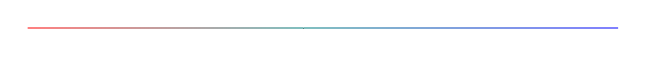
\begin{tikzpicture}
	\fill [left color=red!50, right color=teal!50] (0,0) rectangle (3.5,.01);
	\fill [left color=teal!50, right color=blue!50] (3.5,0) rectangle (7.5,.01);
	\end{tikzpicture}
\vspace{0.3cm}



\begin{ejercicio}
Calcula $\qquad <\, x \ > \ \text { y } \  <\, x^2 \ >	$
\end{ejercicio}
\vspace{5mm}

\color{MidnightBlue}

De la ecuación \ref{ApendicesIntegralGaussiana2}, $\ \displaystyle \int_{-\infty}^{+\infty} e^{-ax^2}\, \dd x \ =   \ \sqrt{\dfrac \pi a} \, , \  $ particularizando para $\ a \to \ a/2 \ $ tenemos:

$\displaystyle \boldsymbol{ \int_{-\infty}^{+\infty} e^{-(a/2)x^2}\, \dd x \ = }  \ \sqrt{\dfrac \pi {a/2}} \boldsymbol{ \ = \ \sqrt{ \dfrac{2\pi}{a} } }\, , \ $ expresión que nos servirá para todos los denominadores de los cálculos a efectuar.

\vspace{5mm} $\boldsymbol \triangleright \qquad $ Promedio de $x\, :  \qquad <\, x\, >=  \dfrac
{\displaystyle \int_{-\infty}^{+\infty} \dd x \, x\, e^{-\dfrac a 2 \, x^2}}
{\displaystyle \int_{-\infty}^{+\infty} \dd x \, e^{-\dfrac a 2 \, x^2}} $

La función que aparece en el integrando del numerador es una función \emph{impar}:

$f(x)=x\, e^{-\dfrac a 2 \, x^2} \quad \to \quad f(-x)=(-x)\, e^{-\dfrac a 2 \, (-x)^2}=-x\, e^{-\dfrac a 2 \, x^2}=-f(x)\, : \quad $ impar.

La integral de una función impar en un intervalo simétrico respecto del cero valo $0$, por lo que:

\begin{equation}
\label{Promedio-x}
\boldsymbol{ \boxed{ \ 
<\, x\, > \ = \ 0
\ } }	
\end{equation}

\begin{figure}[H]
	\centering
	\includegraphics[width=0.95\textwidth]{imagenes/apendices-01-09.png}
\end{figure}

Como consecuencia, podemos afirmar que el valor promedio de cualquier función impar también será cero:

\begin{equation}
\label{Promedio-x-impar}
\boldsymbol{ \ \boxed { \ 
<\, x^{2n+1}\, > \ = \ 0
\ } \ }	
\end{equation}

\begin{figure}[H]
	\centering
	\includegraphics[width=1\textwidth]{imagenes/apendices-01-10.png}
\end{figure}


\vspace{5mm} $\boldsymbol \triangleright \ \triangleright \qquad $ Promedio de $x^2\, :  \qquad <\, x^2\, >=  \dfrac
{\displaystyle \int_{-\infty}^{+\infty} \dd x \, x^2\, e^{-\dfrac a 2 \, x^2}}
{\displaystyle \int_{-\infty}^{+\infty} \dd x \, e^{-\dfrac a 2 \, x^2}} $

El denominador lo hemos calculado al principio del ejercicio y, de la misma forma, para el numerador aprovechamos el calculo de la ecuación \ref{ApendicesIntegralGaussiana3}
$\ \displaystyle  \int_{-\infty}^{+\infty} e^{-ax^2}\, x^2 \, \dd x  \ = \ \dfrac{\sqrt{\pi}}{2\, a^{3/2}} \, , \ $ sin más que cambiar $\ a \ \to \ a/2$

$\displaystyle \int_{-\infty}^{+\infty} e^{-(a/2)x^2}\, x^2 \, \dd x  \ = \ \dfrac{\sqrt{\pi}}{2\, (a/2)^{3/2}} =\dfrac{\sqrt{2\pi}}{a^{3/2}}$

Luego $\quad <\, x^2 \, > \ = \ \dfrac { \dfrac{\sqrt{2\pi}}{a^{3/2}} }{ \sqrt{ \dfrac{2\pi}{a} }  } \ = \ \dfrac 1 a$



\begin{equation}
\label{Promedio-x2}
\boldsymbol{ \boxed{ \ 
<\, x^2\, > \ = \ \dfrac{1}{a}
\ } }	
\end{equation}

\color{black}

\vspace{10mm}
\begin{ejercicio}
Comprueba que $\qquad <\, x^{2n} \, > \ = \ \dfrac 1{a^n} \, (2n-1)(2n-3)(2n-5) \cdots 5\cdot 3 \cdot 1 $
\end{ejercicio}
\vspace{5mm}

\color{MidnightBlue}

Vamos a, usando el mismo truco de derivar el integral gaussiana respecto del parámetros $a$, encontrar $\ <\, x^{4} \, >$

$\displaystyle \dv[2]{a}  \int_{-\infty}^{+\infty} e^{-ax^2} \, \dd x = \dv{a}  \int_{-\infty}^{+\infty} - x^2 \, e^{-ax^2} \, \dd x =  \int_{-\infty}^{+\infty} x^4 e^{-ax^2}\, \dd x = (\to)$

$\displaystyle (\to)= \dv[2]{a} \left( \sqrt{\dfrac \pi a} \right) = \dv[2]{a} (\sqrt{\pi} a^{-1/2} ) = \dv{a} (-1/2) \sqrt{\pi} a^{-3/2} = (-1/2)(-3/2)\sqrt{\pi} a^{-5/2}=\dfrac {3\pi}{4a^{5/2}}$

Tenemos $ \displaystyle \int_{-\infty}^{+\infty} x^4 e^{-ax^2}\, \dd x = \dfrac {3\pi}{4a^{5/2}} \, , \ $ haciendo el cambio $\ a \to \ a/2 $

$ \displaystyle \int_{-\infty}^{+\infty} x^4 e^{-(a/2)x^2}\, \dd x = \dfrac {3\pi}{4(a/2)^{5/2}} = \dfrac {3\sqrt{2\pi}}{a^{5/2}}$

Como para el cálculo del valor promedio todos los denominadores, como hemos visto al principio del ejercicio,  son  $\ \sqrt{\dfrac{2\pi}{a}}\, , \ $ tendremos:

$$\boldsymbol {  <\, x^4\, > \ = }\ \dfrac{\dfrac {3\sqrt{2\pi}}{a^{5/2}}}{\sqrt{\dfrac{2\pi}{a}}}\ = \boldsymbol { \ \dfrac 3 {a^2} }$$

\vspace{5mm} Intentemos generalizar este resultado:

$\boldsymbol{ \triangleright } \qquad \displaystyle \dv[n]{a} (e^{-ax^2})=(-x^2)^n e^{-ax^2}=(-1)^n x^{2n} e^{-ax^2} \quad \to \quad \dv[n]{a} \int_{-\infty}^{+\infty}  e^{-ax^2} \, \dd x = (-1)^n \,\int_{-\infty}^{+\infty} x^{2n} e^{-ax^2}\, \dd x $


$\boldsymbol{ \triangleright } \qquad \displaystyle \dv[n]{a}(\sqrt{\pi}a^{-1/2})=\sqrt{\pi} \left[ -\dfrac 1 2 \left(-\dfrac 1 2 - 1 \right) \left(\dfrac 1 2 - 2 \right) \cdots \left( -\dfrac 1 2 -(n-1) \right) \right] \, a^{-\dfrac 1 2 - n}=$

$= \sqrt{\pi} \left[  (-1)^n \dfrac 1 2 \dfrac 3 2 \dfrac 5 2 \cdots \dfrac {2n-1}2 \right] \, a^{-\dfrac 1 2 - n} = \sqrt{\dfrac \pi a } \, \left( \dfrac {-1}{2} \right)^n\, 1\cdot 3 \cdot 5 \cdot \cdots \cdot (2n-1) \, \dfrac 1 {a^n} $

Igualando los resultados obtenidos en los dos cálculos anteriores ($\triangleright$):

$\quad \displaystyle \cancel{(-1)^n} \, \int_{-\infty}^{+\infty} x^{2n} e^{-ax^2}\, \dd x  \ = \  \sqrt{\dfrac \pi a } \, \cancel{(-1)^n} \, \left( \dfrac {1}{2a} \right)^n\, 1\cdot 3 \cdot 5 \cdot \cdots \cdot (2n-1) $

Haciendo el cambio de siempre, $\ a \ \to \ a/2 \, , \ $

$\displaystyle  \int_{-\infty}^{+\infty} x^{2n} e^{-(a/2)x^2}\, \dd x  \ = \  \sqrt{\dfrac \pi {a/2} } \,  \left( \dfrac {1}{2(a/2)} \right)^n\, 1\cdot 3 \cdot 5 \cdot \cdots \cdot (2n-1)= \sqrt{\dfrac{2\pi}{a}} \dfrac 1 {a^n} \, 1\cdot 3 \cdot 5 \cdot \cdots \cdot (2n-1) $

Por último, al dividir esta integral por la que aparece en el denominador de todos los valores promedio,

$<\, x^{2n} \, > \ = \ \dfrac {\sqrt{\dfrac{2\pi}{a}} \, \dfrac 1 {a^n} \, 1\cdot 3 \cdot 5 \cdot \cdots \cdot (2n-1)}{\sqrt{\dfrac{2\pi}{a}}}  \ = \ \dfrac { 1\cdot 3 \cdot 5 \cdot \cdots \cdot (2n-1)}{a^n}$


\begin{equation}
\label{promedio-x2n}	
\boldsymbol{ \boxed{ \ 
<\, x^{2n} \, > \ = \  \dfrac { 1\cdot 3 \cdot 5 \cdot \cdots \cdot (2n-1)}{a^n}
\ } }
\end{equation}


\color{black}


%%%%%%%%%%%%%%%%%%%%%%%%%%%%%%%%%%%%%%%%%%%%%%%%

\chapter{?`Qué es un tensor}


\texttt{Apuntes basados en el video de Javier García, ``AULA 141 - DIRECTO: ?Qué es un TENSOR?''} 

 \rightline{ \textcolor{blue}{\textsf{\footnotesize{https://www.youtube.com/channel/UCYOv9HwOFwK0lY2dUQlZSpg}}} }


\begin{cita}{Javier García.}
``Un tensor es una extensión del concepto de vector, no de matriz''.

``No se puede ir por la vida sin saber lo que es un tensor''
\end{cita}

\section{Notación tensorial y convenio de Einstein}


\normalsize{Los} escalares son entes matemáticos que tienen 0-índices, los vectores tienen 1-índice, los tensores tendrán varios índices.


\begin{multicols}{2}
	\begin{figure}[H]
		\centering
		\includegraphics[width=.45\textwidth]{imagenes-tensores/tensor01.png}
	\end{figure}
	\begin{figure}[H]
		\centering
		\includegraphics[width=.5\textwidth]{imagenes-tensores/tensor02.png}
	\end{figure}
\end{multicols}

Comencemos con un vector $\overrightarrow{A}$ expresado en dos bases $\boldsymbol{B}=\{\vec e_1, \vec e_2\} \text{ y } \boldsymbol{B'}=\{\vec e_{1'}, \vec e_{2'}\}$. $A^1 \text { y } A^2$ serán las componentes de $\overrightarrow A$ en $\boldsymbol B$ y  $A^{1'} \text { y } A^{2'}$ serán las componentes de $\overrightarrow A$ en $\boldsymbol B'$ , es decir, 

$$ \text{En } B:\quad \overrightarrow A \ = \  A^1 \vec e_1 + A^2 \vec e_2;  \qquad \qquad \text{En } B':\quad  \overrightarrow A \ = \  A^{1'} \vec e_{1'} + A^{2'} \vec e_{2'} $$

Como, evidentemente, estamos hablando del mismo tensor:

$$\subrayado{\  \overrightarrow A \ = \  A^1 \vec e_1 + A^2 \vec e_2 \ \boldsymbol{=}\ A^{1'} \vec e_{1'} + A^{2'} \vec e_{2'} \ }$$ 	

\textcolor{gris}{Esta relación la ha de cumplir cualquier cosa que se quiera considerar vector o tensor, llevado a sus últimas consecuencias podría incluso servir como definición de tensor.}

\textcolor{gris}{En lo sucesivo, superíndices representarán componentes y subíndices vectores, con lo que nos ahorraremos las flechitas.}

Para cambiar de base, la relación entre componentes ha de ser lineal, por ello ha de existir una matriz $M$, con $\mathrm{det}\  M\neq 0$, para que la relación de cambio sea biunívoca, de modo que para componentes y vectores se cumpla:

$$\textcolor{red}{\left( \begin{matrix} A^{1'} \\ A^{2'} \end{matrix} \right)= M \left( \begin{matrix} A^{1} \\ A^{2} \end{matrix} \right)} \qquad \qquad { y } \qquad \qquad 
\textcolor{blue}{\left( \begin{matrix} e_{1'} \\ e_{2'} \end{matrix} \right)= {(M^{-1})}^T \left( \begin{matrix} e_{1} \\ e_{2} \end{matrix} \right)}$$


\begin{proof}
Veamos que si $M$ es la matriz de cambio de base que pasa de $B$ a $B'$ para las componentes, para los vectores	la matriz de cambio de base ha de ser ${(M^{-1})}^T$.


$$A^1e_1+A^2e_2 = ( e_1 \ e_2) \left( \begin{matrix} A^{1} \\ A^{2} \end{matrix} \right)  = 
\textcolor{blue}{ ( e_1 \ e_2) \ M^{-1}} \ \textcolor{red}{ M \ \left( \begin{matrix} A^{1} \\ A^{2} \end{matrix} \right)} = \textcolor{blue}{ ( e_{1'} \ e_{2'})} \ \textcolor{red} { \left( \begin{matrix} A^{1'} \\ A^{2'} \end{matrix} \right) }$$

Si esto es cierto, ocurrirá que $\quad \overrightarrow A \text{ en }B:\quad 
( e_1 \ e_2) \left( \begin{matrix} A^{1} \\ A^{2} \end{matrix} \right)
\ \boldsymbol{=} \ 
( e_{1'} \ e_{2'}) \left( \begin{matrix} A^{1'} \\ A^{2'} \end{matrix} \right) \quad : \overrightarrow A \text{ en }B'$

\textcolor{gris}{(Hemos multiplicado en medio de la ecuación matricial anterior por $I=M^{-1}M$)} La parte roja forma parte de la definición del cambio de base de las componentes, veamos que el cambio de base para los vectores es como dice la parte azul de la ecuación anterior.

Hemos de demostrar que $\quad (e_{1'} \ e_{2'})=(e_{1} \ e_{2})M^{-1}$. Recordemos, para ello, que la transposición de  matrices no conmuta sino que ${(XY)}^T=Y^TX^T$, por lo que:
$\textcolor{blue}{ \  \left( \begin{matrix}  e_{1'} \\ e_{2'} \end{matrix} \right) = {(M^{-1})}^T \left(  \begin{matrix}  e_{1} \\ e_{2} \end{matrix} \right) }$
\end{proof}

Hasta ahora tenemos que:

$$\boldsymbol{ \subrayado{\  \left( \begin{matrix} A^{1'} \\ A^{2'} \end{matrix} \right)= M \left( \begin{matrix} A^{1} \\ A^{2} \end{matrix} \right) \ } } \qquad \qquad { y } \qquad \qquad 
\boldsymbol{ \subrayado{\  \left( \begin{matrix} e_{1'} \\ e_{2'} \end{matrix} \right)= {(M^{-1})}^T \left( \begin{matrix} e_{1} \\ e_{2} \end{matrix} \right) \ } }$$

Vamos a ver lo que ocurre con las componentes de las matrices $M$ y ${(M^{-1})}^T$ e introduciremos la notación tensorial standard y en convenio de Einstein (\emph{`en una expresión, subíndices repetidos se suman')}.
		
$$ M=\left( \begin{matrix}
 M^{1'}_{1} & M^{1'}_{2} \\ M^{2'}_{1} & M^{2'}_2	
 \end{matrix} \right)
 \qquad \to \qquad 
\left( \begin{matrix} A^{1'} \\ A^{2'} \end{matrix} \right)=
\left( \begin{matrix} M^{1'}_{1} & M^{1'}_{2} \\ M^{2'}_{1} & M^{2'}_{2}	
 \end{matrix} \right)
 \left( \begin{matrix} A^{1} \\ A^{2} \end{matrix} \right) $$
 
 Los índices de arriba, \emph{`superíndices'}, indican filas y los índices de abajo,  \emph{`subíndices'} indican columnas. La matriz  $M=( \ M^{i'}_j \ )$ pasa de componentes antiguas $A^k$ a componentes nuevas $A^{k'}$. Trabaja sobre objetos con superíndice, con el índice arriba, (componentes del vector).
 
 Por analogía: 
 
 $$
 \left( \begin{matrix} e_{1'} \\ e_{2'} \end{matrix} \right)=
\left( \begin{matrix} M^{1}_{1'} & M^{2}_{1'} \\ M^{1}_{2'} & M^{2}_{2'}	
 \end{matrix} \right)
 \left( \begin{matrix} e_{1} \\ e_{2} \end{matrix} \right)
 $$
 
Donde en ${(M^{-1})}^T$ hemos cambiado las primas de superíndices a subíndices y hemos traspuesto (cambiado filas por columnas)	:

$$	
M=\left( \begin{matrix}
 M^{1'}_{1} & M^{1'}_{2} \\ M^{2'}_{1} & M^{2'}_{2}	
 \end{matrix} \right) \quad \to \quad
 M^{-1}=\left( \begin{matrix}
 M^{1}_{1'} & M^{1}_{2'} \\ M^{2}_{1'} & M^{2}_{2'}	
 \end{matrix} \right) \quad \to \quad
 {(M^{-1})}^T=
 \left( \begin{matrix} M^{1}_{1'} & M^{2}_{1'} \\ M^{1}_{2'} & M^{2}_{2'}	\end{matrix} \right) $$
 
\begin{table}[H]
\centering
\begin{tabular}{ccc}
$\left( \begin{matrix} A^{1'} \\ A^{2'} \end{matrix} \right)= M \left( \begin{matrix} A^{1} \\ A^{2} \end{matrix} \right)$ & $\quad$ & $\left( \begin{matrix} e_{1'} \\ e_{2'} \end{matrix} \right)= {(M^{-1})}^T \left( \begin{matrix} e_{1'} \\ e_{2'} \end{matrix} \right)$  
\end{tabular}
\end{table}


\begin{table}[H]
\centering
\begin{tabular}{ccc}
 \multicolumn{3}{l}{Multiplicando:}     \\ 
$A^{1'}=M^{1'}_{1}A^1+M^{1'}_{2}A^2$                                                                                     & $\quad$ & $e_{1'}=M^{1}_{1'}e_1+M^{2}_{1'}e_2$                                                                                                  \\
$A^{2'}=M^{2'}_{1}A^1+M^{2'}_{2}A^2$                                                                                     & $\quad$ & $e_{2''}=M^{1}_{2'}e_1+M^{2}_{2'}e_2$ \\                                                                                        
\end{tabular}
\end{table}                                                                                   

 
 \begin{table}[H]
\centering
\begin{tabular}{ccc}
 \multicolumn{3}{l}{Usando el convenio de Einstein -índices repetidos se suman-: }     \\     
$\subrayado{\  \boldsymbol{ \boxed{\  A^{i'} =\textcolor{red}{M^{i'}_{j}} A^j \ } } \ }$ & $\quad$ & $\subrayado{\  \boldsymbol{ \boxed{\ e_{i'}=\textcolor{blue}{M^{j}_{i'}} e_{j} \ } } \ }$                                                                                          
\end{tabular}
\end{table}
 
 $M$ da el cambio de base de las componentes antiguas $A^i$ a las nuevas $A^{i'}$; ${(M^{-1})}^T$ da el cambio de base de los vectores antiguos $e_i$ a los nuevos $e_{i'}$.
 
 Con esta notación (tensorial) aumenta muchísimo la potencia de cálculo.
 
 Veamos una propiedad importante, como $ M^{-1} \ M =I$, tendremos, que cada elemento de este producto se obtendrá como suma de los productos de la fila-i de $ M^{-1}$ por la columna-j de $M$ (recordar que los subíndices son las filas y los superíndices las columnas de la matriz):
$M^{\textcolor{DarkGreen}{i'}}_{j}\ M^k_{\textcolor{DarkGreen}{i'}} \ = \ \delta^k_j \ = \ I^k_j $
 
$$\subrayado{ \  \boxed{\ \boldsymbol{M^{\textcolor{DarkGreen}{i'}}_{j}\ M^k_{\textcolor{DarkGreen}{i'}} \ = \ \delta^k_j } \ } \ }
 \qquad \text{donde } \delta^k_j=\begin{cases} 0 & \text{si } j\neq k \\ 1 & \text{si } j=k \end{cases} \text{ es la llamada \emph{\textbf{delta de Kronecker.}} }$$
 
Veamos la potencia de la notación tensorial:

$A^{i'} e_{i'}=M^{i'}_{j} A^j M^{k}_{i'} e_k = \text{\textcolor{gris}{(los números conmutan, las matrices no)}}=$

$= A^j M^{i'}_{j}M^{k}_{i'}e_k=A^j \delta ^k_j e_k=A^je_j$

y, en una sola línea, tenemos demostrado el motivo de todo lo que estamos haciendo: todo vector, aunque se exprese de distintas formas en distintas bases, siempre es el mismo vector.
 
\section{Producto Escalar}

\begin{table}[H]
\centering
\begin{tabular}{ll}
\multicolumn{2}{l}{\textbf{Propiedades del producto escalar $\overrightarrow A \cdot \overrightarrow B$}} \\
Linealidad por la izquierda              & $\quad (a\overrightarrow A \cdot +b\overrightarrow B)\cdot \overrightarrow C  = a\overrightarrow A \cdot \overrightarrow C + b \overrightarrow B \cdot \overrightarrow C$          \\
Linealidad por la derecha                & $\quad \overrightarrow A \cdot (b\overrightarrow B+c \overrightarrow C)=b\overrightarrow A \cdot \overrightarrow B + c \overrightarrow A \cdot \overrightarrow B$                                        \\
Conmutatividad, PE es Simétrico           & $\quad \overrightarrow A \cdot \overrightarrow B= \overrightarrow B \cdot \overrightarrow A$                  
\end{tabular}
\end{table}
 
 Llamaremos \emph{\textbf{métrica}} a los productos escalares de los vectores de la base: $\subrayado{ \ \boxed{ \boldsymbol{e_i \cdot e_j \ = \ g_{ij}} \ } \ }$
 
 \textbf{Expresión del producto escalar en forma matricial:}
 
 $\overrightarrow A \cdot \overrightarrow B = (A^1e_1+A^2e_2)\cdot (B^1e_1+B^2e_2)=A^1B^1e_1\cdot e_1 + A^1B^2 e_1\cdot e_2 + A^2B^1 e_2\cdot e_1 + A^2B^2 e_2\cdot e_2=$
 
 $=A^1B^1g_{11}+A^1B^2g_{12}+A^2B^1g_{21}+A^2B^2g_{22}$, matricialmente coincide con
 
 $$\boldsymbol{\overrightarrow A \cdot \overrightarrow B \ = \ \left( \begin{matrix}  A^1&A^2 \end{matrix} \right) \left( \begin{matrix} \ g_{11} & g_{12} \\ g_{21} & g_{22} \end{matrix} \right) \  \left( \begin{matrix} B^1 \\ B^2 \end{matrix} \right)}$$
 
 $$\text{De forma más compacta, } \qquad \subrayado{\ \boxed{\ \boldsymbol{ \overrightarrow A \cdot \overrightarrow B = A^T \ g \ B}\ }\ }$$
 
\textcolor{gris}{Las componentes de vectores se escriben como matrices columna, $A^T$ será matriz fila.} 
 
 \emph{?`Qué se puede hacer con el producto escalar?} $\ \to \ $ medir la longitud de un vector: $\quad \boldsymbol{ \norm{\overrightarrow A}=+\sqrt{\overrightarrow A \cdot \overrightarrow A} }$
 
 En cartesianas (BON \footnote{BON: base orto-normal}), $\ g_{ij}=\delta_{ij}=\begin{cases} 0 & \text{si } i\neq j \\ 1 & \text{si } i=j \end{cases}$,
 
 $ \norm{\overrightarrow A} = \sqrt{\left( \begin{matrix}  A^1&A^2 \end{matrix} \right) \left( \begin{matrix} \ 1 & 0 \\ 0 & 1 \end{matrix} \right) \  \left( \begin{matrix} A^1 \\ A^2 \end{matrix} \right)} =\sqrt{(A^1)^2+(A^2)^2}\ $ (Expresion sólo valida en una BON de un espacio plano. Se trata, en realidad, del teorema de Pitágoras.)
 
\section{Base Dual} 

\begin{resumen}
\vspace{-10mm}
\textcolor{gris}{\textbf{Nota para matemáticos:}}

\textcolor{gris}{Los matemáticos definen el espacio vectorial dual V* como funciones lineales que transforman vectores de V en escalares. No hay necesidad de definir un producto escalar. Pero en los casos en los que sí se ha definido un producto escalar en V, se genera de forma natural un isomorfismo entre V* y V inducido por la métrica.}

\textcolor{gris}{ Este isomorfismo permite una reformulación en la que los vectores duales ``conviven'' con los vectores en el mismo espacio V.}
\vspace{-10mm}
\begin{resumen} 
\textcolor{gris}{--- Los espacios vectoriales que aparecen en Relatividad General están dotados de una métrica, así que en lo que sigue adoptaremos este punto de vista.}

\textcolor{gris}{--- En Mecánica Cuántica, los vectores del espacio dual se puede representar como vectores fila conjugados y el producto escalar tiene como métrica la identidad.}
\end{resumen}
\end{resumen}

$B \text{ en } V:\ \{e_1,e_2\}$. A partir de ella, construimos una nueva base de vectores en $V*$, completamente distinta a esta, que llamaremos \emph{\textbf{base dual}}, $\{e^1,e^2\}$, de modo que:

$$\subrayado{ \ \boxed{ \ \boldsymbol{e^i\ e_j\ =\ \delta^i_j} \ } \ }$$

------ ?`Cómo podemos calcular estos vectores?:
$\quad \begin{matrix}
 e^1\ = \ ae_1 \ + \ be_2 \\ e^2 \ = \ ce_1	\ + \ d e_2
 \end{matrix}\ ; \qquad a,d,c,d\text{ incógnitas}
$

Imponiendo la condición, $\quad 1=e^1e_1=(e^1)^T\ g\ e_1=(a \ b ) \ g \  \left( \begin{matrix} 1 \\ 0 \end{matrix} \right) \ \to \ (*)$

\textcolor{gris}{Evidentemente, $\quad e_1=\left( \begin{matrix} 1 \\ 0 \end{matrix} \right)=1e_1+0e_2; \qquad  
e_2=\left( \begin{matrix} 0 \\ 1 \end{matrix} \right)=0e_1+1e_2$}

 Como $\quad (1, 0) \left( \begin{matrix} 1 \\ 0 \end{matrix} \right) = 1 \to \ (*):\ (a \ b) \ g = (1\ 0) \ (**)$, trasponiendo:
 
 $\left[ (a\ b) \ g \right]^T=g^T\ (a\ b)^T= g^T\ \left( \begin{matrix} a \\ b \end{matrix} \right) \ \ \boldsymbol{=} \  (**) \ \boldsymbol{=} \ \ (1\ 0)^T = \left( \begin{matrix} 1 \\ 0 \end{matrix} \right)$
 
 Tenemos que $\ g^T\ \left( \begin{matrix} a \\ b \end{matrix} \right) \ = \ \left( \begin{matrix} 1 \\ 0 \end{matrix} \right)$, 
 
 pero, al ser el producto escalar conmutativo (simétrico), la métrica también lo es: 
 
 $\boldsymbol{g=g^T} \quad (***)$, por lo que  
 
 $\ g\ \left( \begin{matrix} a \\ b \end{matrix} \right) \ = \ \left( \begin{matrix} 1 \\ 0 \end{matrix} \right)$.
 
 Premultiplicando ahora por $g^{-1}:\quad g^{-1} \ g \ \left( \begin{matrix} a \\ b \end{matrix} \right) = I \ \left( \begin{matrix} a \\ b \end{matrix} \right) = \left( \begin{matrix} a \\ b \end{matrix} \right) \ \boldsymbol{=} \ \ g^{-1} \ \left( \begin{matrix} 1 \\ 0 \end{matrix} \right) $
 
 Es decir, $\ \left( \begin{matrix} a \\ b \end{matrix} \right) = g^{-1} \ \left( \begin{matrix} 1 \\ 0 \end{matrix} \right) \ \ \boldsymbol{=} \ \ e^1 \ $, ya que $\ \ e^i\ e_j=\delta^i_j$
 
 Llamando $g^{ij}$ a los elementos de la inversa de la métrica \textcolor{gris}{$\left[ g=(g_{ij});\ g^{-1}=(g^{ij}) \right]$}, tenemos
 
 $\left( \begin{matrix} a \\ b \end{matrix} \right)=
 \left( \begin{matrix} g^{11}&g^{12} \\ g^{21}&g^{22} \end{matrix} \right)
 \left( \begin{matrix} 1 \\ 0 \end{matrix} \right)
 =\left( \begin{matrix} g^{11} \\ g^{21} \end{matrix} \right)
 \quad \to \quad a=g^{11};\ \ b=g^{21}$
 
 de donde, $\ e^1=ae_1+be_2=g^{11}e_1+g^{21}e_2$
 
 Al ser tanto $g$ como $g^{-1}$ simétricas, se cumple que $\ g^{21}=g^{12} $, 

entonces $\ e^1=g^{11}e_1+g^{12}e_2$, por el convenio de Einstein, $\ e^1=g^{1j}e_j$ y, análogamente, $e^2=g^{2j}e_j$.

De forma compacta, 

$$ \subrayado{ \ \boxed{ \ \boldsymbol{ e^i \ = \ g^{ij} \ e_j} \ } \ }
% \qquad \qquad \textcolor{gris}{
% \left( \begin{matrix} e^1\\e^2 \end{matrix} \right) =
% \left( \begin{matrix} g^{11}&g^{12}\\g^{21}&g^{22} \end{matrix} \right)
% \left( \begin{matrix} e_1\\e_2 \end{matrix} \right) }
$$

------ ?`Cuáles serán las componentes duales, $A_i$, para que el vector sea invariante? 

\textcolor{gris}{$\qquad \overrightarrow A=A^1e_1+A^2e_2=A^{1'}e_{1'}+A^{2'}e_{2'}=A_1e^1+A_2e^2$}

Vamos a hacerlo usando que $ e^i \ = \ g^{ij} \ e_j$ y la notación tensorial.

$A_i{\textcolor{red}{e^i}}=A_i {\textcolor{red}{g^{ij}e_j}} \equiv A^je_j$, esto el lo que queremos que ocurra. Para ello, como el producto de números conmuta, $\ A^j=g^{ij}A_i$

Como $g^{ij}$ son los elementos de $g^{-1}$, premultiplicando por $g$,
$\ \textcolor{blue}{g_{kj}}A^j=\textcolor{blue}{g_{kj}}g^{ji}A_i \ $ \textcolor{gris}{Para multiplicar matrices, ha de haber un índice abajo y otro, repetido, arriba. El grado libre de arriba da como resultado un vector}.

$g_{kj}g^{ji} \to gg^{-1} \to I \to \delta_k^j \quad \to \quad \boldsymbol {g_{kj}A^j=A_k} \qquad \qquad \qquad \qquad \Box$ 

$$\textbf{Resumen:} \qquad \qquad  \qquad \qquad  \qquad \subrayado{ \ \boxed{ \ \boldsymbol{ e^i \ = \ g^{ij} \ e_j} \ } \ }  \qquad \leftrightarrow \qquad 
\subrayado{ \ \boxed{ \ \boldsymbol{ A_i \ = \ g_{ij} \ A^j} \ } \ }$$ 

\begin{center}
	\colorbox{LightYellow}{\textcolor{DarkBlue}{\emph{\textbf{ !`El famoso subir y bajar de índices! }}}}
\end{center}

\textcolor{gris}{Demostremos que, al ser el producto escalar conmutativo, $\overrightarrow A \cdot \overrightarrow B = \overrightarrow B \cdot \overrightarrow A$ , entonces la métrica es simétrica, $g^T=g$}

\textcolor{gris}{
$\overrightarrow A \cdot \overrightarrow B=A^T\ g \ B;\quad \overrightarrow B \cdot \overrightarrow A=B^T\ g\ A \quad \to \quad A^T \ g \ B = B^T \ g \ A.\ $ El traspuesto de un número es él mismo:
}

\textcolor{gris}{
$A^T\ g \ B = (A^T \ g B)^T = (A^T \ (gB))^T = (gB)^T \ (A^T)^T= B^T \ \underline{g^T} \ A\  $ que, por la comuntatividad de PE es igual a $\ B^T\ \underline{g} \ A$, por lo que, necesariamente, $\ \boldsymbol{g=g^T} \  \qquad \qquad \qquad \qquad \Box$ 
} 

Cuando las componentes de un vector tienen los índices arriba, super-índices, se les llama \textbf{componentes \textsf{CONTRAVARIANTES}}, $\boldsymbol{A^i}$, cuando tienen las componentes abajo, sub-índices, se les llama \textbf{componentes \textsf{COVARIANTES}}, $\boldsymbol{A_i}$.

\subsection{?`Cómo se transforma la métrica ante un cambio de base?}

Exigiremos que el producto escalar de dos vectores dé el mismo resultado independientemente de la base en que estén expresados ambos vectores, lo cual es obvio, la longitud de un vector ha de ser independiente de la base en que éste se exprese. 

Lo haremos con notación tensorial:

$\overrightarrow A\cdot \overrightarrow B = \textcolor{gris}{(A^T\ g \ B)} = $
$=\textcolor{DarkGreen}{\boldsymbol{g_{ij}A^iB^j}}=\textcolor{gris}{(g_{11}A^1B^1+g_{12}A^1B^2+\cdots)}=g_{ij}A^{\textcolor{red}{i}}B^{\textcolor{red}{j}}= $

hacemos el cambio de base:

$=g_{\textcolor{red}{ij}}M_{{\textcolor{blue}{j'}}}^{\textcolor{red}{i}}A^{\textcolor{blue}{j'}}M_{\textcolor{blue}{k'}}^{\textcolor{red}{j}}B^{\textcolor{blue}{k'}}=$

\textcolor{gris}{($M_{j'}^{i}$ es la matriz inversa del cambio de base, las primas están abajo, cambian de nuevo, $A^{j'}$, a viejo, $A^i$). En esta expresión lo que aparece son números, conmutan, podemos reordenarlos.)}

$=\boxed{\boldsymbol{M_{j'}^{i}M_{k'}^{j} g_{}ij}}\ A^{j'}B^{k'}=$

para que coincida con $\overrightarrow A\cdot \overrightarrow B$ en la nueva base, esta expresión ha de ser igual a

$=\textcolor{DarkGreen}{\boldsymbol{\boxed{g_{j'k'}} \ A^{j'}B^{k'}}}$

por lo que: $\quad g_{j'k'}=M_{j'}^{i}M_{k'}^{j} g_{}ij$, o, renombrando los índices (mudos j' y k'),

$$\boldsymbol{g_{i'j'}\ = \ M_{j'}^{i} \ M_{k'}^{j} \ g_{}ij} $$

\begin{center}
	\colorbox{LightYellow}{\textcolor{DarkBlue}{\emph{\textbf{ !`Esto es un ejemplo de lo que va a ser un \textsw{tensor}! }}}}
\end{center}

\section{Ejemplo numérico}

Sea $\{ e_1,e_2 \}$ una base de un espacio vectorial $V$ y sea $g_{ij}=\left( \begin{matrix} g_{11} & g_{12} \\ g_{21} & g_{22} \end{matrix} \right) = \left( \begin{matrix} 5&-2\\-2&8 \end{matrix} \right)$ la métrica en este espacio (es simétrica y con determinante no nulo).

Tomemos un vector $\ \overrightarrow A = 4e_1+2e_2,\ $ sus componentes son $\ A^1=4;\ A^2=2$.

------ Vamos a hacer un \underline{cambio a otra base} $\{ e_{1'},e_{2'} \},\ $ de modo que la matriz de este cambio de base sea: 

$\ M=\left( \begin{matrix} M_1^{1'} & M_2^{1'} \\ M_1^{2'} & M_2^{2'} \end{matrix} \right)=
\left( \begin{matrix} 1&3\\5&7 \end{matrix} \right)$ 

\textcolor{gris}{superíndices=filas; subíndices=columnas. Las primas están arriba (superíndices), por ello $M$ pasa de vectores viejos (sin primas, $e_k$) a vectores nuevos (con primas $e_{l'}$), $M$ es la matriz que cambia de la base vieja, $\{ e_1,e_2 \}$, a la nueva,  $\{ e_{1'},e_{2'} \}.$}

Cálculos matriciales: $\quad M=
\left( \begin{matrix} 1&3\\5&7 \end{matrix} \right)
\quad \to \quad 
{(M^{-1})}^T=
\left( \begin{matrix} -\dfrac 7 8& \dfrac 5 8 \\ \dfrac 3 8 & - \dfrac 1 8 \end{matrix} \right)=
\left( \begin{matrix} M_{1'}^{1} & M_{1'}^{2} \\ M_{2'}^{1} & M_{2'}^{2} \end{matrix} \right)$

\textcolor{gris}{${(M^{-1})}^T$, por ser inversa, las primas van abajo; por ser traspuesta, hemos cambiado filas por columnas.}

\begin{multicols}{2}
	
La relación entre las dos bases será:

$\quad$

$ \left( \begin{matrix} e_{1'} \\ e_{2'} \end{matrix} \right) =
{(M^{-1})}^T \ 
\left( \begin{matrix} e_{1} \\ e_{2} \end{matrix} \right) \quad \to \quad \begin{cases}
	\ e_{1'}=- \dfrac 7 8 e_1 + \dfrac 5 8 e_2 \\ 
	\ e_{2'}=  \ \ \dfrac 3 8 e_1 - \dfrac 1 8 e_2
\end{cases}$


	\begin{figure}[H]
		\centering
		\includegraphics[width=.3\textwidth]{imagenes-tensores/tensor03.png}
	\end{figure}

\end{multicols}

------ Veamos cuales son las \underline{componentes del vector $\overrightarrow A$ en la nueva base}.

$\left( \begin{matrix} A^{1'} \\ A^{2'} \end{matrix} \right) =
M\ \left( \begin{matrix} A^{1} \\ A^{2} \end{matrix} \right)=
\left( \begin{matrix} 1&3\\5&7 \end{matrix} \right) \ 
\left( \begin{matrix} 4 \\ 2 \end{matrix} \right)=
\left( \begin{matrix}10 \\ 34 \end{matrix} \right). \quad$
Luego, $\ \overrightarrow A\ =\  4e_1+2e_2 \ = \ 10e_{1'}+34e_{2'}$

------ Cálculo de la \underline{base dual}:

$g_{ij}=\left( \begin{matrix} g_{11} & g_{12} \\ g_{21} & g_{22} \end{matrix} \right) = \left( \begin{matrix} 5&-2\\-2&8 \end{matrix} \right)$
$\quad \to \qquad$
$g^{ij}=\left( \begin{matrix} g^{11} & g^{12} \\ g^{21} & g^{22} \end{matrix} \right) = \left( \begin{matrix} 5&-2\\-2&8 \end{matrix} \right)^{-1}=
\left( \begin{matrix} \dfrac 2 9&\dfrac 1 {18}\\\dfrac 1 {18}&\dfrac 5{36} \end{matrix} \right)$

matriz dual de la métrica que, evidentemente, también es simétrica.

Recordando la definición de espacio dual:

$e^1=g^{1j}e_j=g^{11}e_1+g^{12}e_2=\dfrac 2 9 e_1+\dfrac 1 {18} e_2$
$;\qquad$
$e^2=g^{2j}e_j=g^{21}e_1+g^{22}e_2=\dfrac 1 {18} e_1+\dfrac 5 {36} e_2$

\begin{multicols}{2}
	Podemos, al contrario que los matemáticos y porque nuestro espacio tiene una métrica, representar los vectores y sus duales en el mismo plano. Si no tuviéramos métrica, $e^1 \text{ y } e^2$ serían funciones multilineales y `vivirían' en otro espacio, $V^*$.

	\begin{figure}[H]
		\centering
		\includegraphics[width=.3\textwidth]{imagenes-tensores/tensor04.png}
	\end{figure}
\end{multicols}

------ Vamos a comprobar que se cumple la \underline{condición de la base dual}: $\boldsymbol{e^i \cdot e_j=\delta^i_j}$

$1=\delta^1_1=e^1\cdot e_1=(e^1)^T\ g \ e_1 = 
\left( \begin{matrix} \dfrac 2 9 & \dfrac 1 {18} \end{matrix} \right)
\left( \begin{matrix} 5&-2\\-2&8 \end{matrix} \right)
\left( \begin{matrix} 1 \\ 0 \end{matrix} \right) = 1,\quad 0K!$

$0=\delta^1_2=e^1\cdot e_2=(e^1)^T\ g \ e_2 = 
\left( \begin{matrix} \dfrac 2 9 & \dfrac 1 {18} \end{matrix} \right)
\left( \begin{matrix} 5&-2\\-2&8 \end{matrix} \right)
\left( \begin{matrix} 0 \\ 1 \end{matrix} \right) = 0,\quad 0K!$

$0=\delta^2_1=e^2\cdot e_1=(e^2)^T\ g \ e_1 = 
\left( \begin{matrix} \dfrac 1 {18} & \dfrac 5 {36} \end{matrix} \right)
\left( \begin{matrix} 5&-2\\-2&8 \end{matrix} \right)
\left( \begin{matrix} 1 \\ 0 \end{matrix} \right) = 0,\quad 0K!$

$1=\delta^2_2=e^2\cdot e_2=(e^2)^T\ g \ e_2 = 
\left( \begin{matrix} \dfrac 1 {18} & \dfrac 5 {36} \end{matrix} \right)
\left( \begin{matrix} 5&-2\\-2&8 \end{matrix} \right)
\left( \begin{matrix} 0 \\ 1 \end{matrix} \right) = 1,\quad 0K!$

------ Ahora, vamos a calcular las \underline{componentes duales del vector}  $\overrightarrow A$ :\textcolor{gris}{$\quad (A_i=g_{ij}A^j)$}

\begin{multicols}{2}
$\quad$
	
$A_1=g_{1j}A^j=g_{11}A^1+g_{12}A^2=$

$\quad \ \ =5A^1-2A^2=5\cdot 4-2\cdot 2=16$

$A_2=g_{2j}A^j=g_{21}A^1+g_{22}A^2=$

$\quad \ \ =-2A^1+8A^2=-2\cdot 4+8\cdot 2=8$

Luego, $\ \overrightarrow A=16e^1+8e^2$

\begin{figure}[H]
		\centering
		\includegraphics[width=.2\textwidth]{imagenes-tensores/tensor05.png}
	\end{figure}
	
\end{multicols}
	
\textcolor{gris}{Matricialmete:}

\textcolor{gris}
{$
\left( \begin{matrix} A_1\\A_2 \end{matrix} \right)=
\left( \begin{matrix} g_{11} & g_{12} \\ g_{21} & g_{22} \end{matrix} \right)
\left( \begin{matrix} A^1 \\ A^2 \end{matrix} \right) =
\left( \begin{matrix} 5 & -2 \\ -2 & 8 \end{matrix} \right)
\left( \begin{matrix} 4 \\ 2 \end{matrix} \right) =
\left( \begin{matrix} 16 \\ 8 \end{matrix} \right) 
$}

------ Comprobemos que, efectivamente, lo encontrado \underline{describe el mismo vector} $\overrightarrow A$.

$\overrightarrow A=16e^1+8e^2=16 \left(\dfrac 2 9 e_1+\dfrac 1 {18} e_2 \right) + 8 \left( \dfrac 1 {18} e_1+\dfrac 5 {36} e_2 \right)=4e_1+2e_2,\quad OK!$

------ \underline{Cambio de base de la métrica}, matricialmente: (ya no estamos en la base dual, estamos ante un cambio de base de vectores `normales', de $\{e_1,\ e_2\}$ a $\{e_{1'},\ e_{2'}\}$).

\begin{multicols}{2}
$$\boldsymbol{ g'\ = \ (M^T)^{-1} \ g \ M^{-1} } \qquad \textcolor{gris}{\text{(no demostrado)}}$$

	\begin{figure}[H]
		\centering
		\includegraphics[width=.25\textwidth]{imagenes-tensores/tensor06.png}
	\end{figure}
\end{multicols}



$g_{ij}= \left( \begin{matrix} 5&-2\\-2&8 \end{matrix} \right)$
$; \ \ $
$M=\left( \begin{matrix} 1&3\\5&7 \end{matrix} \right)$
$ \quad \to \quad $ 
$g_{i'j'}=\left[  \left( \begin{matrix} 1&3\\5&7 \end{matrix} \right)^T   \right]^{-1}
\left( \begin{matrix} 5&-2\\-2&8 \end{matrix} \right)
\left( \begin{matrix} 1&3\\5&7 \end{matrix} \right)^{-1}=
\left( \begin{matrix} \dfrac{585}{64}&\dfrac{-189}{64}\\\dfrac{-189}{64}&\dfrac{65}{64} \end{matrix} \right)$

Si en vez de matricialmente lo hacemos componente a componente aplicaremos la fórmula $\ \boldsymbol{ g_{i'j'}=M^i_{i'}M^j_{j'}g_{ij} } ,\ $
\textcolor{gris}{\text{(esto sí lo vimos.)}}

$g_{ij}= \left( \begin{matrix} 5&-2\\-2&8 \end{matrix} \right)$
$; \ \ $
$M^{-1}=\left( \begin{matrix} M^1_{1'}&M^1_{2'}\\M^2_{1'}&M^2_{2'} \end{matrix} \right)=
\left( \begin{matrix} -\dfrac 7 8&\dfrac 3 8\\\dfrac 5 8&-\dfrac 1 8 \end{matrix} \right)\quad $ \textcolor{gris}{(las primas en $M$ están abajo: es $M^{-1}$)}

Calculemos elemento a elemento.

$g_{1'1'}=M^1_{1'}M^1_{1'}g_{11}+M^1_{1'}M^2_{1'}g_{12}+M^2_{1'}M^1_{1'}g_{21}+M^2_{1'}M^2_{1'}g_{22}=$

$\quad = -\dfrac 7 8 \left( -\dfrac 7 8\right) 5 + (-\dfrac 7 8) \dfrac 5 8 (-2)+ \dfrac 5 8 \left( - \dfrac 7 8 \right) (-2) + \dfrac 5 8 \dfrac 5 8 8\ \  =\ \  \dfrac{585}{64}$

$g_{1'2'}=
M^1_{1'}M^1_{2'}g_{11}+M^1_{1'}M^2_{2'}g_{12}+M^2_{1'}M^1_{2'}g_{21}+M^2_{1'}M^2_{2'}g_{22}=$

$\quad = \left( - \dfrac 7 8 \right) \dfrac 3 8 5 + \left( -\dfrac 7 8 \right) \left(-\dfrac 1 8 \right) (-2) + \dfrac 5 8 \dfrac 3 8 (-2) + \dfrac 5 8 \left( - \dfrac 1 8  \right) 8 \  = \  -\dfrac{189}{64}$

Haciendo los dos cálculos que faltan y completando, obtenemos, $\ g_{i'j'}=\left( \begin{matrix} \dfrac{585}{64}&\dfrac{-189}{64}\\\dfrac{-189}{64}&\dfrac{65}{64} \end{matrix} \right)$

Resultado que, como era de esperar, coincide con el encontrado matricialmete.

------ \underline{El producto escalar es invariante bajo cambios de base}. 

\begin{multicols}{2}
\textcolor{gris}{Como tiene que ser, el producto escalar de un vector por sí mismo mide la longitud del vector y ello no puede depender de la base en que éste se exprese.}

Veámoslo con un ejemplo: 

$\overrightarrow A=4e_1+2e_2$

$\overrightarrow B=-3e_1+5e_2$

\begin{figure}[H]
		\centering
		\includegraphics[width=.25\textwidth]{imagenes-tensores/tensor07.png}
	\end{figure}
\end{multicols}


	
$\overrightarrow A\cdot \overrightarrow B=(A)^T\ g \ (B)=\mqty(4&2) \mqty(5&-2\\-2&8) \mqty(-3\\5) =\mqty(16&8) \mqty(-3\\5)=-8$

\textcolor{gris}{OJO: $\quad \overrightarrow A\cdot \overrightarrow B=4(-3)+2(5)=-12+10=-2 \ \leftrightarrow \ g_{ij}= \mqty(1&0\\0&1)$ }

Averiguamos las componentes de $\overrightarrow A \text{ y } \overrightarrow B$ en $\{e_{1'},\ e_{2'}\}$ usando la matriz de cambio $M$

$\mqty(1&3\\5&7) \mqty(4\\2) = \mqty(10\\34) \to \overrightarrow A=10e_{1'}+34e_{2'}$
$;\qquad$
$\mqty(1&3\\5&7) \mqty(-3\\5) = \mqty(12\\20) \to \overrightarrow B=12e_{1'}+20e_{2'}$

Calculamos el producto escalar con la nueva métrica, matricialmente:

$\overrightarrow A \cdot \overrightarrow B = (A^T) \ g_{i'j'} \ (B)=
\mqty(10&34) \mqty(\dfrac{584}{64}&-\dfrac{189}{64}\\-\dfrac{189}{64}&\dfrac{65}{64}) \mqty(12\\20) \ = \ -8,\quad OK!$

\textcolor{gris}{------ ?`También será \underline{invariante el producto escalar en la base dual}?}

\textcolor{gris}{$\overrightarrow A \cdot \overrightarrow B = (A_{cov})^T\ g^{ij}\ (B_{cov});\qquad g^{ij}=\mqty(\dfrac 2 9 & \dfrac 1 {18} \\ \dfrac 1 {18} & \dfrac 5 {36})$}

\textcolor{gris}{$\overrightarrow A_{cov}=\mqty(A^1\\A^2)=\mqty(16\\8)$}

\textcolor{gris}{$\overrightarrow B_{cov}=\mqty(B^1\\B^2)=\mqty(g_{11}&g_{12}\\g_{21}&g_{22})\mqty(B^1\\B^2)= \mqty(5&-2\\-2&8)\mqty(-3\\5)=\mqty(-25\\46)$}

\textcolor{gris}{$\overrightarrow A \cdot \overrightarrow B = (A_{cov})^T\ g^{ij}\ (B_{cov})=\mqty(16&8) \mqty(\dfrac 2 9 & \dfrac 1 {18} \\ \dfrac 1 {18} & \dfrac 5 {36}) \mqty(-25\\46)\ =\ -8,\quad Super-OK!$}

\begin{center}
	\colorbox{LightYellow}{\textcolor{DarkBlue}{\emph{\textbf{ !`Ya estamos preparados para entender qué es un \textsw{tensor}! }}}}
\end{center}

\section{Definición de tensor}

A partir de cómo cambia la métrica bajo un cambio de base, definimos un ``tensor'' como una `entidad' con índices que transforma de la misma manera: $\ g_{i'j'}=M^i_{i'}M^j_{j'}g_{ij}$

$$\text{!`Esto es un \emph{tensor}!} \qquad  \subrayado{ \ \boxed{ \ \boldsymbol{ T_{i'j'}\ =\ M^i_{i'}\ M^j_{j'}\ T_{ij} } \ } \ }$$

Intentemos profundizar un poco más. ?`Hay otras formas de llegar a porqué se define un tensor así?
\begin{itemize}
\item Entre ellas está la de los matemáticos, con vectores y formas multilineales, pero nosotros tomaremos la que define a los tensores como `vectores' de un espacio vectorial de mayor dimensión.
\item Todas las definiciones son equivalentes y el tomar una u otra es cuestión de gustos.	
\end{itemize}

Vamos a inventar una operación, el \emph{``producto tensorial''} o producto directo, $\ \overrightarrow A \otimes \overrightarrow B,\ $ que viene a ser como una especie de `producto cartesiano'.

\textcolor{gris}{Producto cartesiano: $A=\{1,2,3\};\ B=\{a,b\} \ \to \ A\ \times \ B=\{ (1,a);(1,b);(2,a);(2,b);(3,a);(3,b) \}$}

El producto tensorial $\ \overrightarrow A \otimes \overrightarrow B\ $ tiene las siguientes propiedades:

\begin{multicols}{2}
\hspace{10mm} $(\lambda \overrightarrow A)\otimes \overrightarrow B=\lambda \overrightarrow A \otimes \overrightarrow B$

\hspace{10mm} $\overrightarrow A \otimes (\lambda \overrightarrow B )= \lambda \overrightarrow A \otimes \overrightarrow B$

\hspace{10mm} $(\overrightarrow A + \overrightarrow B)\otimes \overrightarrow C= \overrightarrow A\otimes \overrightarrow C \ + \ \overrightarrow B \otimes \overrightarrow C$

\hspace{10mm} $\overrightarrow A \otimes (\overrightarrow B + \overrightarrow C ) = \overrightarrow A\otimes \overrightarrow B \ + \ \overrightarrow A \otimes \overrightarrow C$

\hspace{10mm} $\overrightarrow A \otimes \overrightarrow B \ \boldsymbol{\neq} \ \overrightarrow B \otimes \overrightarrow A$

\hspace{10mm} $(\overrightarrow A \otimes \overrightarrow B )\cdot (\overrightarrow C \otimes \overrightarrow D) = ( \overrightarrow A \cdot \overrightarrow C)(\overrightarrow B \cdot \overrightarrow D) $
\end{multicols}

Si $V$ es el conjunto de vectores de nuestro espacio, resulta que podemos construir un nuevo espacio vectorial, de mayor dimensión, llamado  \textbf{\emph{`producto tensorial'}} de espacios vectoriales $\ V\otimes V$. \textcolor{gris}{(en nuestro ejemplo, $\ \mathrm R^2 \otimes \mathrm R^2)$}

El nuevo espacio vectorial tendrá dimensión $n^2$, siendo $n$ la dimensión de $V$ \textcolor{gris}{(en nuestro ejemplo, $2^2=4$).}

\textcolor{gris}{Los matemáticos lo definen como $\ V\otimes V^* \ $, pero como a los físicos nos interesan los espacios en los que se ha definido una métrica, lo podemos hacer así $\ V\otimes V$.} 

Las bases naturales de este nuevo espacio vectorial será cualquiera de las siguientes:

$$ \{ e^i \otimes e_j  \} ;\qquad \{ e_i \otimes e^j  \};\qquad \{ e_i \otimes e_j  \};\qquad \{ e^i \otimes e^j  \}  $$

Llamaremos tensor al `vector' formado por cualquier combinación lineal de los vectores de una cualquiera de sus bases:

$$
\subrayado{\ \boxed{\ \bold{ \mathcal T \ = \ T_{11}\ e^1\otimes e^1 \  + \  T_{12}\ e^1\otimes e^2 \ + \  T_{21}\ e^2\otimes e^1 \ + \  T_{22}\ e^2\otimes e^2 } \ } \ }
$$

$T_{ij}$ son las componentes del tensor 
$\ \mathcal T \ $ en la base $\ \{ e^i\otimes e^j \} \ $, escrito en corto:
$ \ \quad \subrayado{ \ \boxed{ \boldsymbol{ \mathcal T \ = \ T_{ij}\ e^i \otimes e^j } \ } \ } $  

Lo mismo que habíamos exigido a los vectores se lo exigiremos ahora a los tensores.

!`Resulta que estos objetos transforman como queremos! Vamos a demostrarlo usando la potentísima notación tensorial:


$\mathcal T \ = \ \boldsymbol{T_{ij} e^i \otimes e^j} \ = \  T_{ij} (M^i_{i'}e^{i'} e^{i'})\otimes (M^j_{j'}e^{j'} e^{j'})=M^i_{i'} M^j_{j'} T_{ij} e^{i'} \otimes e^{j'} 
\ 
\begin{gathered} _{(*)} \\ = \\  \\ \end{gathered} 
 \ \boldsymbol{T_{i'j'} e^{i'}\otimes e^{j'}}$

Para que esto sea así $(*)$, es necesario que $ \qquad T_{i'j'} \ = \ M^i_{i'} M^j_{j'} T_{ij} \qquad \qquad  \qquad \qquad  \qquad \qquad \Box$

\textcolor{gris}{Cambia como la métrica.}
\textcolor{gris}{($M_{k'}^k$, como las `primas' están abajo, son las matrices inversas.)}

\textbf{?`Pero qué es un \emph{tensor}?}: $\ \mathcal T=T_{ij}e^i \otimes e^j\ $. Pues un tensor es un `vector' de los de toda la vida pero en un espacio de $n^2$ dimensiones.

\textbf{Y, ?`dónde viven estos seres?}: En todo momento estamos hablando de un espacio vectorial $V$, cartesiano, de un plano tangente a una superficie cualquiera. $V\otimes V$, si $V$ es de dimensión $2$ como en nuestro ejemplo, será de $2^2=4$ dimensiones, los tensores tendrán 4 dimensiones (en nuestro ejemplo).

\begin{figure}[H]
		\centering
		\includegraphics[width=.5\textwidth]{imagenes-tensores/tensor08.png}
	\end{figure}

\section{Ejemplo de tensor} 

$\mathcal T=B_x e^2\otimes e^3-B_xe^3\otimes e^2-B_ye^1\otimes e^3+B_ye^3\otimes e^1+B_ze^1\otimes e^2-B_ze^2\otimes e^1$

$B_x,B_y,B_z$ son escalares. $\quad dim(V)=3;\quad dim(V\otimes V)=3^2=9$. Ahora, los tensores  serán `vectores' de $9$ dimensiones. En este ejemplo, de las $9$ posibles componentes, algunas son cero y solo nos quedan estas $6$.

Sabemos que esto es un tensor porque está escrito como combinación lineal de los vectores de una base del producto tensorial, $e^i\otimes e^j$.

\textcolor{gris}{Muchos libros llaman tensor a las componentes $T_{ij}$, obviando los vectores de la base tensorial $e^i\otimes e^j$, lo cual conduce a confusión pues induce a creer que todo lo que tenga dos o más índices es un tensor y no es así, por ejemplo, los símbolos de Christoffel, $\Gamma^i_{jk}$, no nos tensores, pues no se transforman como tales ante un cambio de base.}

En este tensor del ejemplo, almacenamos codificada la información de la componente en la dirección $\hat n$ que siente una partícula cargada, con carga unidad, que viaja a una determinada velocidad $\vec v$ bajo la influencia de un campo magnético $\overrightarrow B=B_xe_1+B_ye_2+B_ze_3$.

Lo único que tenemos que hacer para extraer esa información es \emph{`contraer'} el tensor con los vectores (no duales) ya que $\ e^i \cdot e_j=\delta^i_j$

Por ejemplo, si nos preguntamos que fuerza notará una partícula que viaje por el eje $x$ positivo, $\vec v=ve_1$ en su componente según la dirección del eje $y$ positivo, $\hat n=e_2$, lo que hay que hacer es `contraer' $\mathcal T$ con el producto tensorial de $\hat n \otimes \vec v$:

$\mathcal T \cdot (\hat n \otimes \vec v)=T_{ij}(e^i\otimes e^j) \cdot (\hat n \otimes \vec v) = T_{ij} (e^i \cdot \hat n)(e^j \cdot \vec v)= T_{ij} (e^i \cdot e_2)(e^j \cdot  v e_1)=vT_{ij}(e^i\cdot e_2)(e^j\cdot e_1)=vT_{ij}\delta^i_2 \delta^j_1=vT_{21}=-vB_z$

\textcolor{gris}{$\overrightarrow F=\vec v \times \overrightarrow B;\quad \vec v=ve_1; \ \overrightarrow B=B_xe_1+B_ye_2+B_ze_3 \ \to \ \  F_y=-vB_z$}

\textcolor{gris}{Sale más a cuenta hacerlo así, con cálculo vectorial y no tensorial, pero se trata de un ejemplo.}

El uso de tensores para codificar la información asegura que, en cualquier sistema de referencia, la física es la misma para todos los observadores (Relatividad General).

La manera rápida en que se realizan estos cálculos en los libros de texto es la siguiente:

$\hat n=e_2 \to n^1=0, \ n^2=1, \ n^3=0; \quad
\vec v=ve_1 \to v^1=v, \ v^2=0, \ v^3=0 \quad \to \quad
T_{ij}n^iv^j=T_{21}n^2v^1=-vB_z$

\section{Extensión del concepto de tensor a toda la variedad}

\begin{multicols}{2}
\textcolor{gris}{Variedad = `superficie general'}

Tomamos un trozo de la variedad en la que trazamos rectas (para cada valor de $x'$) y parábolas (para cada valor de $x'$):

$\begin{cases}
\ y=x+x' \\ \ y=-x^2+y' 	
\end{cases}$

Con esto conseguimos como definir unas nuevas coordenadas de modo que el punto $(1,2)$ es aquel en que $x'=1 \text{ e } y'=2$.

Así, las nuevas coordenadas son:

$\begin{cases}
\ x'=-x+y \\ \ y'=x^2+y 	
\end{cases}$

\begin{figure}[H]
		\centering
		\includegraphics[width=.3\textwidth]{imagenes-tensores/tensor09.png}
	\end{figure}	
\end{multicols}

Ahora, calculamos la \emph{`matriz jacobiana'} de esta transformación.

$$ \mqty( \displaystyle \pdv{x'}{x} & \displaystyle \pdv{x'}{y} \\ \displaystyle \pdv{y'}{x} & \displaystyle \pdv{y'}{y} ) \ = \  \mqty(-1&1\\2x&1)$$

y la \emph{`matriz jacobiana'} de la transformación inversa,

$$ \mqty( \displaystyle \pdv{x}{x'} & \displaystyle \pdv{x}{y'} \\ \displaystyle \pdv{y}{x'} & \displaystyle \pdv{y}{y'} )\ = \ \mqty( \displaystyle \pdv{x'}{x} & \displaystyle \pdv{x'}{y} \\ \displaystyle \pdv{y'}{x} & \displaystyle \pdv{y'}{y} )^{-1} \ = \  \dfrac{1}{2x+1} \ \mqty(-1&1\\2x&1)$$

!`Vemos que podemos interpretar estas \emph{jacobianas} como la matriz $M$ de cambio de base!

$$M^{i'}_{j} \ = \   \mqty( \displaystyle \pdv{x'}{x} & \displaystyle \pdv{x'}{y} \\ \displaystyle \pdv{y'}{x} & \displaystyle \pdv{y'}{y} )
\qquad \qquad \qquad
M^{i}_{j'} \ = \ \mqty( \displaystyle \pdv{x}{x'} & \displaystyle \pdv{x}{y'} \\ \displaystyle \pdv{y}{x'} & \displaystyle \pdv{y}{y'} ) $$

\begin{multicols}{2}
Escojamos un punto, p.e.: 

$(x,y)\ = \ (1,1) \ \to \ (x',y')\ = \ (0,2)$

Construyamos los vectores de la nueva base en ese punto:

$e_{1'}=M_{1'}^ke_k=M_{1'}^1e_1+M_{1'}^2e_2=-\dfrac 1 3 e_1+\dfrac 2 3 e_2$

$e_{2'}=M_{2'}^ke_k=M_{2'}^1e_1+M_{2'}^2e_2=-\dfrac 1 3 e_1+\dfrac 1 3 e_2$  

$e_{1'}$ es tangente a las líneas $y'$, (cuando $y'=2$), se mueve en la dirección de cambio de $x'$ pero no en la de cambio de $y'$, lo cual tiene sentido.

Lo mismo ocurre para $e_{2'}$ pero al revés, va en la dirección de cambio de las $y'$ pero no cambian las $x'$, es tangente a ellas.

Ambos vectores son tangentes a estas \emph{curvas de nivel}.

\begin{figure}[H]
		\centering
		\includegraphics[width=.3\textwidth]{imagenes-tensores/tensor10.png}
	\end{figure}	
\end{multicols}

Todo parece tener sentido, ya podemos montar tensores en cada punto de nuestra variedad con estas matrices de cambio jacobianas.

Ahora ya no estamos en un plano vectorial (naranja, en imágenes anteriores), sino en un trozo de variedad, de superficie (por eso aparece azul en las imágenes ahora).

Cada sistema de coordenadas tendrá su base asociada: a partir de una transformación de coordenadas, construimos las matrices jacobianas que proporcionarán las bases coordenadas.

Para cambiar de coordenadas, lo que hay que hacer es calcular las matrices jacobianas y con ellas calcular las componentes de cualquier tensor en el punto que queramos.

$$M^{i'}_{j} \ = \   \mqty( \displaystyle \pdv{x'}{x} & \displaystyle \pdv{x'}{y} \\ \displaystyle \pdv{y'}{x} & \displaystyle \pdv{y'}{y} )
\qquad \qquad \qquad
M^{i}_{j'} \ = \ \mqty( \displaystyle \pdv{x}{x'} & \displaystyle \pdv{x}{y'} \\ \displaystyle \pdv{y}{x'} & \displaystyle \pdv{y}{y'} ) $$

\subsection{?`Esta métrica corresponde a un espacio curvo?}

Pero, ?`esto es válido para espacios curvos?, ?`cómo se hace?, ?`tiene relación con la métrica?.

Imaginemos que en una región pequeña bidimensional de nuestra variedad, que aún no sabemos si es plana o curvada, alguien nos pinta unas líneas en el suelo.


Nos dicen, que los vectores de la base coordenada son $\{ e_1,e_2 \}$ y que, pro \underline{ejemplo}, la métrica es:

 $$\ g\ = \ \mqty(1+4x^2&4xy\\4xy&1+4y^2)$$

La métrica depende de $x$ e $y$, esto nos indica que estamos en un trozo de superficie (variedad) y no en un plano vectorial tangente $V$ (por eso lo pintamos de azul). 

\begin{figure}[H]
		\centering
		\includegraphics[width=.4\textwidth]{imagenes-tensores/tensor11.png}
	\end{figure}

En cada punto habrá una base $\{ e_1,e_2 \}$ asociada a esa coordenadas que definirá un plano vectorial tangente en cada punto.	

Visto de lejos, nuestro pedacito de variedad es de la siguiente forma, se trata de un. paraboloide, estamos en un espacio curvo.
\begin{multicols}{2}
\begin{figure}[H]
		\centering
		\includegraphics[width=.4\textwidth]{imagenes-tensores/tensor12c.png}
	\end{figure}
	
	\begin{figure}[H]
		\centering
		\includegraphics[width=.4\textwidth]{imagenes-tensores/tensor13c.png}
	\end{figure}
\end{multicols}

Veamos como se ha obtenido la métrica. Vamos a parametrizar nuestra superficie (necesitaremos dos parámetros, $x \text{ e } y$. Las coordenadas cartesianas de $\mathbb R^3$ serán $X,\ Y \text{ y } Z$, obviamente, $e_X\cdot e_X=1; \ e_X\cdot e_Y=0,\ $etc. 

Parametrización: $\quad X=x;\quad Y=y;\ \quad Z=x^2+y^2$ y calculemos los vectores tangentes a la superficie, cuyos productos escalares nos darán la métrica:

$\displaystyle e_1=\dv{X}{x}e_X+\dv{Y}{x}e_Y+\dv{Z}{x}e_Z=e_X+2xe_Z$
$; \quad$
$\displaystyle e_2=\dv{X}{y}e_X+\dv{Y}{y}e_Y+\dv{Z}{z}e_Z=e_Y+2ye_Z$

Los productos escalares son: $\quad e_1\cdot e_1=1+4x^2;\quad e_2\cdot e_2=1+4y^2;\quad e_1\cdot e_2=e_2\cdot e_1=4xy$

Por lo que la métrica es $ \quad g=\mqty(1+4x^2&4xy\\4xy&1+4y^2)$

Luego, realmente, nuestro espacio es curvo, estamos trabajando en un paraboloide.

\textcolor{gris}{Dada una métrica, lo que determina la curvatura del espacio es el tensor de Riemann.}



% $\mqty(1&0) \quad \mqty*(1\\1) \quad \mqty[1&0\\0&1] \quad \mqty(1&0&0\\0&1&0\\0&0&1) \quad \mqty|1&0\\0&1| \quad \mdet{a&b\\c&d}$


%\newpage


%\tableofcontents

\vspace{20mm}
\begin{figure}[H]
		\centering
		\includegraphics[width=.5\textwidth]{imagenes-tensores/tensor14.png}
	\end{figure}
\vspace{20mm}	
	


\begin{figure}[H]
	\raggedleft
	\includegraphics[width=.2\textwidth]{imagenes-tensores/firma.png}
\end{figure}
 

%%%%%%%%%%%%%%%%%%%%%%%%%%%%%%%%%%%%%%%%%%%%%%%%%%%%%
% \chpater{Integración en $\boldsymbol{mathbb C}$
% \chapter{Notación relativista}

\newpage
$\quad$
\newpage
$\quad$











